\documentclass[a4paper,12pt]{jsarticle_measlab_3}
\bibliographystyle{junsrt} 
\usepackage{layout}
\usepackage{amsmath}
\usepackage{amssymb}
\usepackage{enumerate}
\usepackage[dvipdfmx]{graphicx}
\usepackage{here} %画像位置

\title{\LARGE ひずみセンサを用いた}
\secondtitle{\LARGE 揚抗力同時測定法の性能に関する一考察}
\author{tanaka}
\date{3}
\studentid{\hspace{40pt}18123026\hspace{40pt}}
\studentname{\hspace{0pt}来代 勝胤\hspace{40pt}}
\teachername{\hspace{5pt}村田 滋 教授\hspace{40pt}}
\secondteachername{\hspace{5pt}田中 洋介 准教授\hspace{40pt}}

 
\begin{document}


\maketitle
\section*{概要}

本研究では,ひずみセンサを使用した揚抗力の同時測定を行う際に発生する現象の理解
とその補正方法の確立を目的とし,揚抗力測定装置に複数の角度から作用力を与えることによる
出力電圧の変化を測定し,作用力測定装置の性能評価および補正理論の作成を行った.
実験結果から作用力測定装置の設置や,ひずみセンサの取付時の人為的操作によって
発生する誤差の影響を検討し,補正理論を作成・適用した結果,測定結果を理論値へと近づけることができた.
したがって,作用力測定装置を使用する上での人為的操作による誤差は
作成した補正理論を用いることで,それぞれの誤差を推定することができ,
実験結果を任意の座標系における出力結果へと変換することができる可能性を示すことができた

\newpage
\setcounter{tocdepth}{2}
\tableofcontents
\newpage

% \section*{記号表}
% \begin{flalign*}
%     (x, y) \quad &: \quad 水流に対する座標系,正規座標系 \\
%     (x', y') \quad &: \quad 作用力測定装置の座標系,座標系[1]\\
%     (x'', y'') \quad &: \quad 校正実験装置の座標系,座標系[2] \\
%     V_{d} \quad &: \quad 作用力測定実験から得た抗力方向における出力電圧 \; \mathrm{[V]} & \\
%     V_{l} \quad &: \quad 作用力測定実験から得た揚力方向における出力電圧 \; \mathrm{[V]} & \\
%     F_{x} \quad &: \quad 正規座標系\;(x,y)\;について抗力方向における荷重 \; \mathrm{[N]} & \\
%     F_{y} \quad &: \quad 正規座標系\;(x,y)\;について揚力方向における荷重 \; \mathrm{[N]} & \\
%     \theta_x \quad &: \quad 正規座標系\; x軸と座標系[1]\; x'軸の角度 \mathrm{[deg]}\\
%     \theta_y \quad &: \quad 正規座標系\; y軸と座標系[1]\; y'軸の角度 \mathrm{[deg]}\\
%     \Delta x \quad &: \quad 正規座標系\; x軸と座標系[2]\; x''軸のy方向の距離 \mathrm{[mm]}\\
%     \Delta y \quad &: \quad 正規座標系\; y軸と座標系[2]\; y''軸のx方向の距離 \mathrm{[mm]}\\
%     v_{d} \quad &: \quad 基礎実験結果から得た抗力方向における出力電圧勾配 \; \mathrm{[V/V]} & \\
%     v_{l} \quad &: \quad 基礎実験結果から得た揚力方向における出力電圧勾配 \; \mathrm{[V/V]} & \\
%     v_{d'} \quad &: \quad 軸のオフセットについて補正を適用した抗力方向における出力電圧勾配 \; \mathrm{[V/V]} & \\
%     v_{l'} \quad &: \quad 軸のオフセットについて補正を適用した揚力方向における出力電圧勾配 \; \mathrm{[V/V]} & \\
%     v_{x} \quad &: \quad 正規座標系\;(x,y)\;について抗力方向における出力電圧勾配 \; \mathrm{[V/V]} & \\
%     v_{y} \quad &: \quad 正規座標系\;(x,y)\;について揚力方向における出力電圧勾配 \; \mathrm{[V/V]} & \\
%     \\
%     3.x\; &\quad \textgt{抗力・揚力における出力電圧勾配の理論式}&\\
%     v_{x\; Theory} \quad &: \quad 理論上の抗力方向における出力電圧勾配&\\
%     v_{y\; Theory} \quad &: \quad 理論上の揚力方向における出力電圧勾配&\\
%     \omega \quad &: \quad 角度\\
%     \\
%     3.2\; &\quad \textgt{座標系の回転における補正理論}&\\
%     F_1 \quad &: \quad 作用力& \\
%     \theta_{x1} \quad &: \quad 正規座標系\; x軸と座標系[1]\; x'軸の角度\\
%     \theta_{y1} \quad &: \quad 正規座標系\; y軸と座標系[1]\; y'軸の角度\\
%     F_{1x} \quad &: \quad x軸方向作用力& \\
%     F_{1y} \quad &: \quad y軸方向作用力& \\
%     F_{1x'} \quad &: \quad x'軸方向作用力& \\
%     F_{1y'} \quad &: \quad y'軸方向作用力& \\
% \end{flalign*}
% \newpage

\section{序論}

深刻な地球温暖化を発端にエネルギー問題が叫ばれる昨今では,
再生可能エネルギーの活用や脱炭素社会に向けた取り組みが行われている.(地域脱炭素ロードマップ)
特に自動車への関心は非常に大きく,欧州では2030年代にはガソリン,ディーゼル車の新車販売の禁止を掲げている.
それに伴い,日本でも2035年以降には乗用車の新車販の10割を電動自動車にすることを目標に掲げている.
ここで,例に挙げた自動車や航空機,船舶等の輸送機械の設計および開発を行う際に重要視されるのが
流体による作用力である.特に進行を妨げる方向にはたらく力である抗力の低減は,
輸送機械の燃費向上を考える上では非常に重要なパラメータの1つであるといえる.
また,その法線方向にはたらく揚力は,航空機の性能を定める最重要項目であるといっても過言ではない.
したがって,エネルギー問題に対応するためには,今後の輸送機械の設計,開発の過程において,
機体の周りの流場とともに機体に加わる抗力および揚力といった作用力の理解が必要不可欠であるといえる.
\newpage
\section{実験装置}

\subsection{作用力測定装置}
本研究において使用した作用力装置の写真を以下のFig ~ Fig.に示す.

\begin{multicols}{2}
    \begin{figure_here}
        \centering
        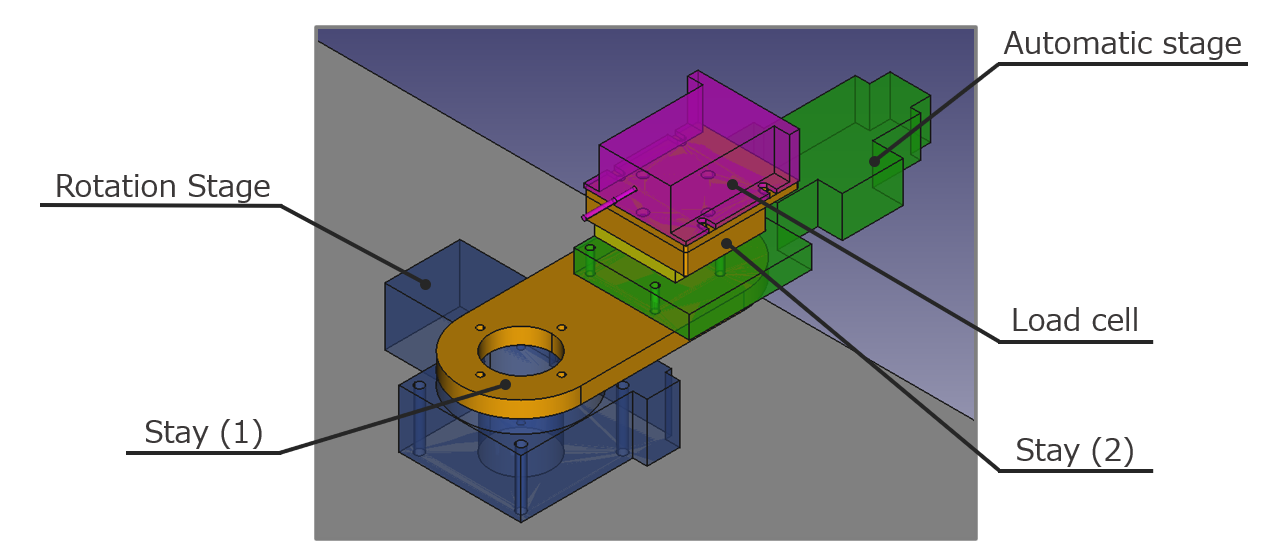
\includegraphics[width=75mm]{images/21-1.png}
        \caption{Acting force measuring device (Photo)} 
    \end{figure_here}
    \begin{figure_here}
        \centering
        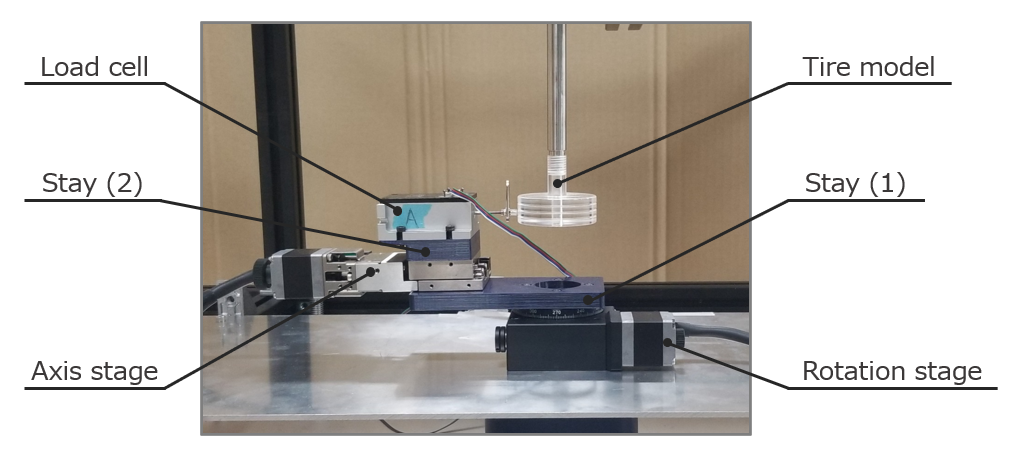
\includegraphics[width=45mm]{images/21-2.png}
        \caption{Mounting part of strain sensors} 
        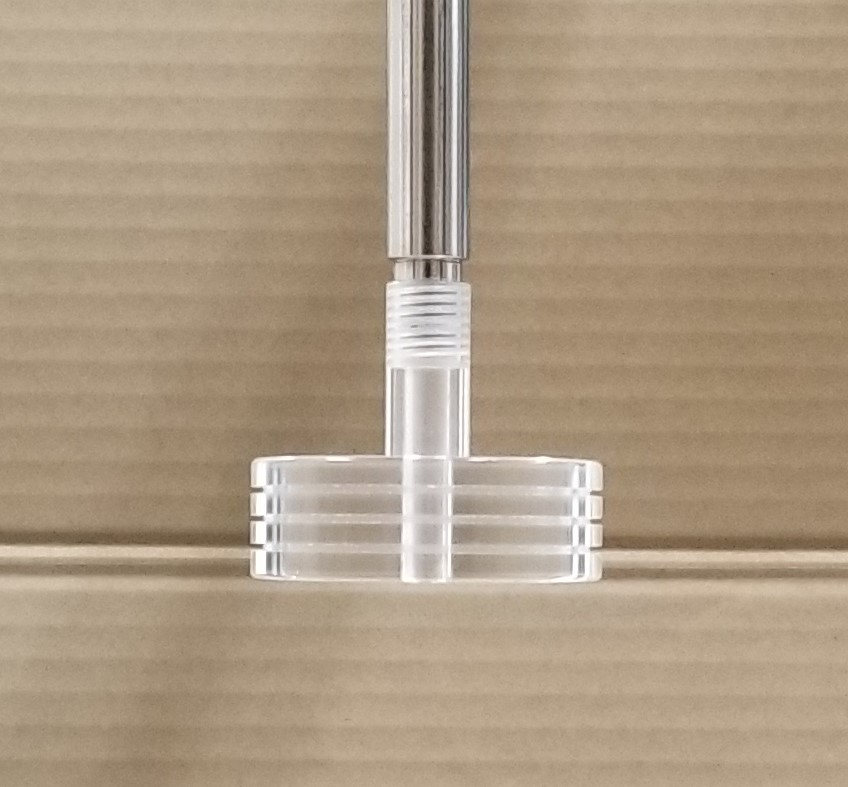
\includegraphics[width=45mm]{images/21-3.png}
        \caption{Mounting part of tire model} 
    \end{figure_here}
\end{multicols}

回流水槽を用いた作用力測定実験の際に使用する作用力測定装置を
性能評価実験を行うため,製作したフレームに組み付けた.
また,本研究において評価対象となるひずみセンサの取付部をFig.に,
作用力を与えるタイヤモデルの取付部をFig.に示している.

\newpage

\subsubsection{測定原理}

Fig.の作用力測定装置のひずみ計測方法には,2ゲージ法を採用している.
また,ひずみセンサはKYOWA製の短軸半導体ひずみセンサ(KSPB-2-120)を使用しており,
一般のひずみセンサのゲージ率が2 $[\Omega]$ 程度であることに比べて
使用した半導体ひずみセンサはゲージ率が 120 $[\Omega]$ 程度と
非常に大きいという特徴がある.これは,回流水槽を用いた作用力測定実験において,
実際に加わる作用力によって生じるひずみを曲げひずみとして測定し,
そのひずみ量は非常に小さいことから,これを測定するためにゲージ率の大きい
高感度の半導体ひずみセンサを使用し,2ゲージ法によってひずみセンサ単体の場合に比べて,
2倍の出力電圧を得ることができるためである.
したがって,作用力測定装置に加わる微小なひずみを測定することを目的としており,
作用力測定実験に適した測定方法であるといえる.

\subsection{校正実験装置}
本研究において製作・使用した実験装置の概略図および写真を以下のFig.,Fig.に示す.

\begin{figure}[htbp]
    \footnotesize
    \begin{center}
        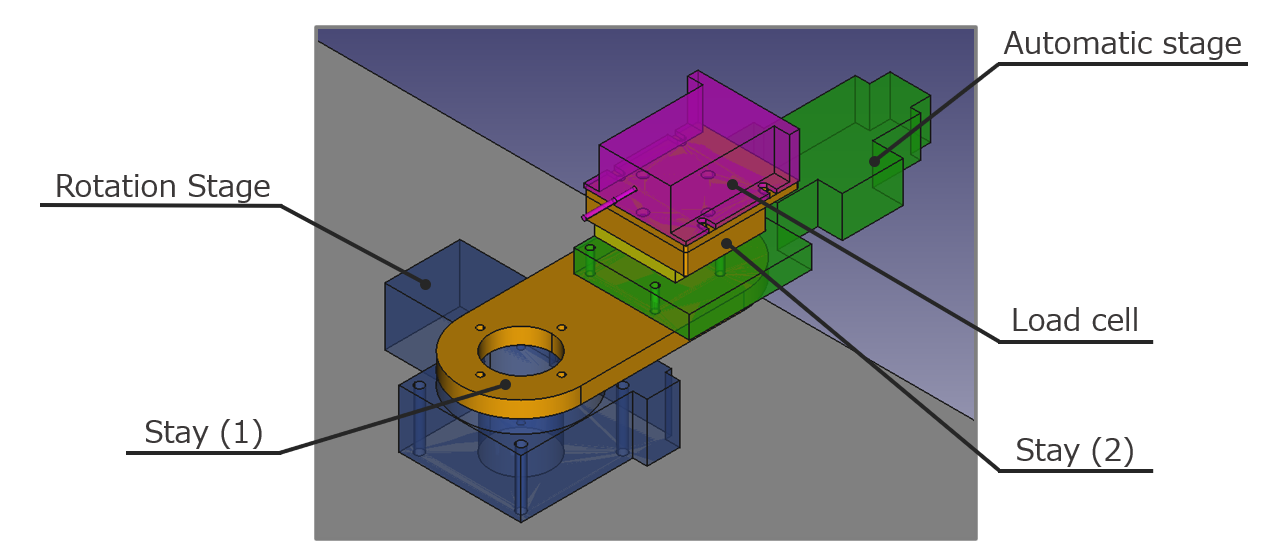
\includegraphics[width=120mm]{images/22-1.png}
        \caption{Calibration device (3D CAD)}
        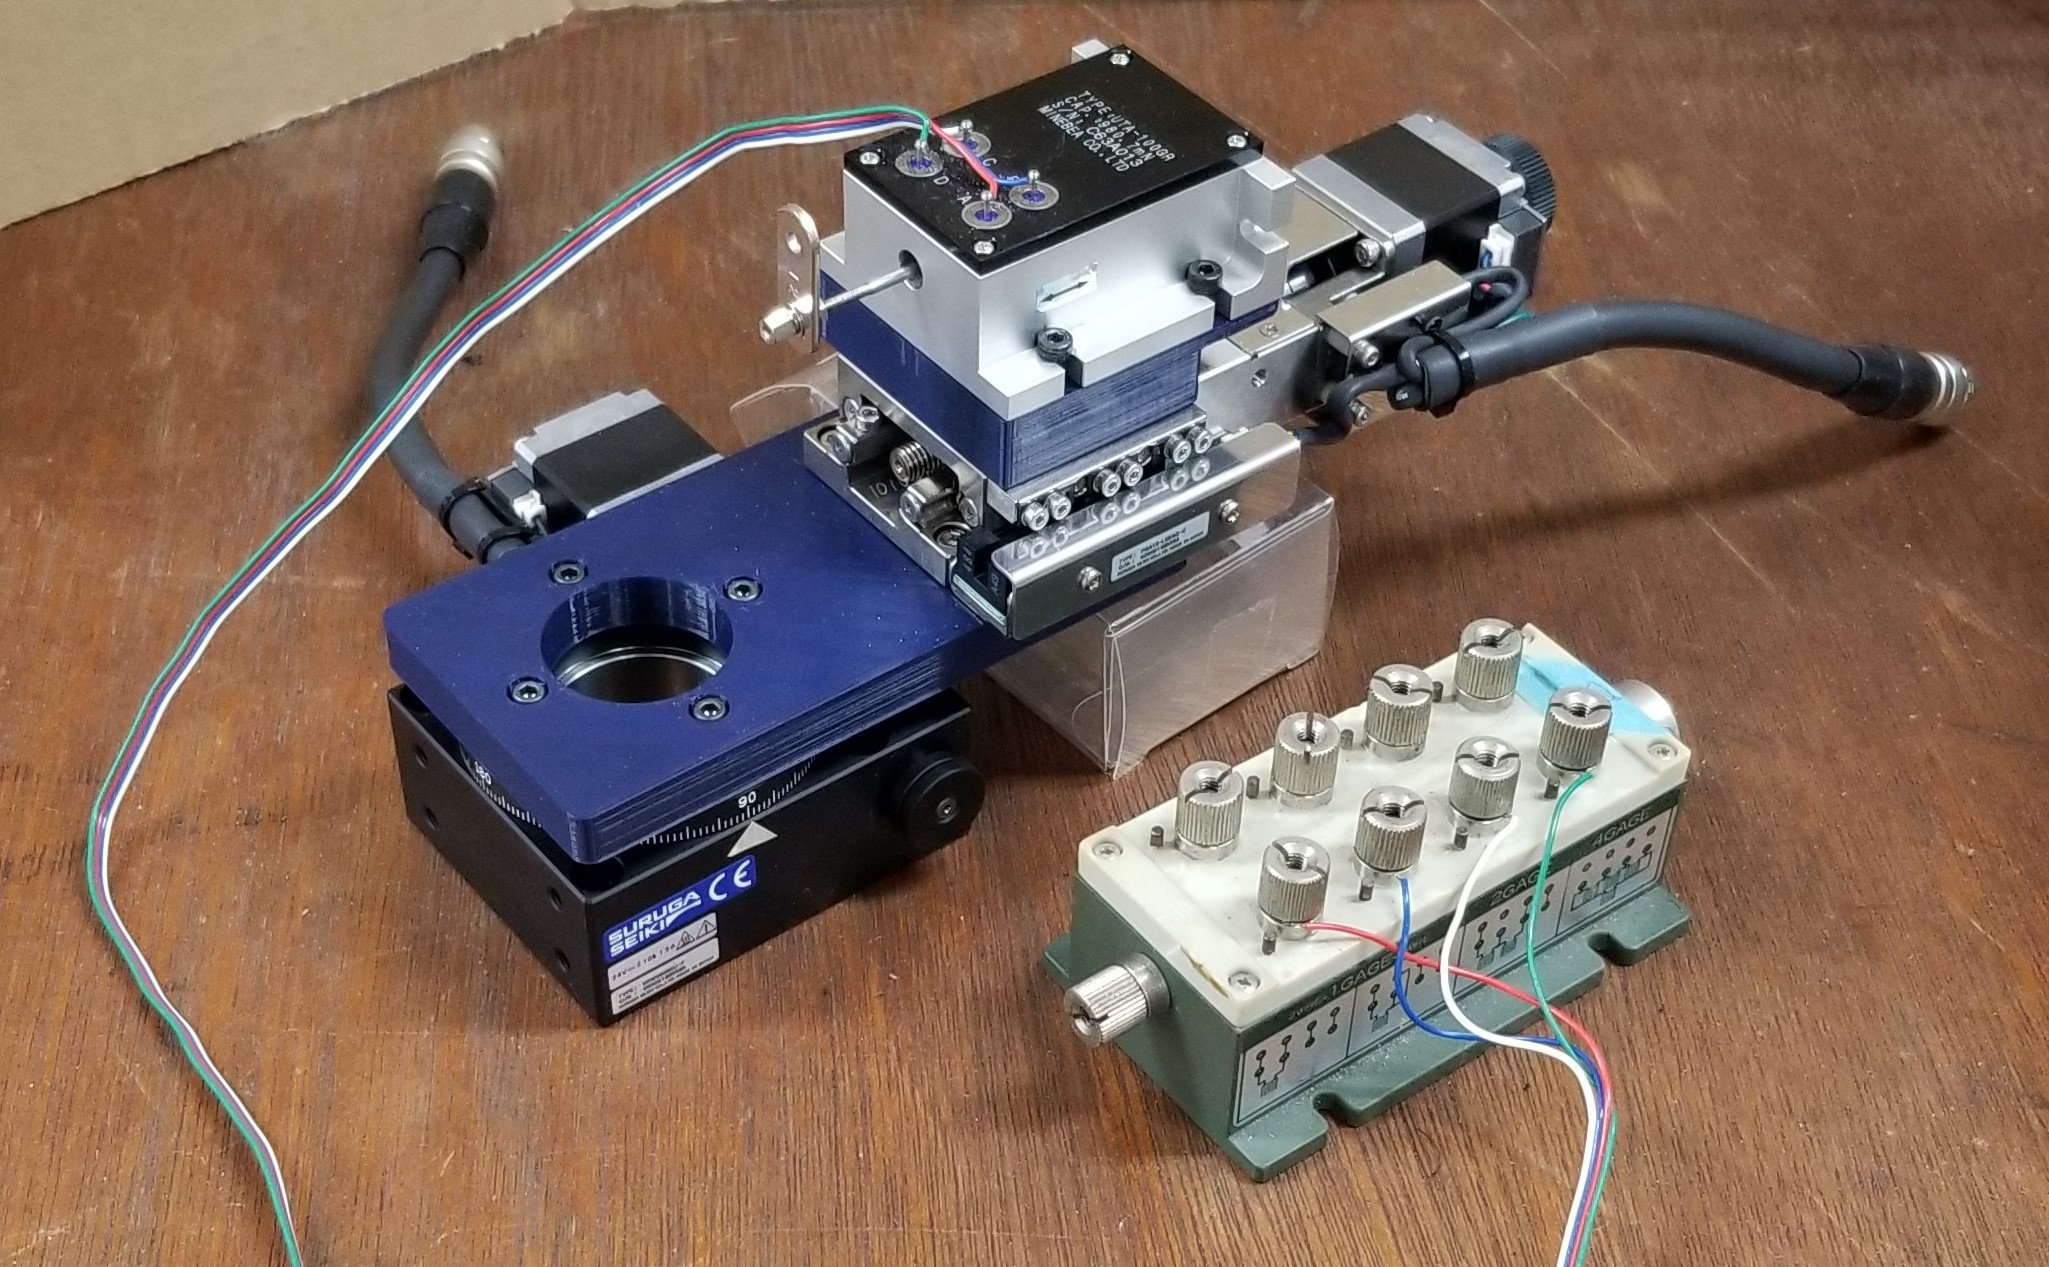
\includegraphics[width=80mm]{images/22-2.png}
        \caption{Calibration device (Photo)}
    \end{center}
\end{figure}

\newpage

校正装置は,作用力測定装置に取り付けられた2組のひずみセンサについて,
作用力の角度による出力電圧の関係性を調べる目的がある.
また,自動ステージを用いて人為的な操作を可能な限り減らし自動化することで,
不本意なノイズの削減や複数回の実験を効率的に行うことができた.
作用力を与える校正装置(Fig.)は,自動一軸ステージ,自動回転ステージ,ロードセル,
それらを接続するステーから構成される.

また,作用力測定装置のフレームに校正実験装置を取り付けることで,
作用力測定と校正実験装置の位置関係を保持することができる.(Fig.)
校正実験装置はアルミ板を介してフレームに取り付ける.
設置の際には,作用力測定装置をフレーム上に設置し,
作用力測定装置の回転軸と自動回転ステージの回転軸を
できるだけ一致させるように調整をしながら行うことが好ましい.
\begin{figure}[htbp]
    \footnotesize
    \begin{center}
        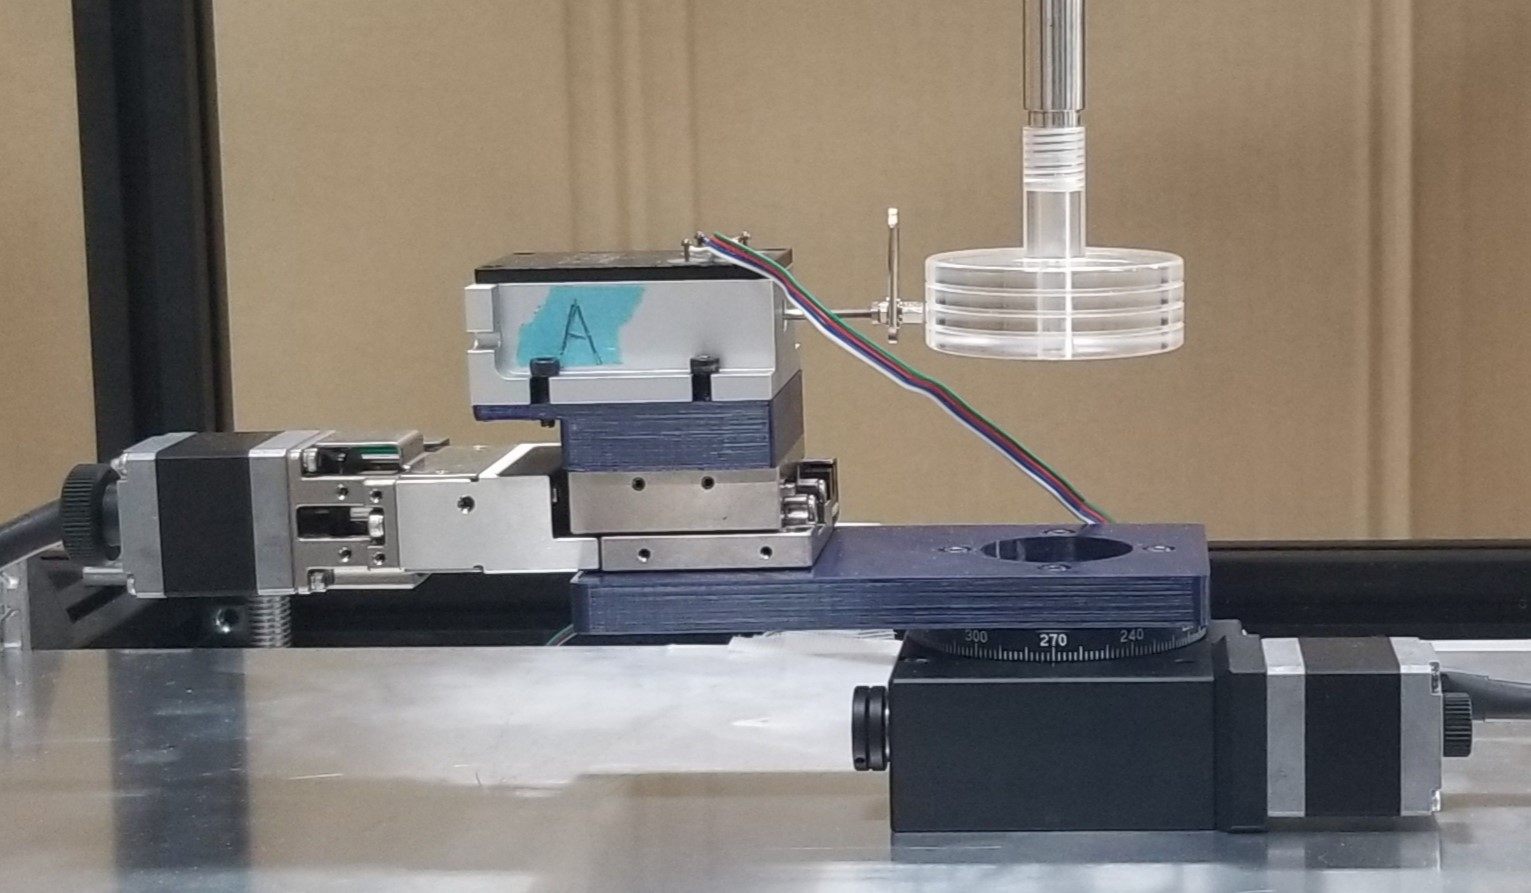
\includegraphics[width=80mm]{images/22-3.png}
        \caption{Assembled calibaration device}
    \end{center}
\end{figure}

なお,本研究では,ロードセルはミネベアミツミ製 微小荷重引張圧縮型 UTA (UTA-100GR),
自動一軸ステージは駿河精機製 リニアボールガイドステージ (PG530),
自動回転ステージは駿河精機製 回転ステージ ウォームギア (KRW06360),
自動ステージコントローラは駿河精機製 ステッピングモータコントローラ(DS102MS) を使用している.
また,2つのステーについては,自動回転ステージ上に取り付けることになり,
軽量である必要があるため3Dプリンタを用いて製作し,使用している.
% ジョイントの形状や材料の充填率を
% 変更しながら重量と剛性のバランスを調整しながら製作を行った.

\begin{figure}[htbp]
    \footnotesize
    \begin{center}
        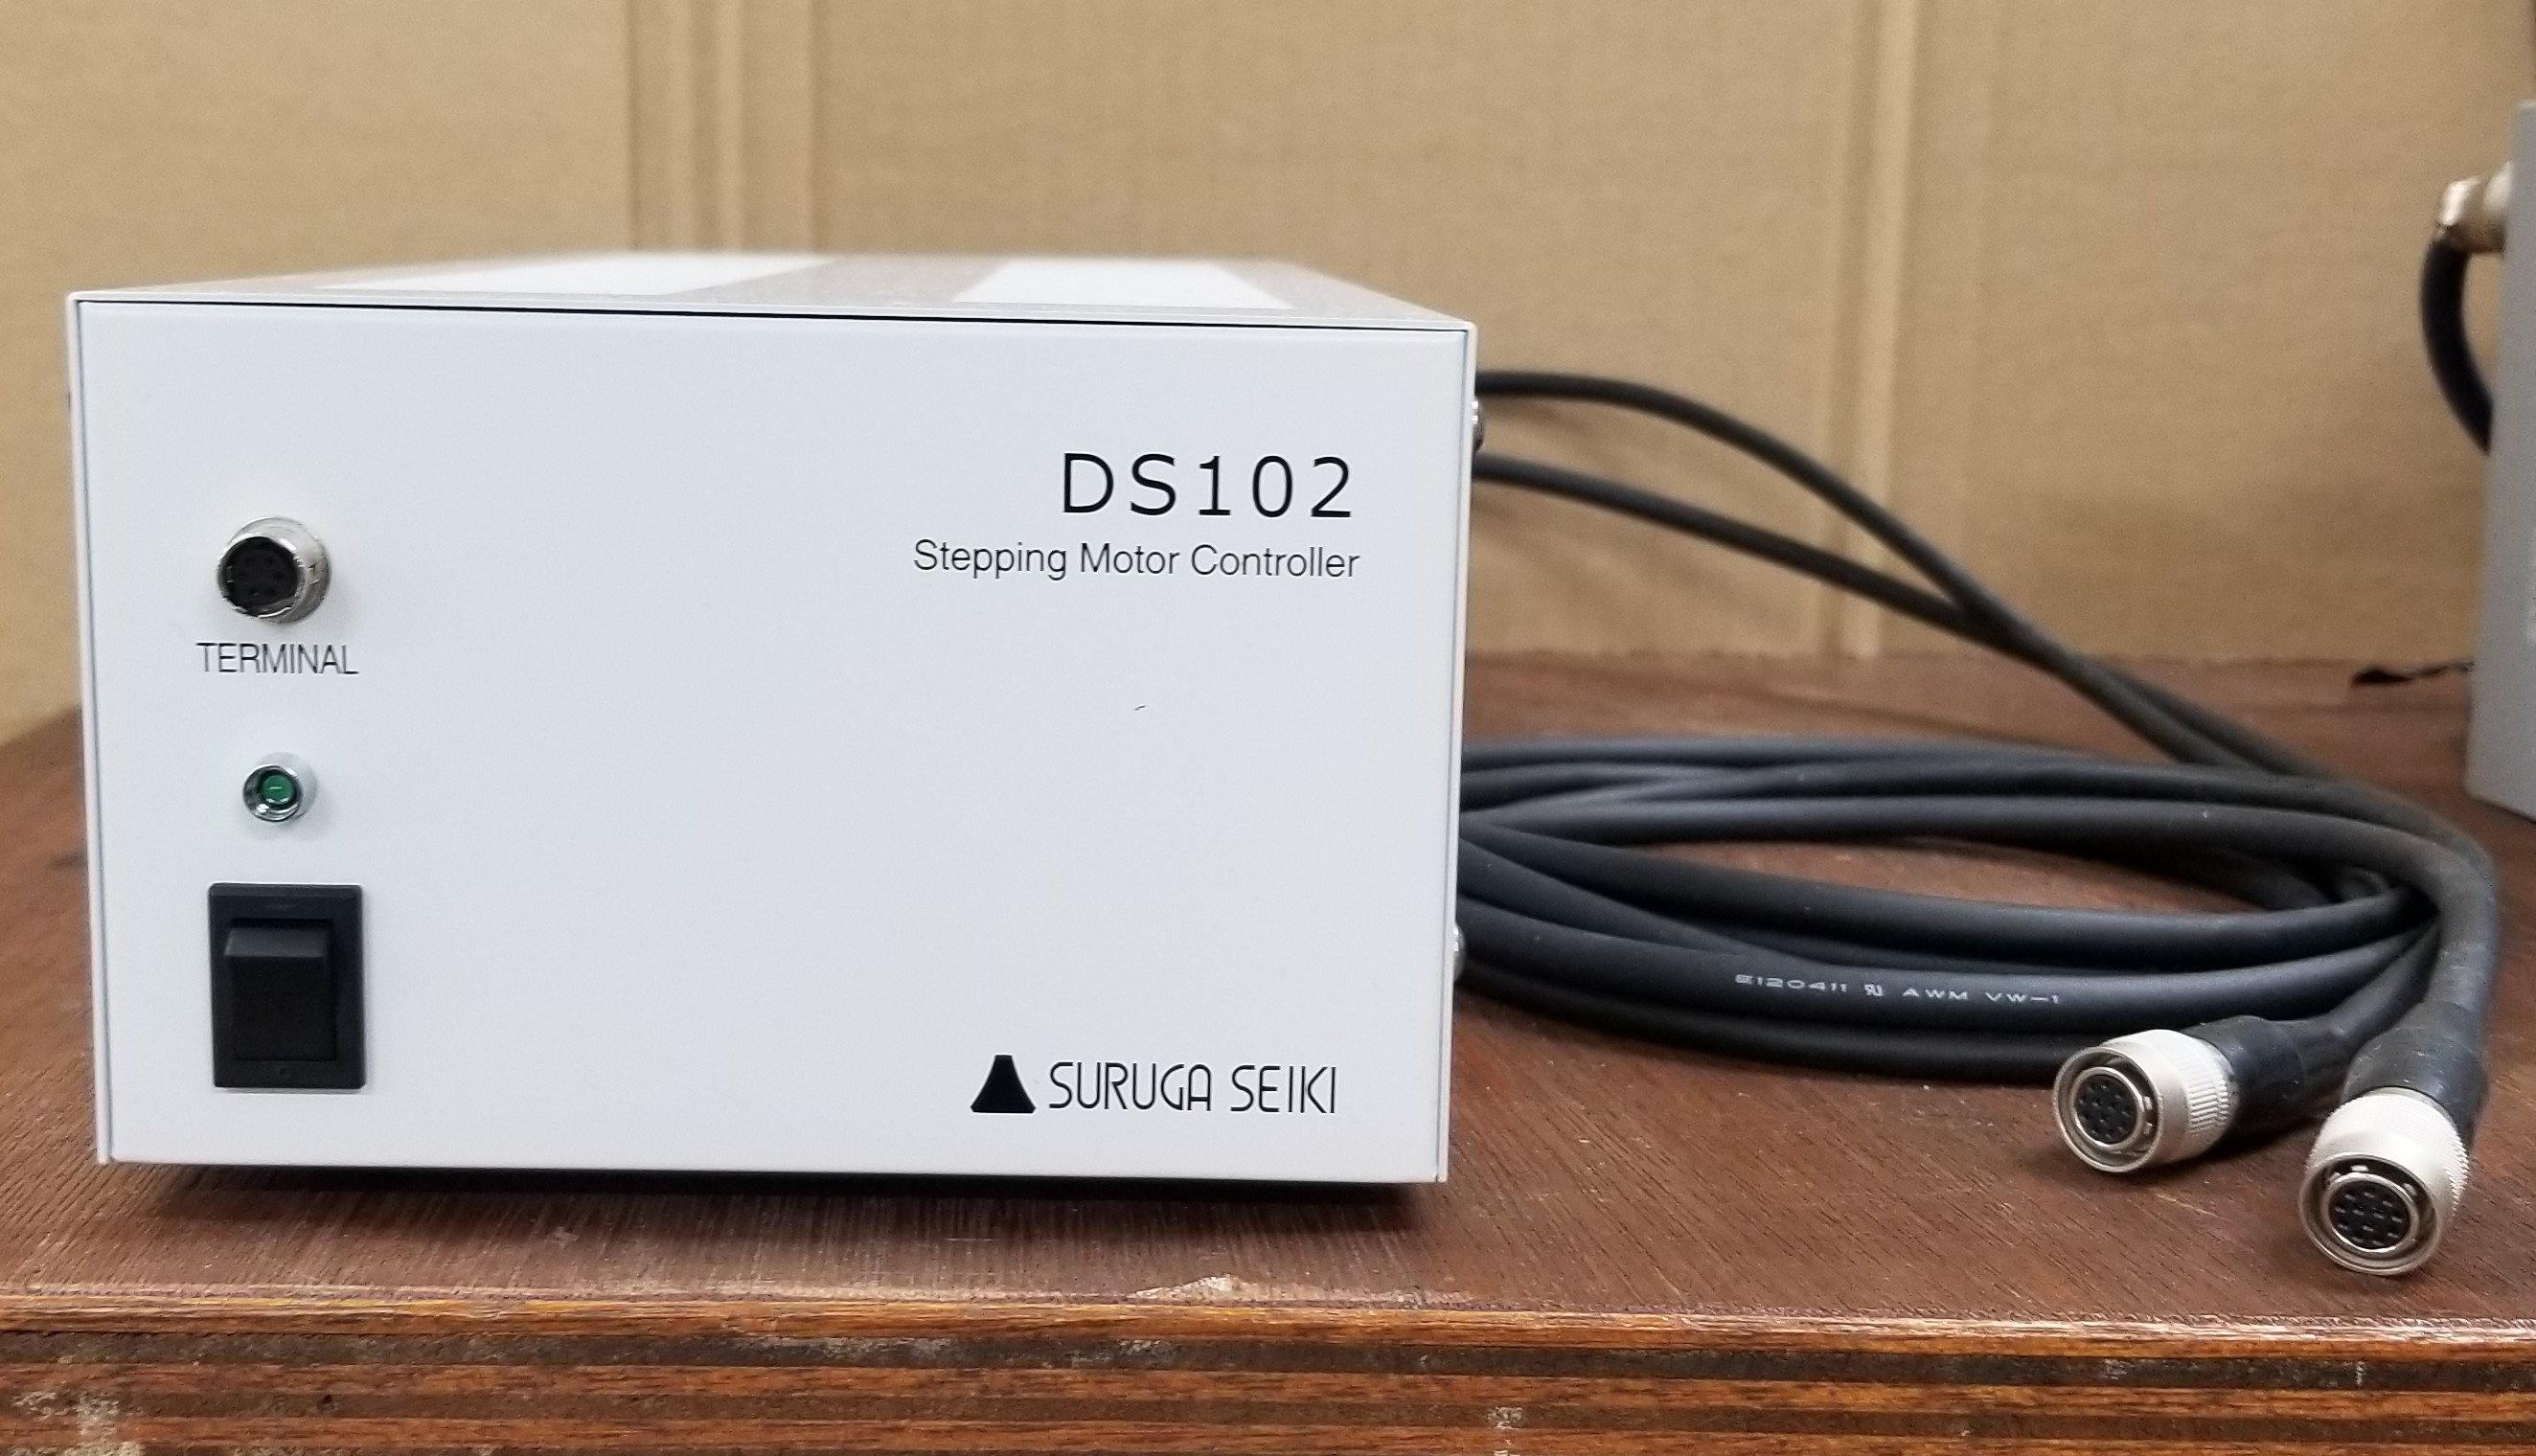
\includegraphics[width=80mm]{images/22-4.png}
        \caption{Stage Controller}
    \end{center}
\end{figure}

\newpage

また,作用力測定装置のひずみセンサ,校正実験装置に取り付けられたロードセルからの出力電圧は
Fig.に示すロードセルおよびひずみセンサに対応したそれぞれのストレインアンプを通して,
データロガーへと送られ,データロガーに接続されたPCへと保存される.
ロードセルの接続されるストレインアンプ(灰,2個)は,ミネベアミツミ製 動ひずみ測定器(DSA-631),
ひずみセンサの接続されるストレイアンプ(黒,1個)は,ミネベアミツミ製 動ひずみ測定器(DSA-605C),
データロガーには,GRAPHTEC製 高電圧高速 4チャンネルロガー(GL2000) を使用している.

\begin{figure}[htbp]
    \footnotesize
    \begin{center}
        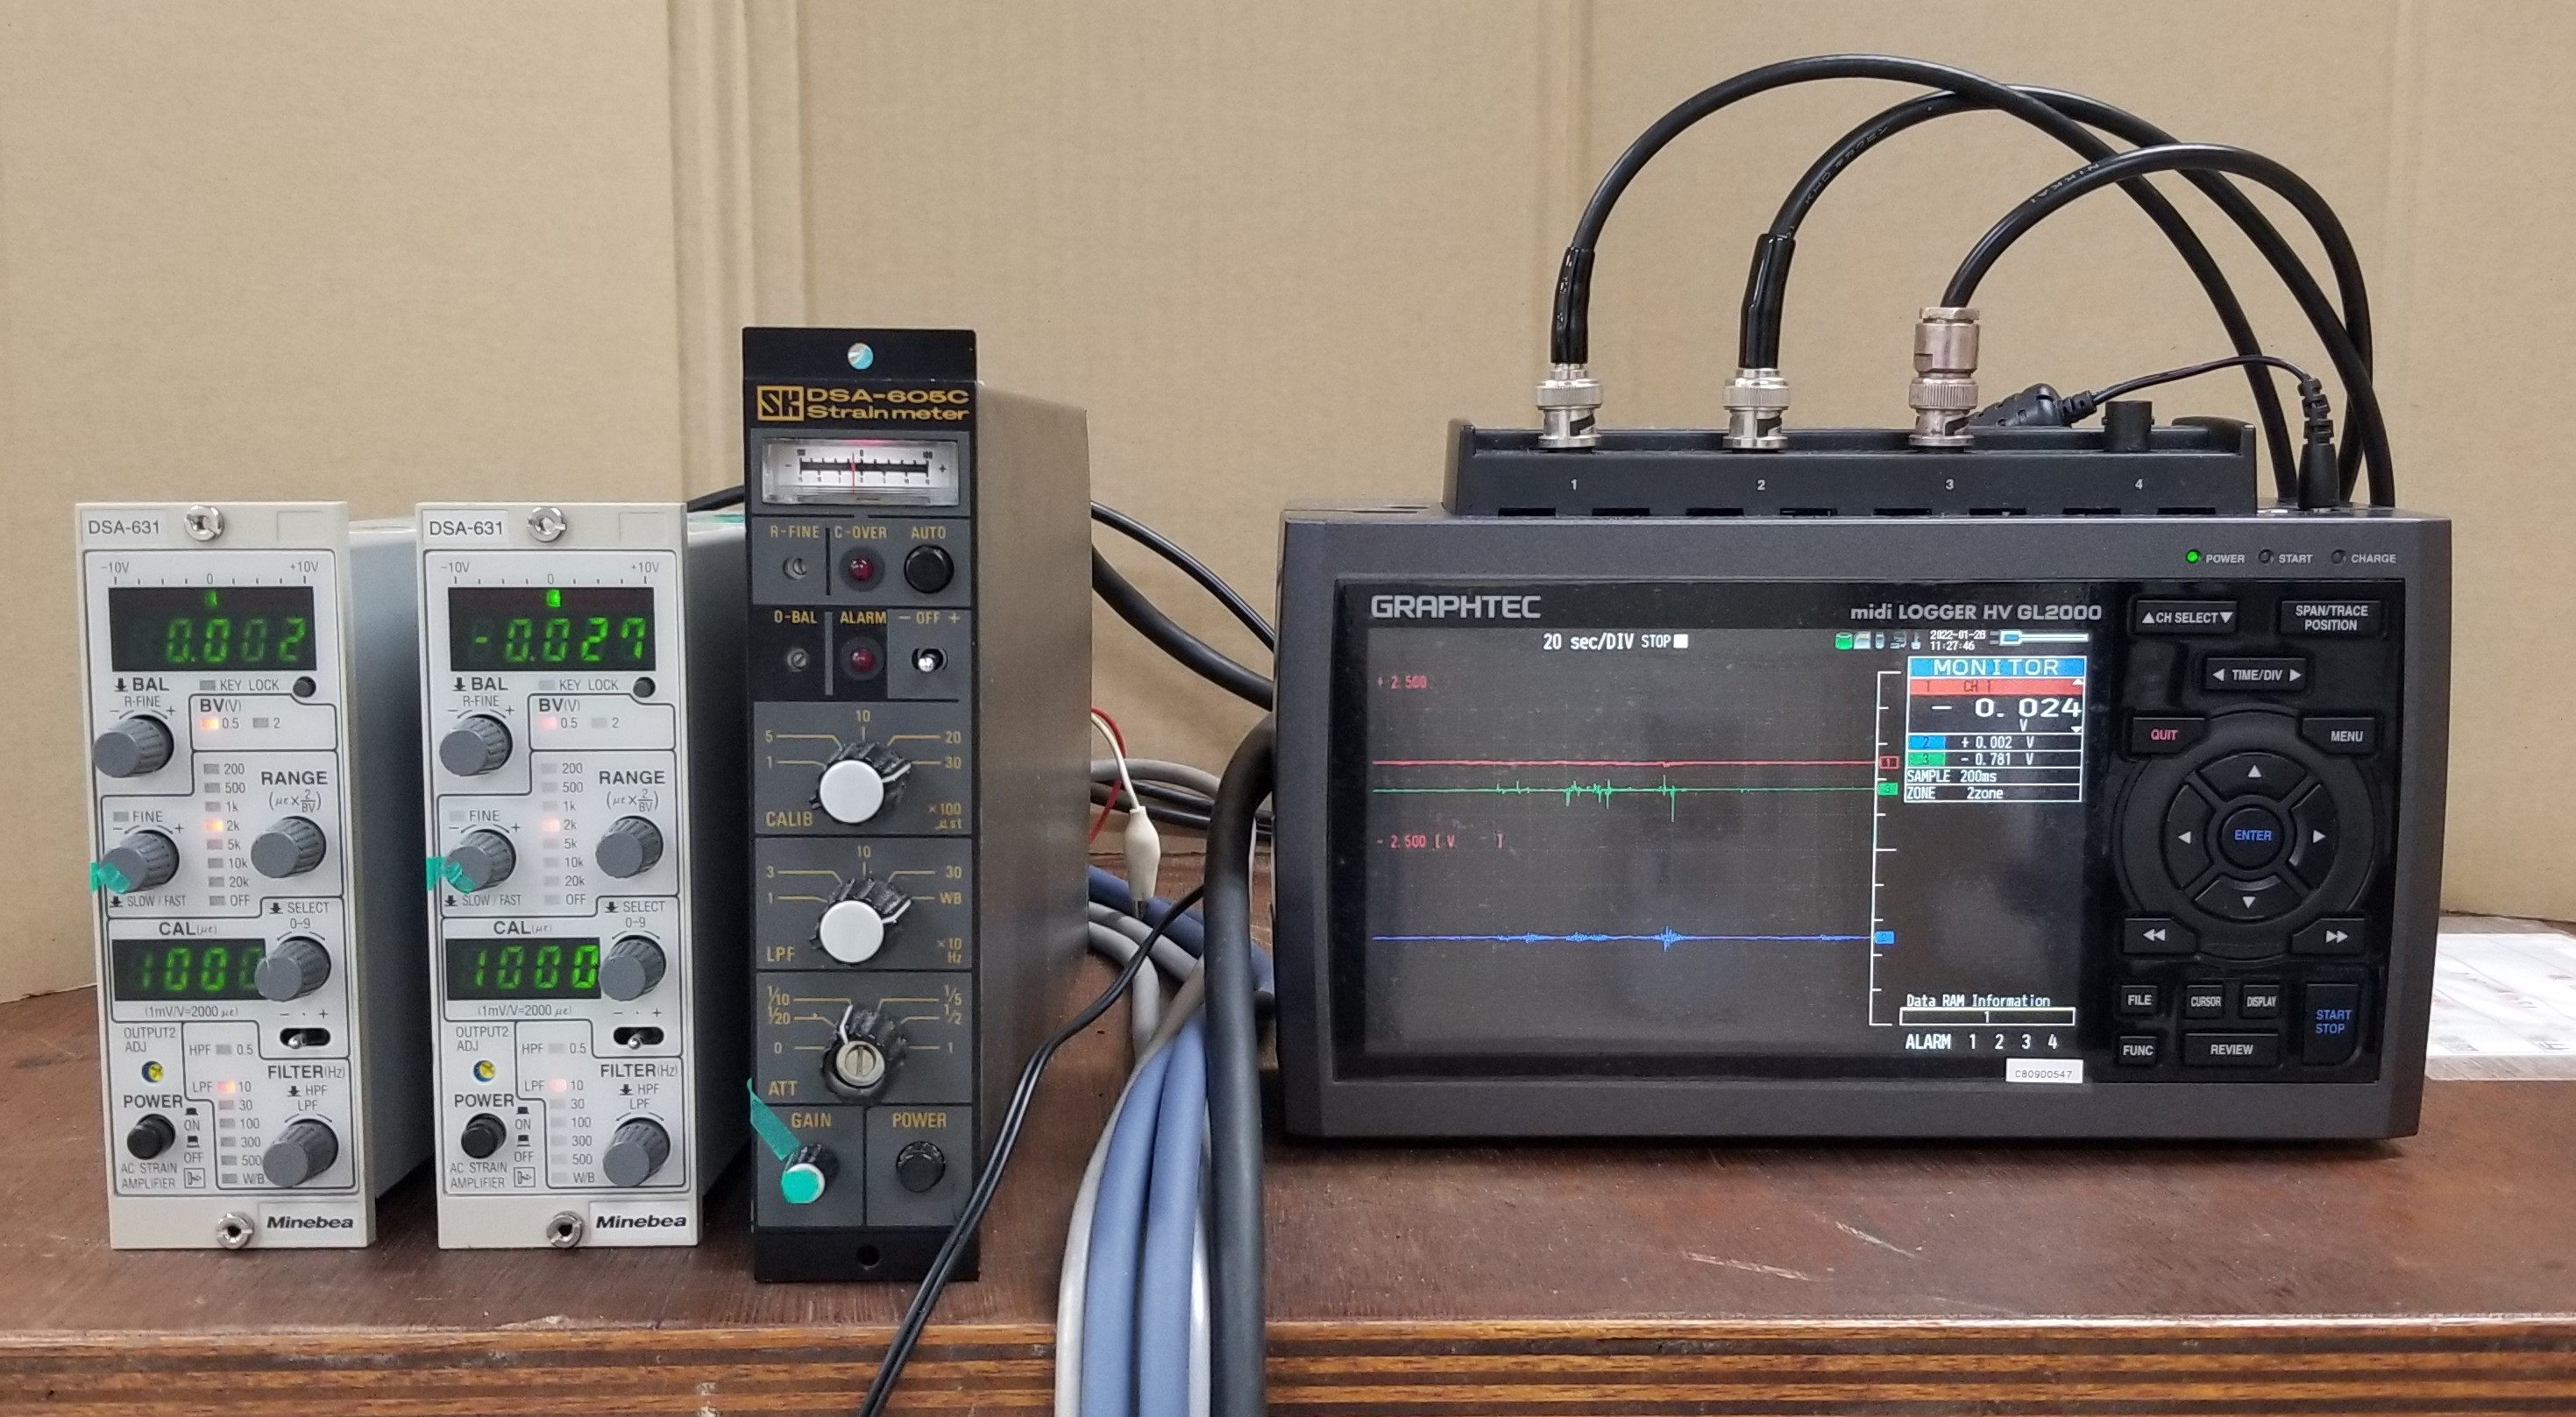
\includegraphics[width=85mm]{images/22-5.png}
        \caption{Strain Amplilifiers and data logger}
    \end{center}
\end{figure}

以下のFig.に本研究で使用した実験装置について,概略図を示す.

\begin{figure}[htbp]
    \footnotesize
    \begin{center}
        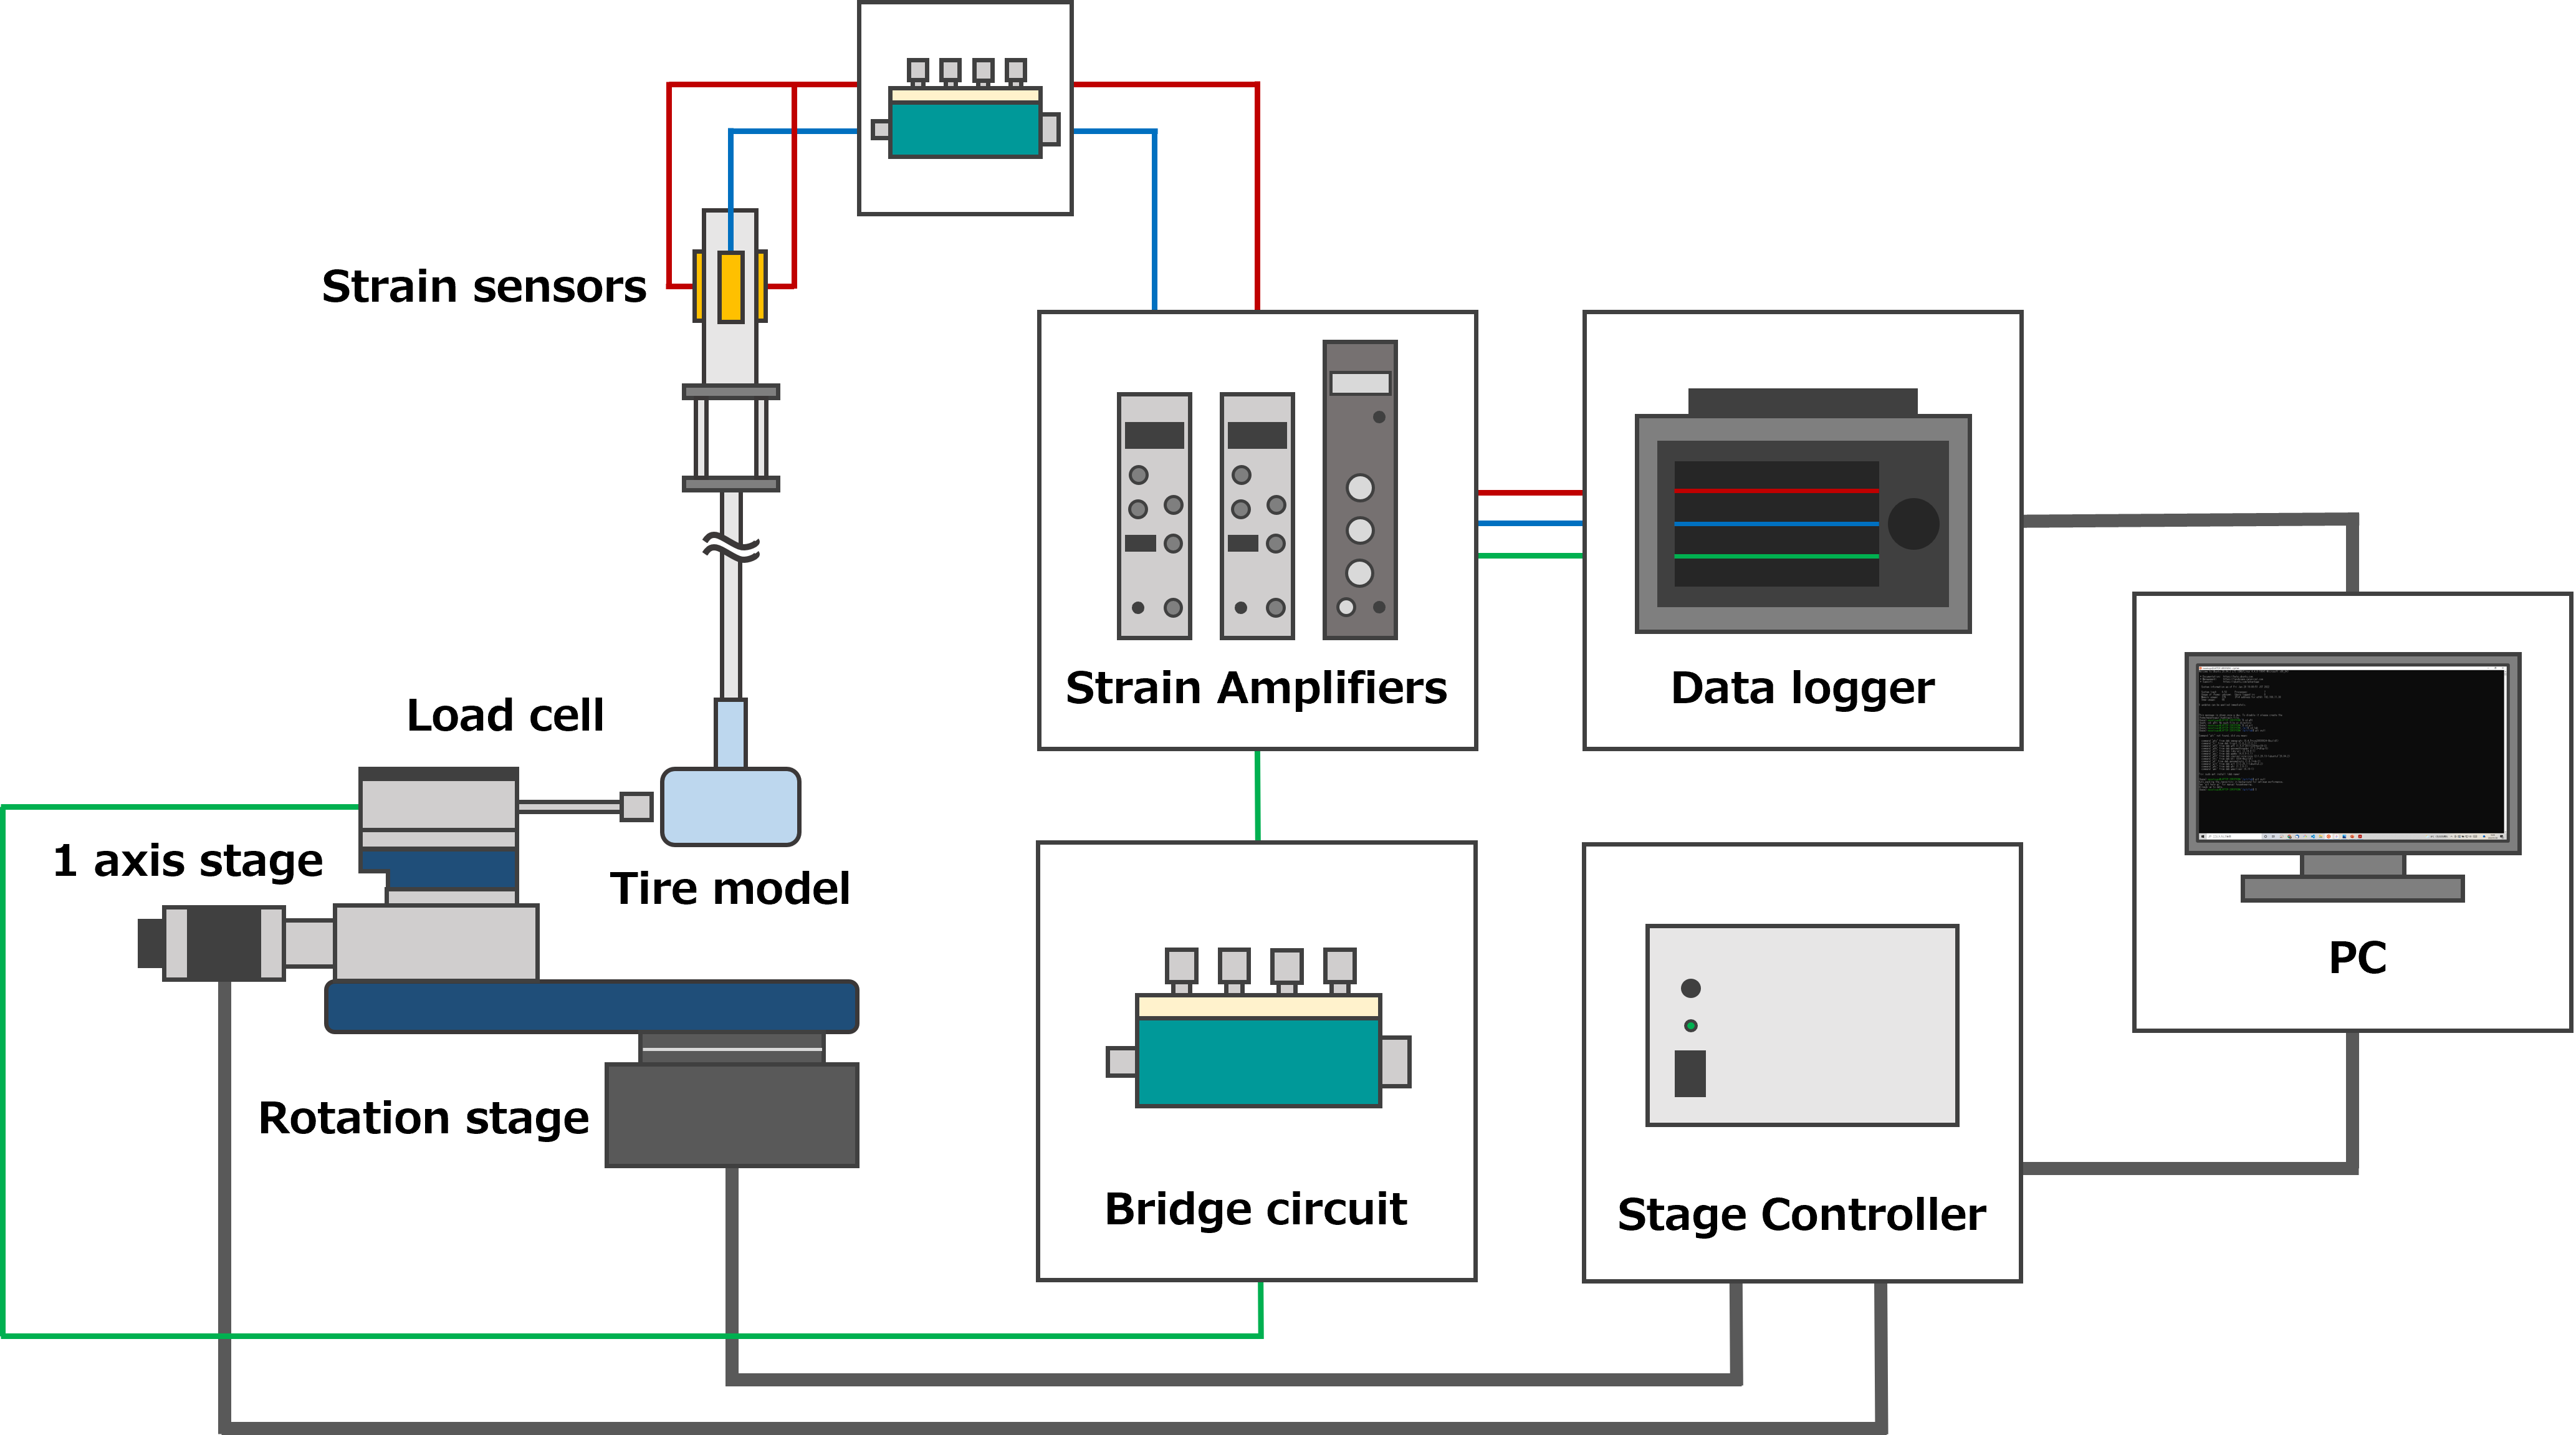
\includegraphics[width=140mm]{images/22-6.png}
        \caption{Schematic of experimental system}
    \end{center}
\end{figure}
\newpage
\section{校正理論}
作用力測定装置から得た抗力方向および揚力方向における出力電圧$V_D$,$V_L$を
正規座標系の$x$軸方向および$y$軸方向の荷重$F_x$,$F_y$に換算する際に,
出力電圧$V_D$,$V_L$と$F_x$,$F_y$の関係性を明らかにするための校正実験を
行う必要がある.
校正実験によって得られた結果を用いて関係性を明らかにするための校正理論について述べる.

\subsection{作用力測定装置と校正実験装置の関係}
はじめに,作用力測定装置と校正実験装置の関係について説明する.

作用力測定装置と校正実験装置の設置位置によって校正実験結果は大きく変動するため,
その影響を考慮し,補正処理を行う必要がある.
このとき以下のような要因が,校正実験結果への影響を与えていると考えられる.

\begin{enumerate}[(1)]
    \item 作用力測定装置にひずみセンサが正確に取り付けることが難しい
    \item 作用力測定装置が回流水槽に正確に設置することが難しい
    \item 作用力測定装置と校正装置の回転軸を一致させることが難しい
\end{enumerate}

ここで,水流に対する座標系を正規座標系 $(x,y)$,
作用力測定装置の座標系を座標系(1) $(x',y')$,
校正装置の座標系を座標系(2) $(x,'' y'')$とする.

このとき,(1) 作用力測定装置にひずみセンサを正確に取り付けることが難しいこと,
(2) 作用力測定装置が回流水槽に正確に設置することが難しいことから,
座標系[1]は正規座標系に対して
$x'$軸は$x$軸から$\theta_x$,$y'$軸は$y$軸から$\theta_y$だけ回転している.
また,座標系[2]は正規座標系に対して
$x''$軸は$x$軸から$y$方向に$\Delta x$,
$y''$軸は$y$軸から$x$方向に$\Delta y$だけオフセットを持つ状態となる.

\begin{figure}[htbp]
    \footnotesize
    \begin{center}
        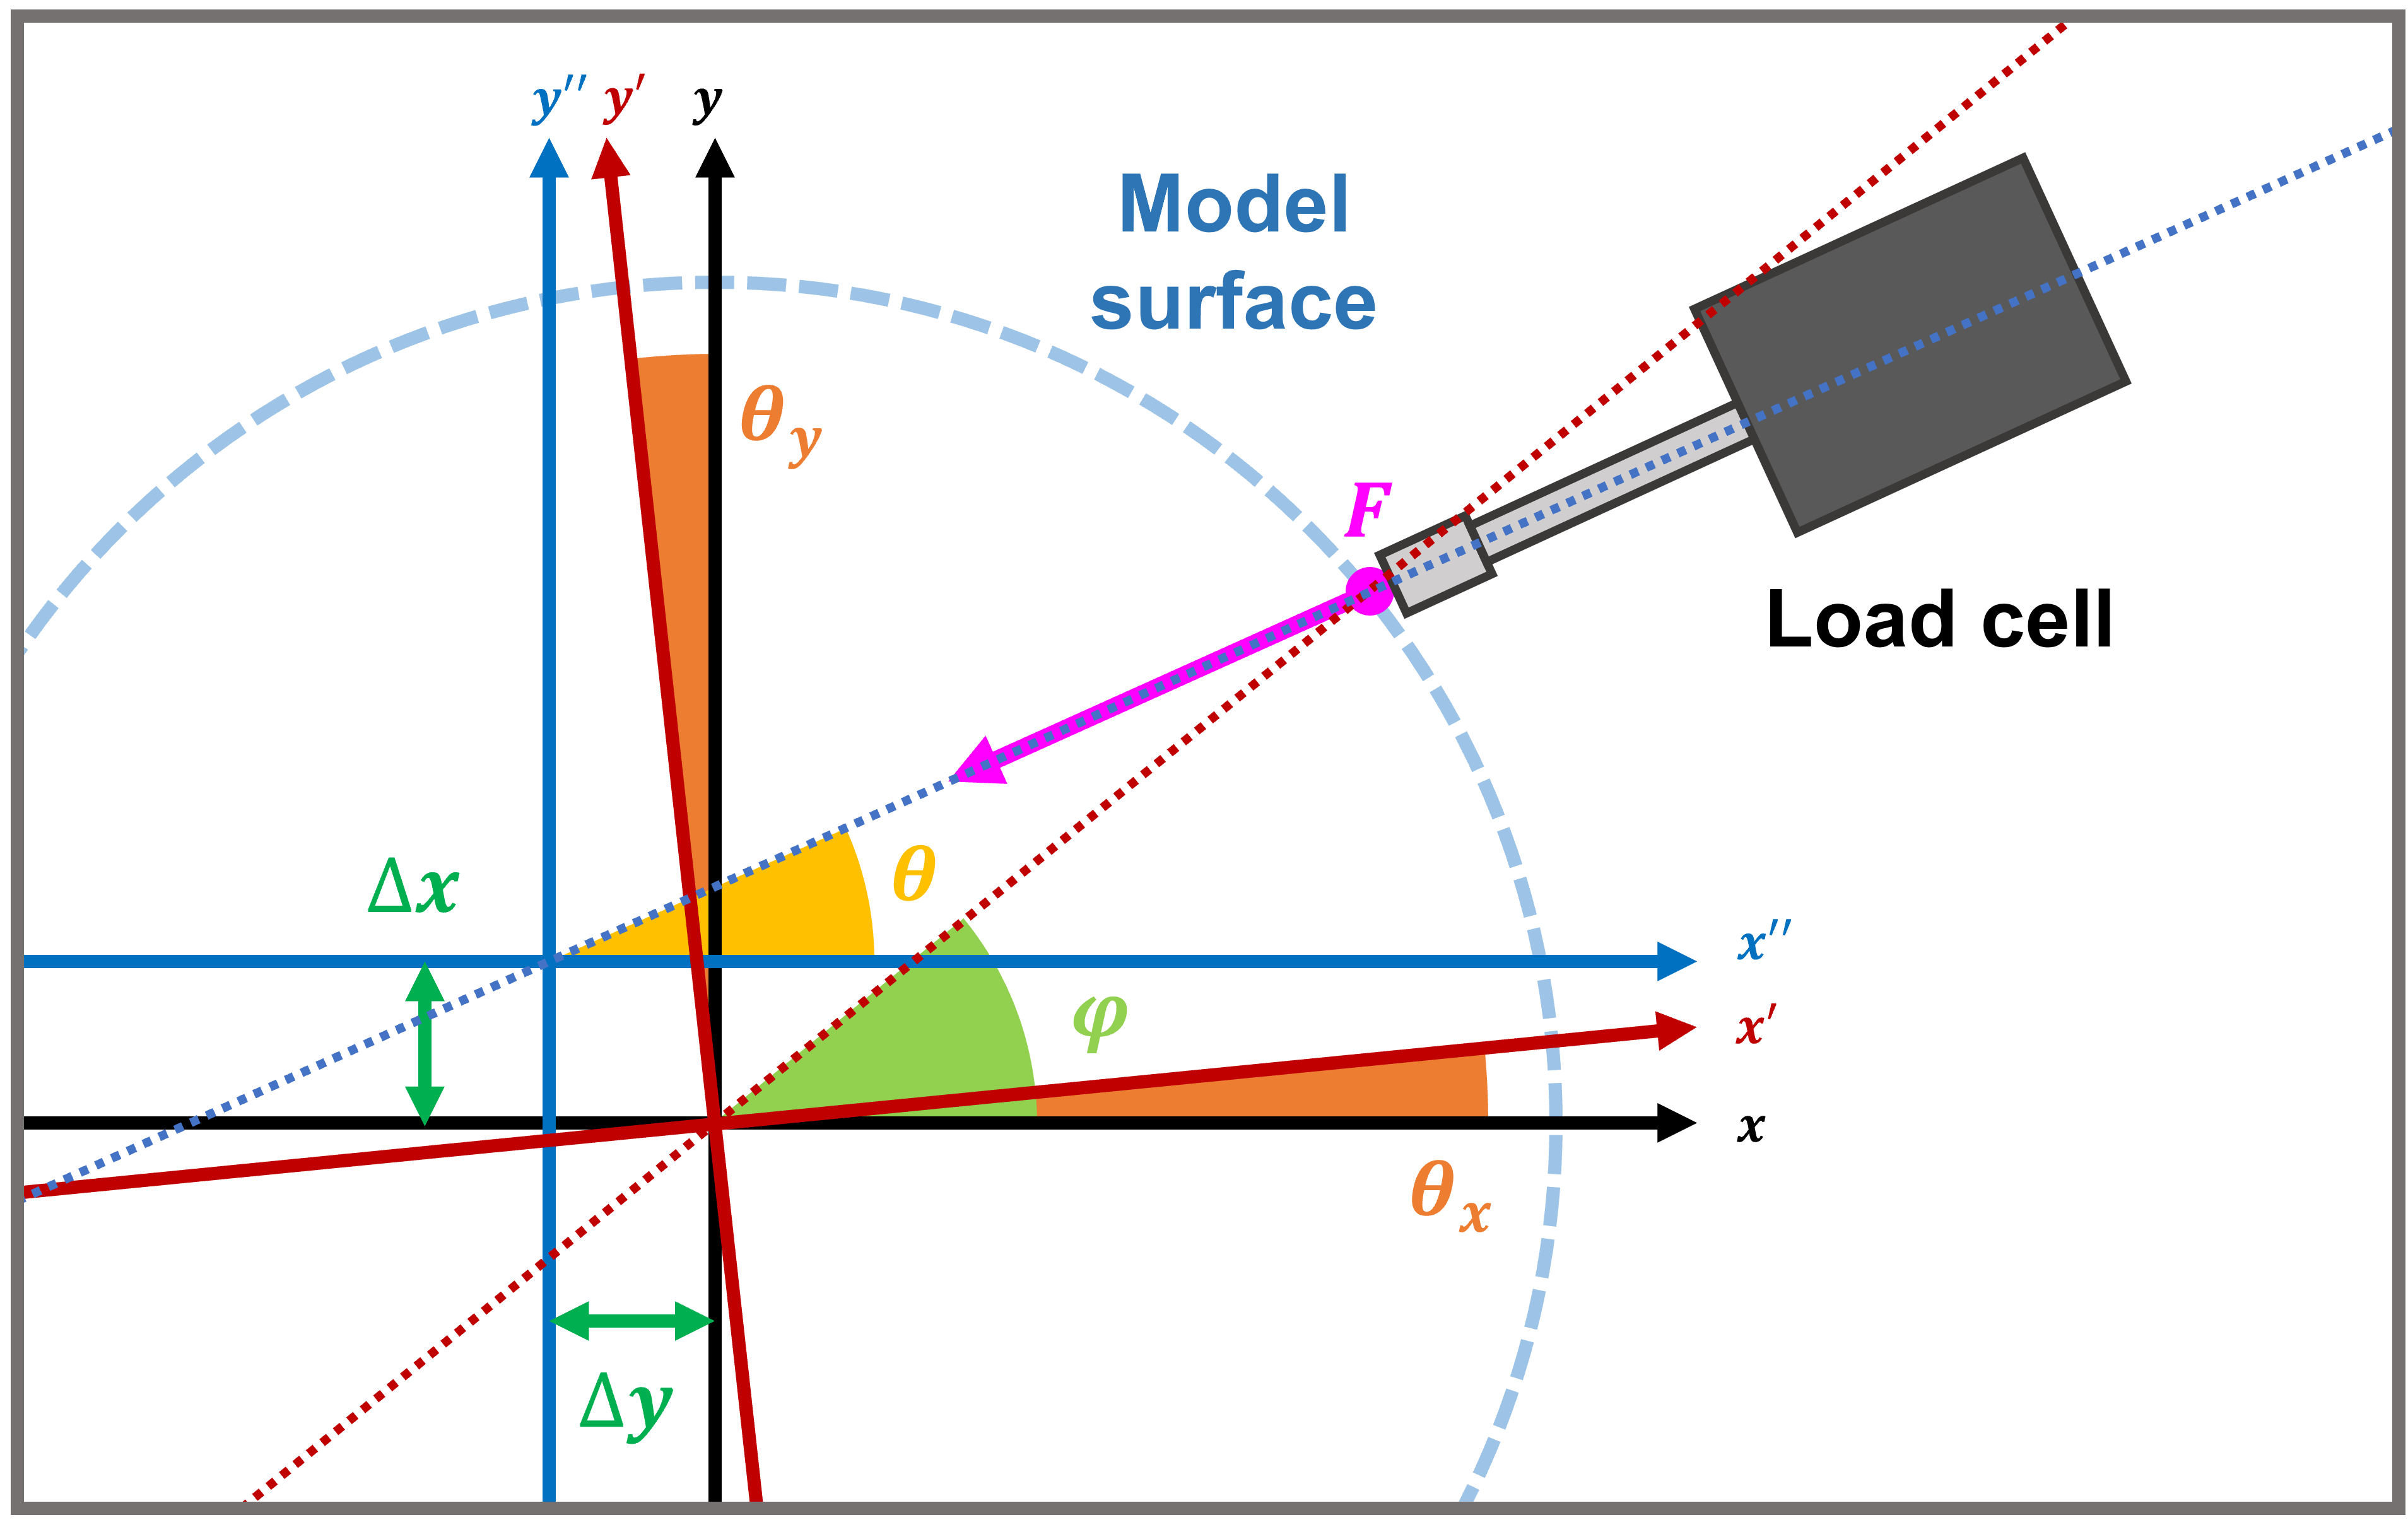
\includegraphics[width=80mm]{images/31-1.png}
        \caption{}
    \end{center}
\end{figure}

\newpage

\subsection{出力電圧勾配}

作用力測定装置の評価にあたり,作用力測定装置に取り付けられた2組のひずみセンサ
および校正実験の際に作用力を与えるロードセルの出力電圧の対応関係を調べることで評価を行う.
ここで,作用力測定装置において抗力方向のひずみセンサの出力電圧を$V_d$,揚力方向を$V_l$,
ロードセルの出力電圧を$V$とするとき,抗力方向の出力電圧勾配を$v_d$,
揚力方向の出力電圧勾配を$v_l$として以下のように表す.

\begin{align}
    v_d = V_d / V \\
    v_l = V_l / V
\end{align}

\subsection{座標系の回転における補正理論}

正規座標系と座標系[1]の回転における補正理論を説明する.
ここでは,座標系のオフセットはない($\Delta x = 0$,$\Delta y = 0$)として考える.
上述の通り正規座標系と座標系[1]について,以下のFig.のように回転角$\theta_{x}$,$\theta_{y}$を持つ.
ここで,作用力$F$を与えるとそれぞれの方向に作用力$F_{x}$,$F_{y}$,$F_{x'}$,$F_{y'}$が加わる.
このとき,作用力測定装置から得られる電圧$V_{x'}$,$V_{y'}$は作用力$F_{x'}$,$F_{y'}$に起因するものである.
また,得られた出力電圧$V_{x'}$,$V_{y'}$から,ロードセルの出力電圧$V_1$を用いて
出力電圧勾配$v_{x'}$,$v_{y'}$を求めることができる.
したがって,正規座標系と座標系[1]の関係について,
$v_{x}$と$v_{x'}$および$v_{y}$と$v_{y'}$の関係を明らかにすれば良い,

\begin{figure}[htbp]
    \footnotesize
    \begin{center}
        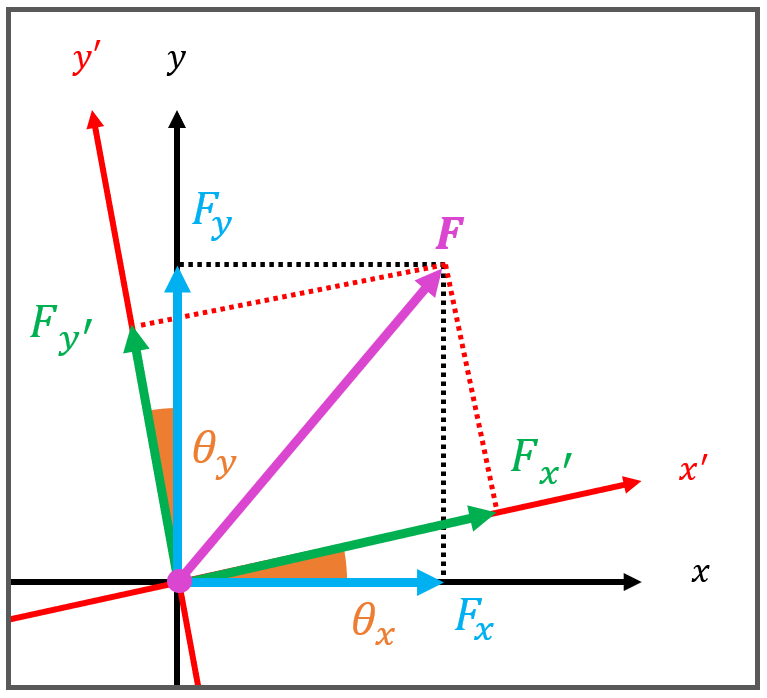
\includegraphics[width=75mm]{images/33-1.png}
        \caption{}
    \end{center}
\end{figure}

\subsubsection{回転角$\theta_{x}$,$\theta_{y}$の算出}
はじめに,回転角$\theta_{x}$,$\theta_{y}$を算出する.
理論式における$v_{x\;\mathrm{theory}}$及び$v_{y\;\mathrm{theory}}$は正弦波とその位相差で表すことができる.
したがって,校正実験結果の各角度の出力電圧勾配においても同様の正弦波と
その位相差で表すことが可能であると予想することができる.
このとき,離散フーリエ変換を適用し,
波数1の成分について,実部を$Re$,虚部を$Im$として
位相角$\phi$を求めることができる.

\begin{align}
    \phi = \arctan \left(\frac{Im}{Re}\right) \cdot \frac{180}{\pi}
\end{align}
\vskip \baselineskip

抗力方向の結果から得られた位相角を$\phi_1$,揚力方向から得られた位相角を$\phi_2$と
するとき,抗力方向の出力電圧勾配$v_d$と
正規座標系における$x$軸方向の出力電圧勾配の理論値$v_{x\;\mathrm{theory}}$との位相差
$\theta_x$,
揚力方向の出力電圧勾配$v_l$と
正規座標系における$y$軸方向の出力電圧勾配の理論値$v_{y\;\mathrm{theory}}$との位相差
$\theta_y$を以下のように表される.

\begin{align}
    \theta_x = \pi - \phi_1 \\
    \theta_y = \frac{\pi}{2} - \phi_2
\end{align}
\vskip \baselineskip

したがって,$x'$軸,$y'$軸は左回りを正方向として,それぞれ$\theta_x$,$\theta_y$だけ
回転していることとなる.
また,作用力測定装置に取り付けられた抗力・揚力方向のひずみセンサの取付角$\phi_s$は
位相角$\phi_1$,$\phi_2$より求めることができる.

\begin{align}
    \phi_s = \left| \phi_1 - \phi_2 \right|
\end{align}

\newpage

\subsubsection{出力電圧勾配の座標変換}

位相角$\theta_x$,$\theta_y$が求められたことから,
それらを用いて出力電圧勾配の座標変換を行う.
ここで,座標系[1]の$x'$軸,$y'$軸を
それぞれ$f_{x}\left(x\right)$,$f_{y}\left(x\right)$として,
正規座標軸の$x$を用いた式で表す.

\begin{figure}[htbp]
    \footnotesize
    \begin{center}
        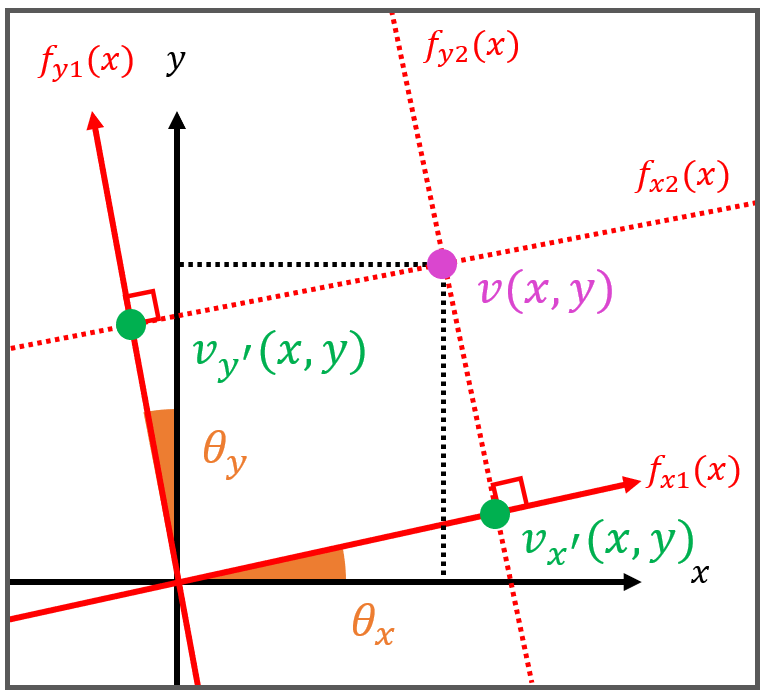
\includegraphics[width=75mm]{images/33-2.png}
        \caption{}
    \end{center}
\end{figure}

算出した位相角$\theta_x$,$\theta_y$より,$f_{x}\left(x\right)$,$f_{y}\left(x\right)$は
以下のように表される.

\begin{align}
    f_{x}\left(x\right) & = \tan \theta_x \; x            \\
    f_{y}\left(x\right) & = - \frac{1}{\tan \theta_y}\; x
\end{align}
\vskip \baselineskip

このとき,作用力$F$は,Fig.に示す点$F$の座標を表すベクトルと考えることができる.
また,その座標はFig.より,$f_{x}\left(x\right)$,$f_{y}\left(x\right)$の法線で,
点$v_{x'}$,$v_{y'}$を通る直線,
$f_{x2}\left(x\right)$,$f_{y2}\left(x\right)$の交点であることがわかる.\par
ここで,ひずみゲージから得ることのできる出力電圧の傾きから,
$v_{x'}$,$v_{y'}$のベクトルの大きさ$|\boldsymbol{v_{x'}}|$,$|\boldsymbol{v_{y'}}|$を
得ることができる.
角度$\theta_x$,$\theta_y$が求められていることから,
点$v_{x'}$,$v_{y'}$の座標を以下のように求めることができる.

\begin{align}
    v_{x'} \left(x ,y\right) & = \left(|\boldsymbol{v_{x'}}| \cos \theta_x,\; |\boldsymbol{v_{x'}}| \sin \theta_y\right)    \\
    v_{y'} \left(x ,y\right) & = \left( - |\boldsymbol{v_{y'}}| \sin \theta_x,\; |\boldsymbol{v_{y'}}| \cos \theta_y\right)
\end{align}
\vskip \baselineskip

次に,直線$f_{x2}\left(x\right)$,$f_{y2}\left(x\right)$を求める.
$f_{x}\left(x\right)$,$f_{y}\left(x\right)$,点$v_{x'}$,$v_{y'}$の座標から
それぞれ以下のように算出される.

\begin{align}
    f_{x2}\left(x\right) & = - \frac{1}{\tan \theta_x} \; x + \frac{|v_{x'}|}{\sin \theta_x} \\
    f_{y2}\left(x\right) & = \tan \theta_y\; x + \frac{|v_{y'}|}{\cos \theta_y}
\end{align}
\vskip \baselineskip

以上の$f_{x2}\left(x\right)$,$f_{y2}\left(x\right)$から,
交点の座標$F\left(x,y\right)$を求めると以下に示す.

\begin{align}
    x & = \frac{v_{x'} \cos \theta_y - v_{y'} \sin \theta_x}{\sin \theta_x \sin \theta_y + \cos \theta_x \cos \theta_y}                                                                                   \\
    y & = - \frac{1}{\tan \theta_x} \; \left(\frac{v_{x'} \cos \theta_y - v_{y'} \sin \theta_x}{\sin \theta_x \sin \theta_y + \cos \theta_x \cos \theta_y}\right) + \frac{|v_{x'}|}{\sin \theta_x} \notag \\
      & = \tan \theta_y\; \left(\frac{v_{x'} \cos \theta_y - v_{y'} \sin \theta_x}{\sin \theta_x \sin \theta_y + \cos \theta_x \cos \theta_y}\right) + \frac{|v_{y'}|}{\cos \theta_y}
\end{align}
\vskip \baselineskip

したがって,正規座標系における$x$軸方向の出力電圧勾配$v_x$および揚力方向の$v_y$は,以下のように表される.

\begin{align}
    v_x & = \frac{v_{x'} \cos \theta_y - v_{y'} \sin \theta_x}{\sin \theta_x \sin \theta_y + \cos \theta_x \cos \theta_y}                                                                                   \\
    v_y & = - \frac{1}{\tan \theta_x} \; \left(\frac{v_{x'} \cos \theta_y - v_{y'} \sin \theta_x}{\sin \theta_x \sin \theta_y + \cos \theta_x \cos \theta_y}\right) + \frac{|v_{x'}|}{\sin \theta_x} \notag \\
        & = \tan \theta_y\; \left(\frac{v_{x'} \cos \theta_y - v_{y'} \sin \theta_x}{\sin \theta_x \sin \theta_2 + \cos \theta_x \cos \theta_2}\right) + \frac{|v_{y'}|}{\cos \theta_2}
\end{align}
\vskip \baselineskip

以上の過程より,座標系[1]から正規座標系への変換が可能である.

\newpage

\subsubsection{補正理論のテストデータへの適用 (1)}

上記の座標系の回転における補正理論の有用性を確かめるために,
以下の式から,任意の回転角$\theta_{1\;\mathrm{test}}$,$\theta_{2\; \mathrm{test}}$を与えて
座標系[1]の出力電圧勾配について,$x'$軸方向を$v_{x'\;\mathrm{test}}$,
$y'$軸方向を$v_{y'\;\mathrm{test}}$としてテストデータを作成した.

\begin{align}
    v_{x'\;\mathrm{test}} \left(i\right) & = \cos \left( \frac{\pi}{24}\; i + \pi - \theta_{1\;\mathrm{test}} \right)                                              \\
    v_{y'\;\mathrm{test}} \left(i\right) & = \cos \left( \frac{\pi}{24}\; i + \frac{1}{2} \pi - \theta_{2\;\mathrm{test}} \right) \; \left(i = 1,2,3,\cdots\right)
\end{align}
\vskip \baselineskip

また,今回は以下のTable のようなパラメータを用いた.

\begin{table}[htbp]
    \begin{center}
        \caption{Test data conditions}
        \begin{tabular}{|p{30mm}|p{20mm}|p{20mm}|}
            \hline
            \multicolumn{1}{|c|}{}       & \multicolumn{1}{|c|}{$\theta_{1\;\mathrm{test}}$ [deg]} & \multicolumn{1}{|c|}{$\theta_{2\;\mathrm{test}}$ [deg]} \\ \hline
            \multicolumn{1}{|c|}{Case 1} & \multicolumn{1}{|c|}{15}                                & \multicolumn{1}{|c|}{20}                                \\ \hline
            \multicolumn{1}{|c|}{Case 2} & \multicolumn{1}{|c|}{-15}                               & \multicolumn{1}{|c|}{-20}                               \\ \hline
            \multicolumn{1}{|c|}{Case 3} & \multicolumn{1}{|c|}{90}                                & \multicolumn{1}{|c|}{-90}                               \\ \hline
        \end{tabular}
    \end{center}
\end{table}

ここで,Case 1 に対する座標系の回転おける補正理論の適用過程について説明する.
はじめに,作成したテストデータを以下のFig.に示す.

\begin{figure}[htbp]
    \footnotesize
    \begin{center}
        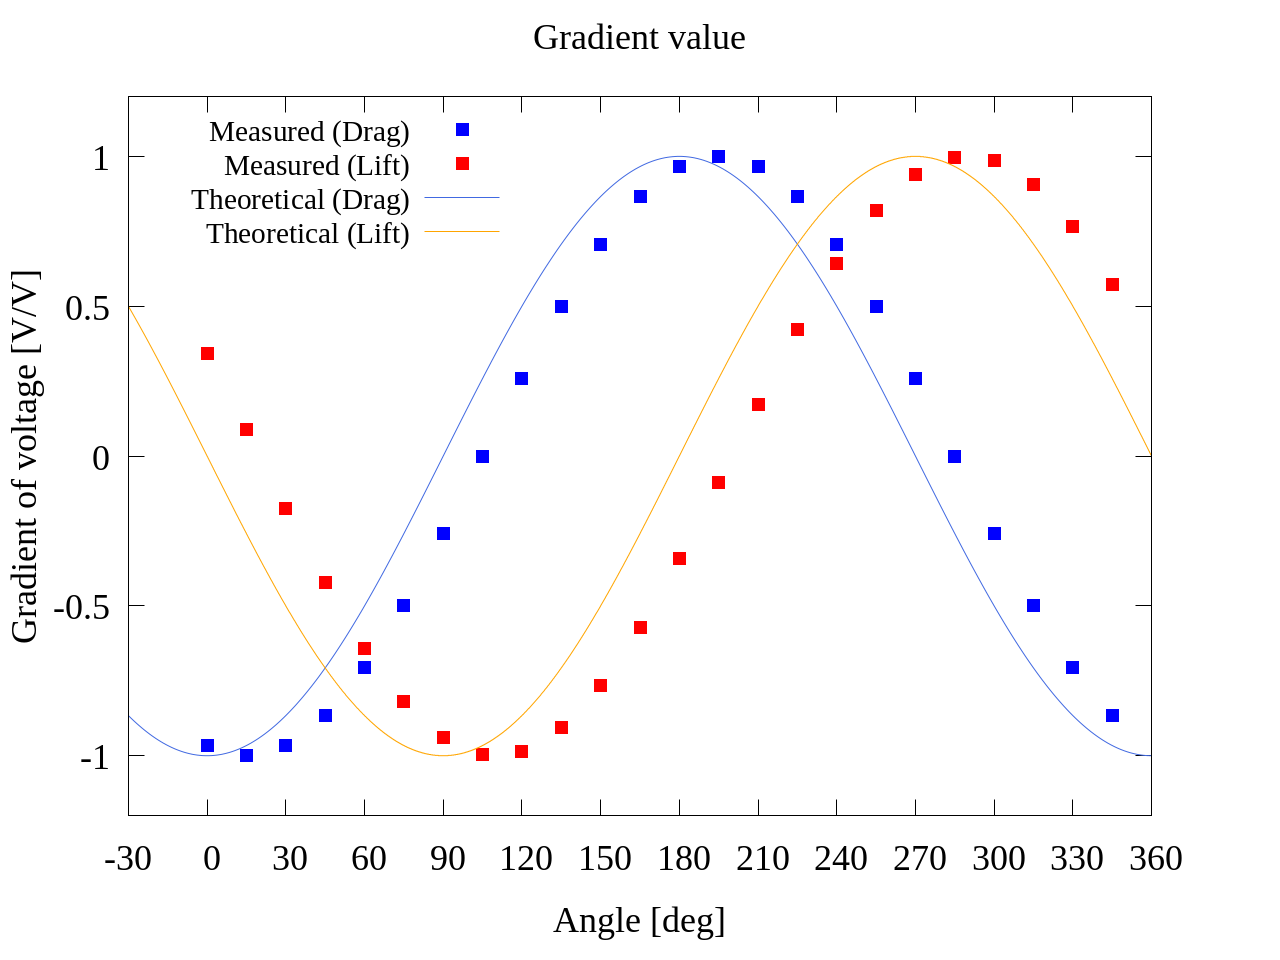
\includegraphics[width=95mm]{../../02_workspace/result/rotation_tx=15.0_tx=20.0/plot/20/20_adjust-value.png}
        \caption{Simulated data [Case 1]}
    \end{center}
\end{figure}

Fig.をみると,理論値の曲線とプロットされたテストデータに位相差があることがわかる.
このとき,テストデータに離散フーリ変換を適用すると波数1の成分について以下のTable のような値を得ることができる.
また,そのときのスペクトルを以下のFig. に示す.

\begin{table}[htbp]
    \begin{center}
        \caption{DFT result value [Case 1]}
        \begin{tabular}{|p{30mm}|p{20mm}|p{20mm}|}
            \hline
            \multicolumn{1}{|c|}{}     & \multicolumn{1}{|c|}{$Re$}    & \multicolumn{1}{|c|}{$Im$}   \\ \hline
            \multicolumn{1}{|c|}{Drag} & \multicolumn{1}{|c|}{-11.591} & \multicolumn{1}{|c|}{3.106}  \\ \hline
            \multicolumn{1}{|c|}{Lift} & \multicolumn{1}{|c|}{4.104}   & \multicolumn{1}{|c|}{11.276} \\ \hline
        \end{tabular}
    \end{center}
\end{table}

\begin{multicols}{2}
    \begin{figure_here}
        \begin{center}
            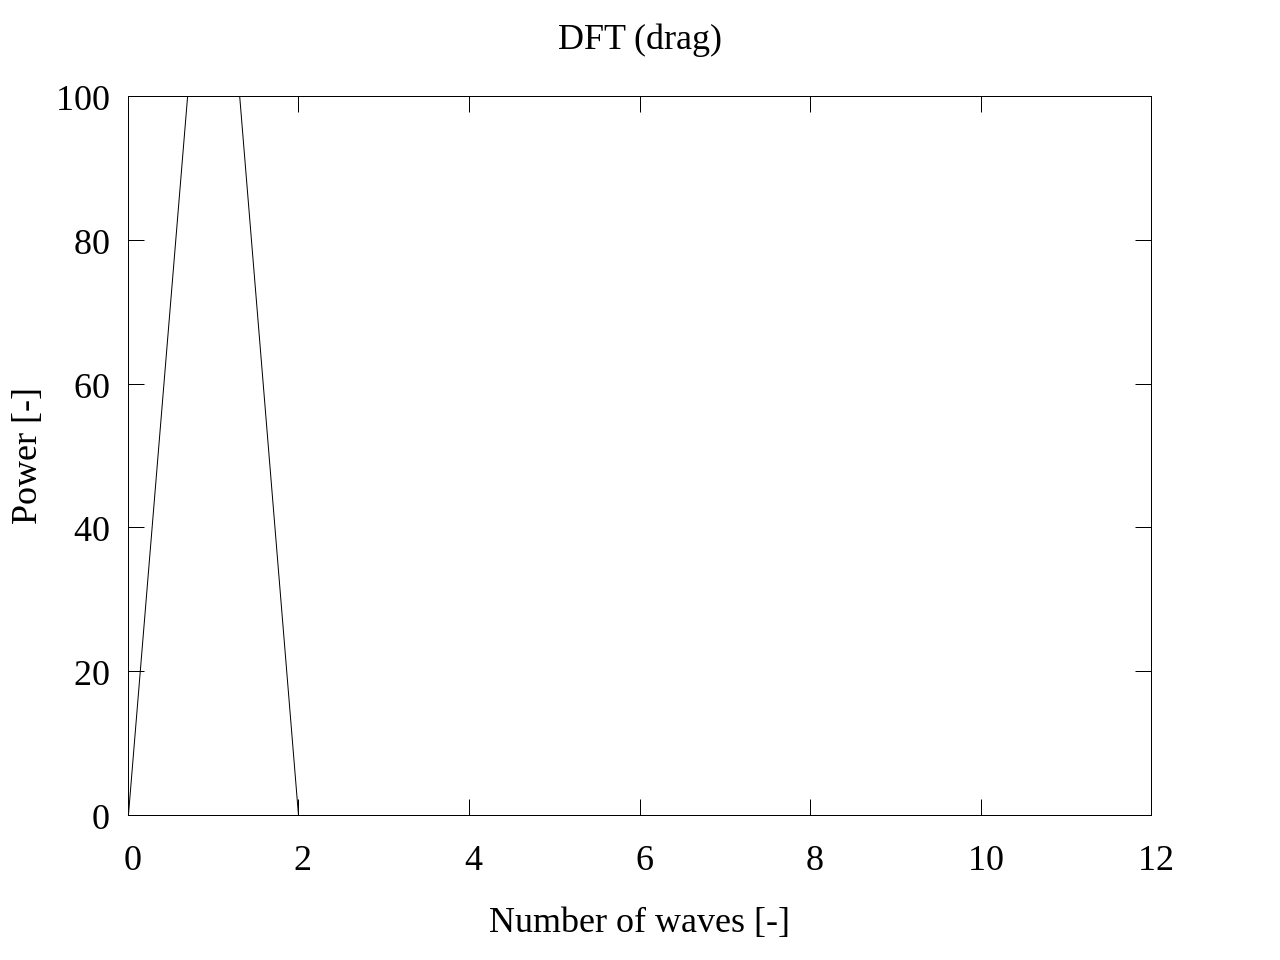
\includegraphics[width=65mm]{../../02_workspace/result/rotation_tx=15.0_tx=20.0/plot/07/07-3_dft-drag.png}
            \caption{DFT result (Drag) [Case 1]}
        \end{center}
    \end{figure_here}

    \begin{figure_here}
        \begin{center}
            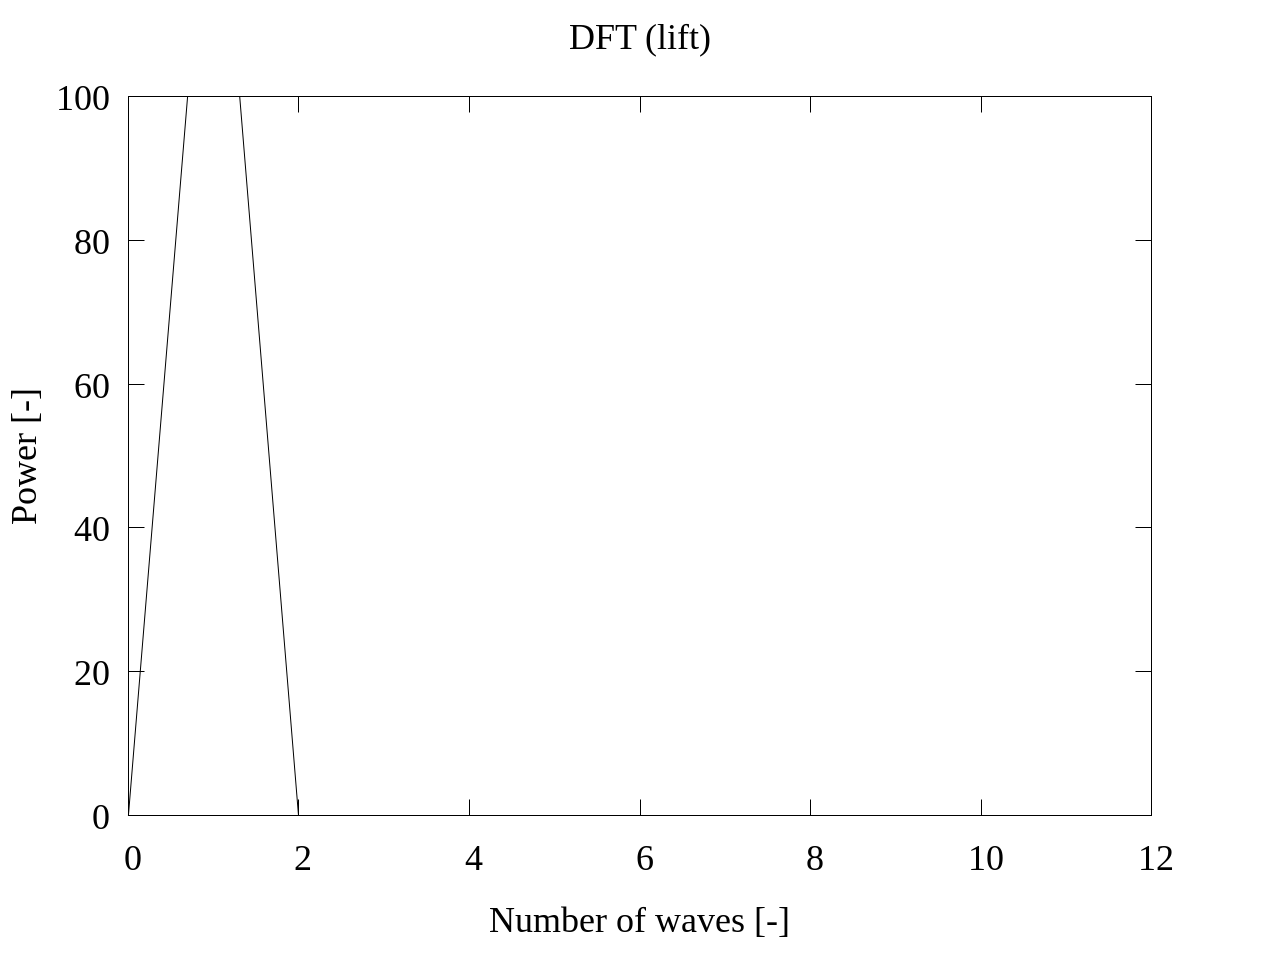
\includegraphics[width=65mm]{../../02_workspace/result/rotation_tx=15.0_tx=20.0/plot/07/07-4_dft-lift.png}
            \caption{DFT result (Lift) [Case 1]}
        \end{center}
    \end{figure_here}
\end{multicols}

Fig. ,Fig. より,波数1についてピークがあることがわかり,データの特徴を正しく捉えられているといえる.
ここで,Table について,式()より位相角$\phi_{1\;\mathrm{test}}$,$\phi_{2\;\mathrm{test}}$をそれぞれ算出する.

\begin{align}
    \phi_{1\;\mathrm{test}} & = \arctan \left(\frac{3.106}{-11.591} \right) \cdot \frac{180}{\pi} = 165.000 \;\mathrm{[deg]} \\
    \notag                                                                                                                   \\
    \phi_{2\;\mathrm{test}} & = \arctan \left(\frac{11.276}{4.101}\right) \cdot \frac{180}{\pi} = 70.000 \;\mathrm{[deg]}
\end{align}
\vskip \baselineskip

式(),式()より算出した位相角を用いて位相差$\theta_{1 \;\mathrm{test}}$,$\theta_{2 \;\mathrm{test}}$を求める.

\begin{align}
    \theta_{1\;\mathrm{test}} & = \pi \cdot \frac{180}{\pi} - 165.000 = 15.000\;\mathrm{[deg]}          \\
    \notag                                                                                              \\
    \theta_{2\;\mathrm{test}} & = \frac{\pi}{2} \cdot \frac{180}{\pi} - 70.000 = 20.000\;\mathrm{[deg]}
\end{align}
\vskip \baselineskip

また,位相差$\theta_{1 \;\mathrm{test}}$,$\theta_{2 \;\mathrm{test}}$より,
ひずみセンサの取付角$\phi_{s\;\mathrm{test}}$が式()よりわかる.

\begin{align}
    \phi_{s\;\mathrm{test}} = \left|15.000 - 20.000\right| = 5 \;[\mathrm{deg} ]
\end{align}

次に,位相差位相差$\theta_{1 \;\mathrm{test}}$,$\theta_{2 \;\mathrm{test}}$,
テストデータから得られる$v_{x'\;\mathrm{test}}$,$v_{xy\;\mathrm{test}}$より,
正規座標系における出力電圧勾配$v_x$,$v_y$を
式()を用いて算出する.それぞれの角度についての算出結果を以下のTable ,Fig. ,Fig. に示す.

\begin{table}[htbp]
    \begin{center}
        \caption{Corected result of test data [Case 1]}
        \begin{tabular}{|p{20mm}|p{20mm}|p{20mm}|p{20mm}|p{20mm}|}
            \hline
            \multicolumn{1}{|c|}{\textgt{Angle [deg]}} & \multicolumn{1}{|c|}{\textgt{$v_{x'\;\mathrm{test}}$ [V/V]}} & \multicolumn{1}{|c|}{\textgt{$v_{xy\;\mathrm{test}}$ [V/V]}} & \multicolumn{1}{|c|}{\textgt{$v_x$ [V/V]}} & \multicolumn{1}{|c|}{\textgt{$v_y$ [V/V]}} \\ \hline
            \multicolumn{1}{|c|}{0}                    & \multicolumn{1}{|r|}{-0.966}                                 & \multicolumn{1}{|r|}{0.342}                                  & \multicolumn{1}{|r|}{-1.000}               & \multicolumn{1}{|r|}{0.000}                \\ \hline
            \multicolumn{1}{|c|}{15}                   & \multicolumn{1}{|r|}{-1.000}                                 & \multicolumn{1}{|r|}{0.087}                                  & \multicolumn{1}{|r|}{-0.966}               & \multicolumn{1}{|r|}{-0.259}               \\ \hline
            \multicolumn{1}{|c|}{30}                   & \multicolumn{1}{|r|}{-0.966}                                 & \multicolumn{1}{|r|}{-0.174}                                 & \multicolumn{1}{|r|}{-0.866}               & \multicolumn{1}{|r|}{-0.500}               \\ \hline
            \multicolumn{1}{|c|}{45}                   & \multicolumn{1}{|r|}{-0.866}                                 & \multicolumn{1}{|r|}{-0.423}                                 & \multicolumn{1}{|r|}{-0.707}               & \multicolumn{1}{|r|}{-0.707}               \\ \hline
            \multicolumn{1}{|c|}{60}                   & \multicolumn{1}{|r|}{-0.707}                                 & \multicolumn{1}{|r|}{-0.643}                                 & \multicolumn{1}{|r|}{-0.500}               & \multicolumn{1}{|r|}{-0.866}               \\ \hline
            \multicolumn{1}{|c|}{75}                   & \multicolumn{1}{|r|}{-0.500}                                 & \multicolumn{1}{|r|}{-0.819}                                 & \multicolumn{1}{|r|}{-0.259}               & \multicolumn{1}{|r|}{-0.966}               \\ \hline
            \multicolumn{1}{|c|}{90}                   & \multicolumn{1}{|r|}{-0.259}                                 & \multicolumn{1}{|r|}{-0.940}                                 & \multicolumn{1}{|r|}{0.000}                & \multicolumn{1}{|r|}{-1.000}               \\ \hline
            \multicolumn{1}{|c|}{105}                  & \multicolumn{1}{|r|}{0.000}                                  & \multicolumn{1}{|r|}{-0.996}                                 & \multicolumn{1}{|r|}{0.259}                & \multicolumn{1}{|r|}{-0.966}               \\ \hline
            \multicolumn{1}{|c|}{120}                  & \multicolumn{1}{|r|}{0.259}                                  & \multicolumn{1}{|r|}{-0.985}                                 & \multicolumn{1}{|r|}{0.500}                & \multicolumn{1}{|r|}{-0.866}               \\ \hline
            \multicolumn{1}{|c|}{135}                  & \multicolumn{1}{|r|}{0.500}                                  & \multicolumn{1}{|r|}{-0.906}                                 & \multicolumn{1}{|r|}{0.707}                & \multicolumn{1}{|r|}{-0.707}               \\ \hline
            \multicolumn{1}{|c|}{150}                  & \multicolumn{1}{|r|}{0.707}                                  & \multicolumn{1}{|r|}{-0.766}                                 & \multicolumn{1}{|r|}{0.866}                & \multicolumn{1}{|r|}{-0.500}               \\ \hline
            \multicolumn{1}{|c|}{165}                  & \multicolumn{1}{|r|}{0.866}                                  & \multicolumn{1}{|r|}{-0.574}                                 & \multicolumn{1}{|r|}{0.966}                & \multicolumn{1}{|r|}{-0.259}               \\ \hline
            \multicolumn{1}{|c|}{180}                  & \multicolumn{1}{|r|}{0.966}                                  & \multicolumn{1}{|r|}{-0.342}                                 & \multicolumn{1}{|r|}{1.000}                & \multicolumn{1}{|r|}{-0.000}               \\ \hline
            \multicolumn{1}{|c|}{195}                  & \multicolumn{1}{|r|}{1.000}                                  & \multicolumn{1}{|r|}{-0.087}                                 & \multicolumn{1}{|r|}{0.966}                & \multicolumn{1}{|r|}{0.259}                \\ \hline
            \multicolumn{1}{|c|}{210}                  & \multicolumn{1}{|r|}{0.966}                                  & \multicolumn{1}{|r|}{0.174}                                  & \multicolumn{1}{|r|}{0.866}                & \multicolumn{1}{|r|}{0.500}                \\ \hline
            \multicolumn{1}{|c|}{225}                  & \multicolumn{1}{|r|}{0.866}                                  & \multicolumn{1}{|r|}{0.423}                                  & \multicolumn{1}{|r|}{0.707}                & \multicolumn{1}{|r|}{0.707}                \\ \hline
            \multicolumn{1}{|c|}{240}                  & \multicolumn{1}{|r|}{0.707}                                  & \multicolumn{1}{|r|}{0.643}                                  & \multicolumn{1}{|r|}{0.500}                & \multicolumn{1}{|r|}{0.866}                \\ \hline
            \multicolumn{1}{|c|}{255}                  & \multicolumn{1}{|r|}{0.500}                                  & \multicolumn{1}{|r|}{0.819}                                  & \multicolumn{1}{|r|}{0.259}                & \multicolumn{1}{|r|}{0.966}                \\ \hline
            \multicolumn{1}{|c|}{270}                  & \multicolumn{1}{|r|}{0.259}                                  & \multicolumn{1}{|r|}{0.940}                                  & \multicolumn{1}{|r|}{-0.000}               & \multicolumn{1}{|r|}{1.000}                \\ \hline
            \multicolumn{1}{|c|}{285}                  & \multicolumn{1}{|r|}{-0.000}                                 & \multicolumn{1}{|r|}{0.996}                                  & \multicolumn{1}{|r|}{-0.259}               & \multicolumn{1}{|r|}{0.966}                \\ \hline
            \multicolumn{1}{|c|}{300}                  & \multicolumn{1}{|r|}{-0.259}                                 & \multicolumn{1}{|r|}{0.985}                                  & \multicolumn{1}{|r|}{-0.500}               & \multicolumn{1}{|r|}{0.866}                \\ \hline
            \multicolumn{1}{|c|}{315}                  & \multicolumn{1}{|r|}{-0.500}                                 & \multicolumn{1}{|r|}{0.906}                                  & \multicolumn{1}{|r|}{-0.707}               & \multicolumn{1}{|r|}{0.707}                \\ \hline
            \multicolumn{1}{|c|}{330}                  & \multicolumn{1}{|r|}{-0.707}                                 & \multicolumn{1}{|r|}{0.766}                                  & \multicolumn{1}{|r|}{-0.866}               & \multicolumn{1}{|r|}{0.500}                \\ \hline
            \multicolumn{1}{|c|}{345}                  & \multicolumn{1}{|r|}{-0.866}                                 & \multicolumn{1}{|r|}{0.574}                                  & \multicolumn{1}{|r|}{-0.966}               & \multicolumn{1}{|r|}{0.259}                \\ \hline
        \end{tabular}
    \end{center}
\end{table}

\begin{figure}
    \footnotesize
    \begin{center}
        \includegraphics[width=95mm]{../../02_workspace/result/rotation_tx=15.0_tx=20.0/plot/21/21-4_corrected_angle_drag.png}
        \caption{Corrected data (Drag) [Case 1]}
        \includegraphics[width=95mm]{../../02_workspace/result/rotation_tx=15.0_tx=20.0/plot/21/21-4_corrected_angle_lift.png}
        \caption{Corrected data (Lift) [Case 1]}
    \end{center}
\end{figure}

\newpage

Fig.,Fig.をみると算出された補正値すなわち正規座標系における出力電圧勾配は,
理論曲線状に位置していることが確認でき,正しく算出されていることがわかる.

\newpage
また,以下のFig.~Fig.に,Case2 および Case3 におけるテストデータとその補正結果について示す.

\begin{multicols}{2}
    \begin{figure_here}
        \subsubsection{テストデータ : Case 2}
        \vskip \baselineskip
        $\theta_{1 \mathrm{test}} = -15 \; \mathrm{[deg]}$, $\theta_{2 \mathrm{test}} = -20 \; \mathrm{[deg]}$
        \footnotesize
        \begin{center}
            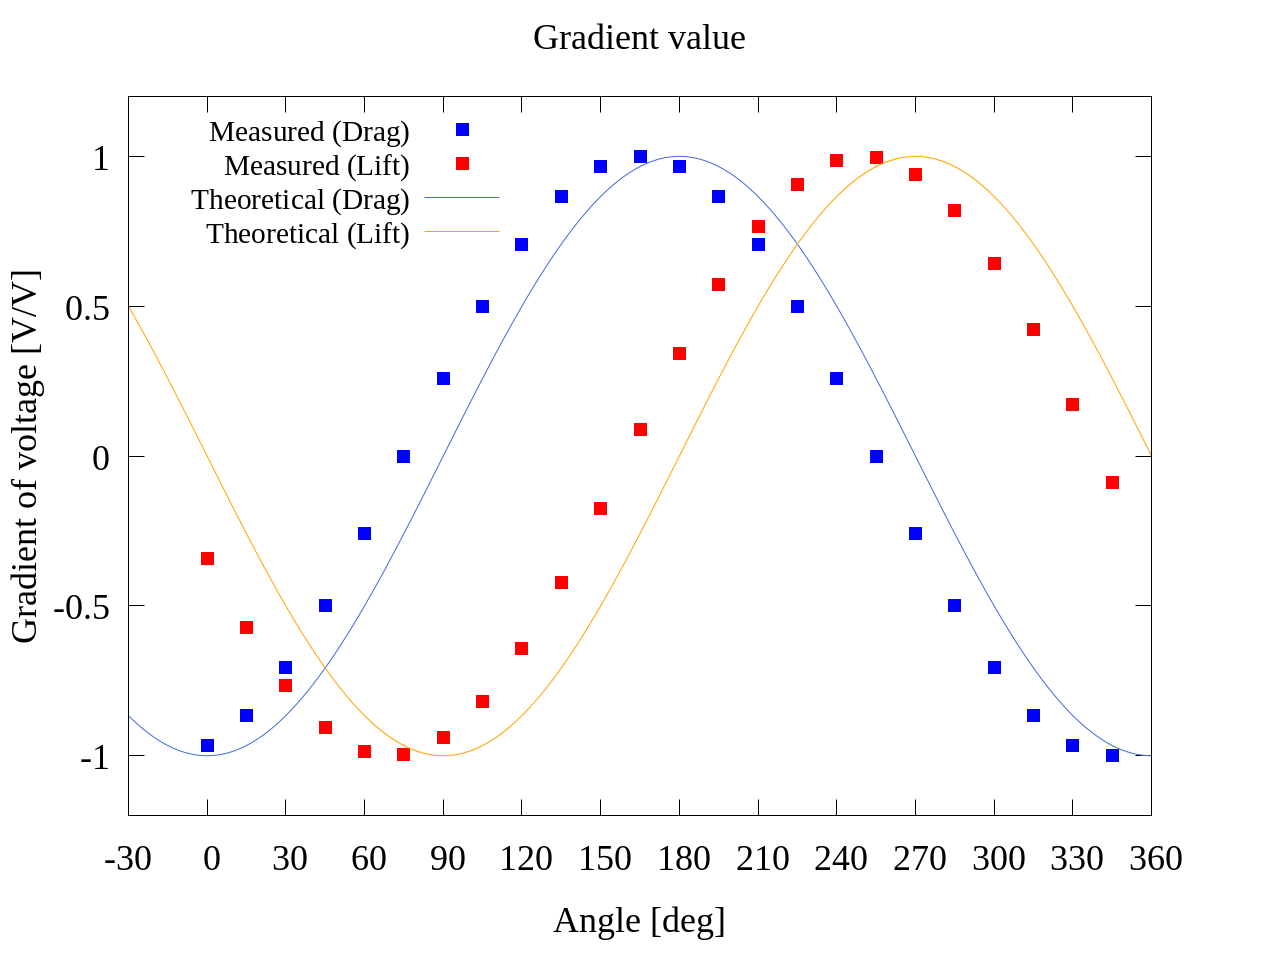
\includegraphics[width=65mm]{../../02_workspace/result/rotation_tx=-15.0_tx=-20.0/plot/20/20_adjust-value.png}
            \caption{Simulated data [Case 2]}
            \includegraphics[width=65mm]{../../02_workspace/result/rotation_tx=-15.0_tx=-20.0/plot/21/21-4_corrected_angle_drag.png}
            \caption{Corrected data (Drag) [Case 2]}
            \includegraphics[width=65mm]{../../02_workspace/result/rotation_tx=-15.0_tx=-20.0/plot/21/21-4_corrected_angle_lift.png}
            \caption{Corrected data (Lift) [Case 2]}
        \end{center}
    \end{figure_here}

    \begin{figure_here}
        \subsubsection{テストデータ : Case 3}
        \vskip \baselineskip
        $\theta_{1 \mathrm{test}} = 90 \; \mathrm{[deg]}$, $\theta_{2 \mathrm{test}} = -90 \; \mathrm{[deg]}$
        \footnotesize
        \begin{center}
            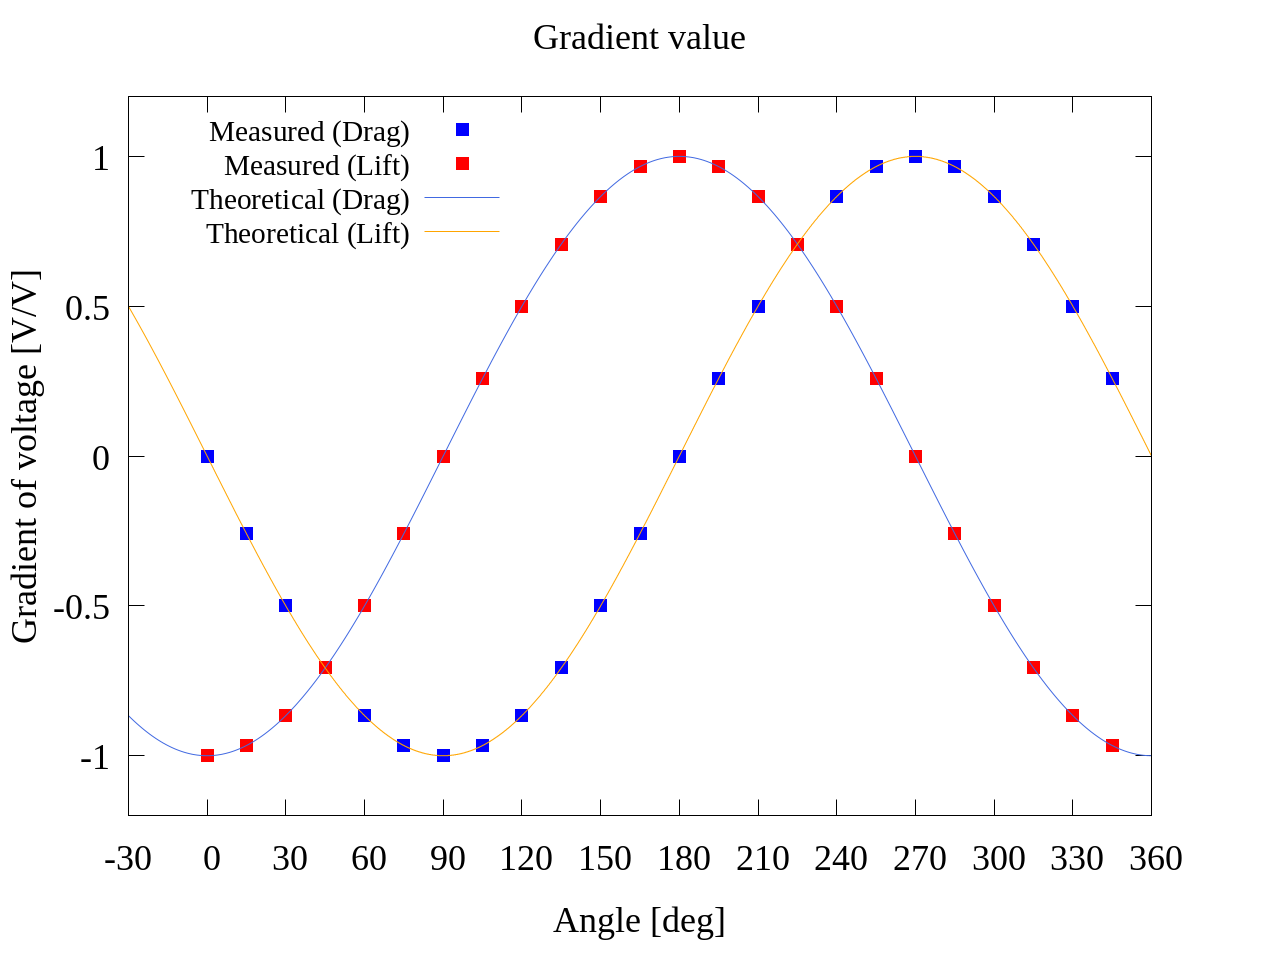
\includegraphics[width=65mm]{../../02_workspace/result/rotation_tx=90.0_tx=-90.0/plot/20/20_adjust-value.png}
            \caption{Simulated data [Case 3]}
            \includegraphics[width=65mm]{../../02_workspace/result/rotation_tx=90.0_tx=-90.0/plot/21/21-4_corrected_angle_drag.png}
            \caption{Corrected data (Drag) [Case 3]}
            \includegraphics[width=65mm]{../../02_workspace/result/rotation_tx=90.0_tx=-90.0/plot/21/21-4_corrected_angle_lift.png}
            \caption{Corrected data (Lift) [Case 3]}
        \end{center}
    \end{figure_here}
\end{multicols}

ここで,Fig.~Fig.をみると回転角度が負の値の場合,その値が非常に大きい場合であっても
問題なく補正処理が可能であることがわかる.
したがって,座標系の回転における補正理論はテストデータについて正しく機能しており
正規座標系と座標系[1]の回転角および作用力測定装置のひずみセンサの取付角,
正規座標系における出力電圧勾配を調べることができる.

\subsection{座標系のオフセットにおける補正理論}

次に,正規座標系と座標系[2]のオフセットの補正理論を説明する.
ここでは,回転角はない($\theta_x = 0$,$\theta_2 = 0$)として考える.
正規座標系と座標系[2]の中心との位置関係にオフセット$\Delta x$,$\Delta y$を持つ.
ここで,作用力$F$を与えるとき,その作用線はオフセット$\Delta x$,$\Delta y$によって
正規座標系の中心$o$を通ることはなく,座標系[2]の中心$o''$を通る.
このとき,作用点と点$o''$を通る直線(青点線)と$x''$軸の角度を$\theta$,
作用点と点$o$を通る直線(赤点線)と$x$軸の角度を$\varphi$とする.
また,作用点と点$o'$を通る直線(青点線)と作用点と点$o$を通る直線(赤点線)の角度を$\alpha$とする.
角度$\theta$は校正実験時に記録される角度となる.

\begin{figure}[htbp]
    \footnotesize
    \begin{center}
        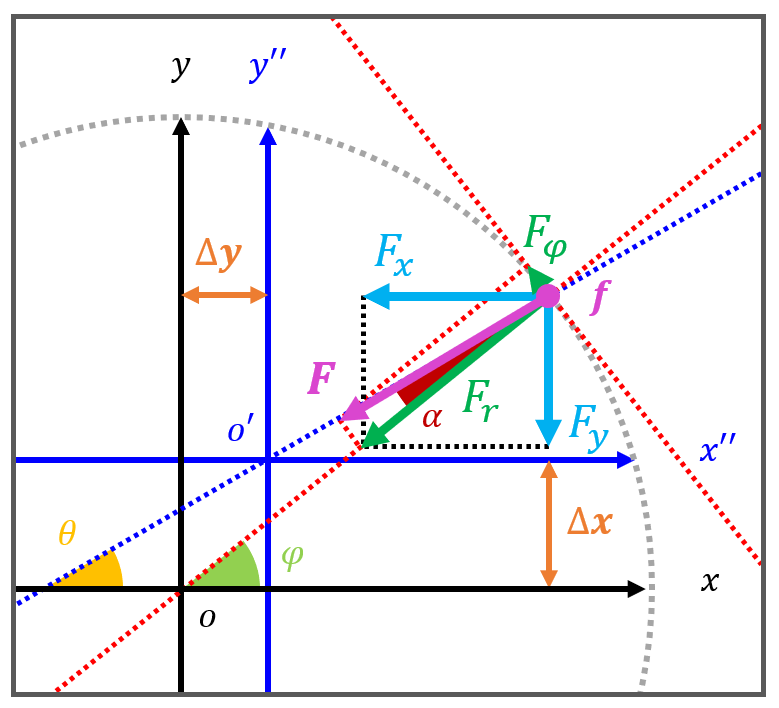
\includegraphics[width=75mm]{images/34-1.png}
        \caption{}
    \end{center}
\end{figure}

\subsubsection{角度$\alpha$の算出}
供試体の半径を$r$とするとき,作用点$F(x,y)$の座標は角度$\varphi$を用いて以下のように表すことができる.

\begin{align}
    x & = r \cos \varphi \\
    y & = r \sin \varphi
\end{align}
\vskip \baselineskip

また,座標系[2]において,作用点$F(x'',y'')$の座標はオフセット$\Delta x$,$\Delta y$を用いて
以下のように表される.

\begin{align}
    x'' & = r \cos \varphi -\Delta x \\
    y'' & = r \sin \varphi -\Delta y
\end{align}
\vskip \baselineskip

以上より,角度$\theta$を用いて角度$\varphi$を求めることができる.

\begin{align}
    \tan \theta & = \frac{y''}{x''} = \frac{ r \sin \varphi - \Delta y}{ r \cos \varphi - \Delta x}      \\
    \notag                                                                                               \\
    \varphi     & = \theta - \sin^{-1}\left(\frac{\Delta x \sin \theta - \Delta y \cos \theta}{r}\right)
\end{align}
\vskip \baselineskip

したがって,角度$\alpha$を以下のように求めることができる.

\begin{align}
    \alpha = \theta - \varphi = \sin^{-1} \left( \frac{\Delta x \sin \theta - \Delta y \cos \theta}{r} \right)
\end{align}
\vskip \baselineskip

\subsubsection{作用力$F$の分解}

供試体に加わる作用力$F$は供試体表面の接線方向の力$F_\varphi$,
またその法線方向の力$F_r$に分けて考えることができる.
ロードセルから与える作用力の角度$\theta$,算出した$\varphi$を用いると,それぞれ以下のように求められる.

\begin{align}
    F_{\varphi} & = F \sin \alpha \\
    F_{r}       & = F \cos \alpha
\end{align}
\vskip \baselineskip

供試体への作用力について抗力方向を$F_{x}$,揚力方向を$F_{y}$とすると
角度$\varphi$を用いて以下のように求められる.

\begin{align}
    F_{x} & = - F_r \cos \varphi \\
    F_{y} & = - F_r \sin \varphi
\end{align}
\vskip \baselineskip

また,接線方向成分$F_\varphi$について,供試体に対してトルク$T$として作用することとなる.

\begin{align}
    T & = F_\varphi \cdot r = F \sin \alpha \cdot r
\end{align}
\vskip \baselineskip

ここで,このトルク$T$について,
作用力測定装置に対する影響は十分に小さいと考えられることから無視できる.\\

\subsubsection{出力電圧勾配の座標系変換 (2)}

正規座標系に対して,オフセットを持つ座標系[2]を基準に
ロードセルから与えられる作用力$F$はすべて供試体に伝わることはなく,
接線方向の力$F_r$,その法線方向の力$F_\theta$に分解される.
すなわち,測定時にはロードセルから作用力$F$を与えた際の出力電圧,
ひずみセンサから作用力$F_r$を与えた際の出力電圧を得ているということになる.
したがって,ひずみセンサの出力電圧の傾きを一様に評価することは不可能であり,
実際の作用力$F_r$の角度$\alpha$を算出し補正を加える必要がある.

ここで,ひずみセンサの出力電圧$V_{x''2}$,$V_{y''2}$は
それぞれ$F_r / F$倍されていると考えられることから,
正規座標系における出力電圧勾配$v_{x}$,$v_{y}$と
座標系[2]における出力電圧勾配$v_{x''2}$,$v_{y''2}$は
角度$\alpha$を用いて以下のような関係が成立する.

\begin{align}
    v_{x} & = \frac{F}{F_r} v_{x''2} = \frac{1}{\cos \alpha} v_{x''2} \\
    \notag                                                            \\
    v_{y} & = \frac{F}{F_r} v_{y''2} = \frac{1}{\cos \alpha} v_{y''2}
\end{align}

\subsubsection{補正理論のテストデータへの適用 (2)}

以上の補正理論より,オフセットを考慮したテストデータを作成する.
任意のオフセット$\Delta x_\mathrm{test}$,$\Delta y_\mathrm{test}$を与えて
座標系[2]の出力電圧勾配について,$x''$軸方向を$v_{x''\;\mathrm{test}}$,
$y''$軸方向を$v_{y''\;\mathrm{test}}$とするとき,以下のように表される.

\begin{align}
    \theta                  & = \frac{\pi}{180} \; i \;\left(i = 0, 1, 2, 3, \cdots\right)                                                       \\
    \alpha                  & = \sin^{-1} \left( \frac{\Delta x_\mathrm{test} \sin \theta - \Delta y_\mathrm{test} \cos \theta}{r} \right)       \\
    \varphi                 & = \theta - \sin^{-1}\left(\frac{\Delta x_\mathrm{test} \sin \theta - \Delta y_\mathrm{test} \cos \theta}{r}\right) \\
    v_{x'' \;\mathrm{test}} & = - \cos \alpha \cos \varphi                                                                                       \\
    v_{y'' \;\mathrm{test}} & = - \cos \alpha \sin \varphi
\end{align}
\vskip \baselineskip

また,今回を以下のTable のようなパラメータを用いた.

\begin{table}[htbp]
    \begin{center}
        \caption{Test data conditions (2)}
        \begin{tabular}{|p{30mm}|p{20mm}|p{20mm}|}
            \hline
            \multicolumn{1}{|c|}{}       & \multicolumn{1}{|c|}{$\Delta x_\mathrm{test}$ [mm]} & \multicolumn{1}{|c|}{$\Delta y_\mathrm{test}$ [mm]} \\ \hline
            \multicolumn{1}{|c|}{Case 4} & \multicolumn{1}{|c|}{5.0}                           & \multicolumn{1}{|c|}{0.0}                           \\ \hline
            \multicolumn{1}{|c|}{Case 5} & \multicolumn{1}{|c|}{5.0}                           & \multicolumn{1}{|c|}{-5.0}                          \\ \hline
            \multicolumn{1}{|c|}{Case 6} & \multicolumn{1}{|c|}{10.0}                          & \multicolumn{1}{|c|}{-5.0}                          \\ \hline
        \end{tabular}
    \end{center}
\end{table}

ここで,Case 4 に対する座標系の回転おける補正理論の適用過程について説明する.
はじめに,作成したテストデータを以下に示す.

\begin{figure}[htbp]
    \footnotesize
    \begin{center}
        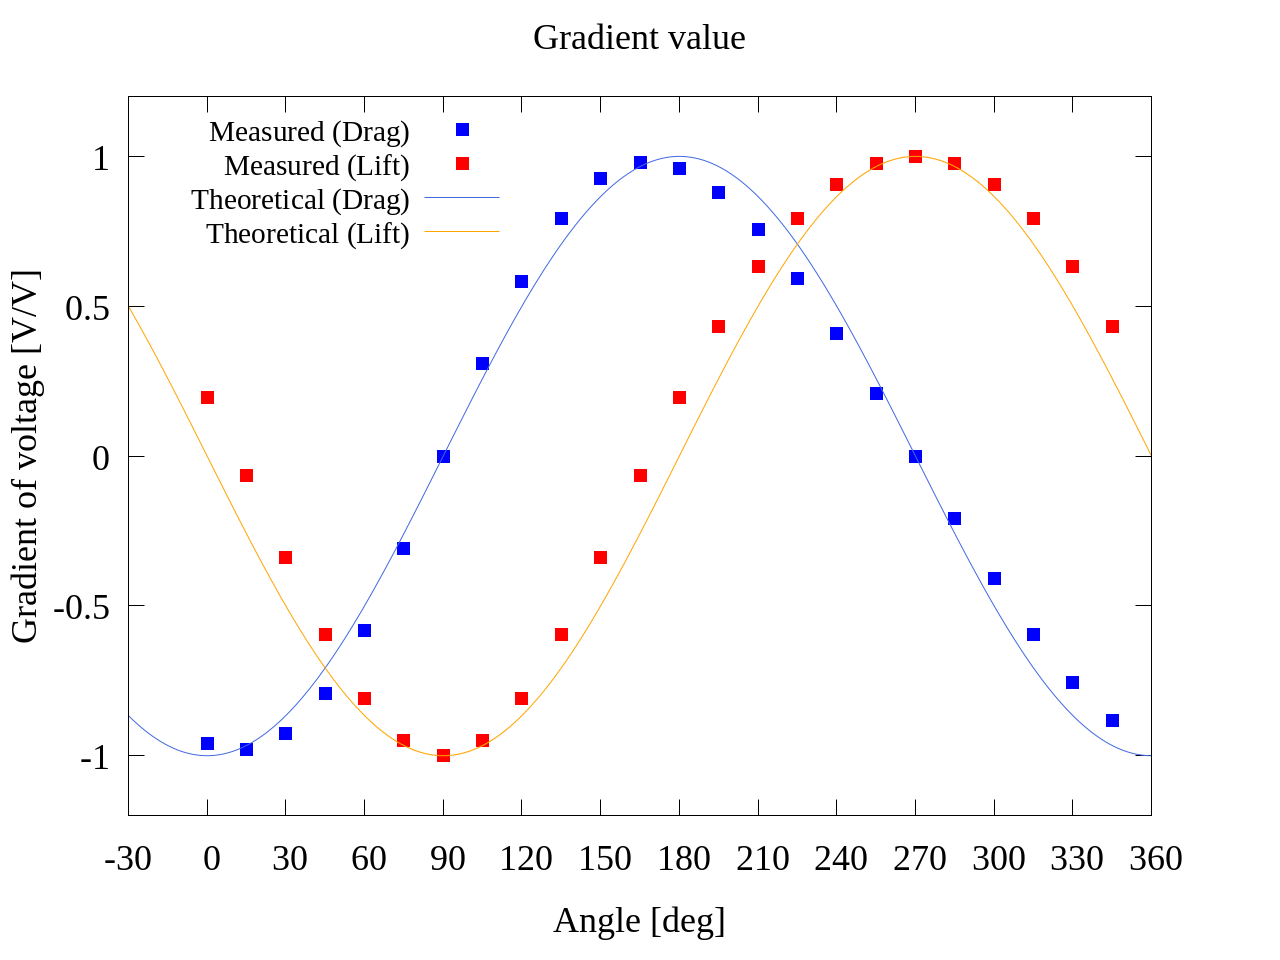
\includegraphics[width=95mm]{../../02_workspace/result/offset_dx=5.0_dy=0.0/plot/20/20_adjust-value.png}
        \caption{Simulated data [Case 4]}
    \end{center}
\end{figure}
\vskip \baselineskip

Fig.をみると,プロットされたテストデータは理論値の曲線とは異なる値を示している.
また,波形は少し不規則な形状となっていることがわかる.

\newpage

ここで,$\theta$,$\Delta x_\mathrm{test}$,$\Delta y_\mathrm{test}$は既知の変数であるため
式()より,$\alpha$および$\varphi$を求めることができる.
したがって,式()を適用した結果を以下のTable に示す.
ここで,$\varphi$は正規座標系において供試体へ作用力が加えられている角度を示していることになる.

\begin{table}[htbp]
    \begin{center}
        \caption{Corected result of test data [Case 4]}
        \begin{tabular}{|p{15 mm}|p{15 mm}|p{15 mm}|p{15 mm}|p{15 mm}|p{15 mm}|}
            \hline
            \multicolumn{1}{|c|}{\textgt{Angle [deg]}} & \multicolumn{1}{|c|}{\textgt{$v_{x''\;\mathrm{test}}$ [V/V]}} & \multicolumn{1}{|c|}{\textgt{$v_{y''\;\mathrm{test}}$ [V/V]}} & \multicolumn{1}{|c|}{\textgt{$v_x$ [V/V]}} & \multicolumn{1}{|c|}{\textgt{$v_y$ [V/V]}} & \multicolumn{1}{|c|}{\textgt{$\varphi$ [deg]}} \\ \hline
            \multicolumn{1}{|c|}{0}                    & \multicolumn{1}{|r|}{-0.960}                                  & \multicolumn{1}{|r|}{0.196}                                   & \multicolumn{1}{|r|}{-0.980}               & \multicolumn{1}{|r|}{0.200}                & \multicolumn{1}{|r|}{-11.5}                    \\ \hline
            \multicolumn{1}{|c|}{15}                   & \multicolumn{1}{|r|}{-0.979}                                  & \multicolumn{1}{|r|}{-0.066}                                  & \multicolumn{1}{|r|}{-0.998}               & \multicolumn{1}{|r|}{-0.067}               & \multicolumn{1}{|r|}{3.9}                      \\ \hline
            \multicolumn{1}{|c|}{30}                   & \multicolumn{1}{|r|}{-0.925}                                  & \multicolumn{1}{|r|}{-0.337}                                  & \multicolumn{1}{|r|}{-0.940}               & \multicolumn{1}{|r|}{-0.342}               & \multicolumn{1}{|r|}{20.0}                     \\ \hline
            \multicolumn{1}{|c|}{45}                   & \multicolumn{1}{|r|}{-0.792}                                  & \multicolumn{1}{|r|}{-0.594}                                  & \multicolumn{1}{|r|}{-0.800}               & \multicolumn{1}{|r|}{-0.600}               & \multicolumn{1}{|r|}{36.9}                     \\ \hline
            \multicolumn{1}{|c|}{60}                   & \multicolumn{1}{|r|}{-0.581}                                  & \multicolumn{1}{|r|}{-0.808}                                  & \multicolumn{1}{|r|}{-0.584}               & \multicolumn{1}{|r|}{-0.812}               & \multicolumn{1}{|r|}{54.3}                     \\ \hline
            \multicolumn{1}{|c|}{75}                   & \multicolumn{1}{|r|}{-0.308}                                  & \multicolumn{1}{|r|}{-0.950}                                  & \multicolumn{1}{|r|}{-0.308}               & \multicolumn{1}{|r|}{-0.951}               & \multicolumn{1}{|r|}{72.0}                     \\ \hline
            \multicolumn{1}{|c|}{90}                   & \multicolumn{1}{|r|}{-0.000}                                  & \multicolumn{1}{|r|}{-1.000}                                  & \multicolumn{1}{|r|}{-0.000}               & \multicolumn{1}{|r|}{-1.000}               & \multicolumn{1}{|r|}{90.0}                     \\ \hline
            \multicolumn{1}{|c|}{105}                  & \multicolumn{1}{|r|}{0.308}                                   & \multicolumn{1}{|r|}{-0.950}                                  & \multicolumn{1}{|r|}{0.308}                & \multicolumn{1}{|r|}{-0.951}               & \multicolumn{1}{|r|}{108.0}                    \\ \hline
            \multicolumn{1}{|c|}{120}                  & \multicolumn{1}{|r|}{0.581}                                   & \multicolumn{1}{|r|}{-0.808}                                  & \multicolumn{1}{|r|}{0.584}                & \multicolumn{1}{|r|}{-0.812}               & \multicolumn{1}{|r|}{125.7}                    \\ \hline
            \multicolumn{1}{|c|}{135}                  & \multicolumn{1}{|r|}{0.792}                                   & \multicolumn{1}{|r|}{-0.594}                                  & \multicolumn{1}{|r|}{0.800}                & \multicolumn{1}{|r|}{-0.600}               & \multicolumn{1}{|r|}{143.1}                    \\ \hline
            \multicolumn{1}{|c|}{150}                  & \multicolumn{1}{|r|}{0.925}                                   & \multicolumn{1}{|r|}{-0.337}                                  & \multicolumn{1}{|r|}{0.940}                & \multicolumn{1}{|r|}{-0.342}               & \multicolumn{1}{|r|}{160.0}                    \\ \hline
            \multicolumn{1}{|c|}{165}                  & \multicolumn{1}{|r|}{0.979}                                   & \multicolumn{1}{|r|}{-0.066}                                  & \multicolumn{1}{|r|}{0.998}                & \multicolumn{1}{|r|}{-0.067}               & \multicolumn{1}{|r|}{176.1}                    \\ \hline
            \multicolumn{1}{|c|}{180}                  & \multicolumn{1}{|r|}{0.960}                                   & \multicolumn{1}{|r|}{0.196}                                   & \multicolumn{1}{|r|}{0.980}                & \multicolumn{1}{|r|}{0.200}                & \multicolumn{1}{|r|}{191.5}                    \\ \hline
            \multicolumn{1}{|c|}{195}                  & \multicolumn{1}{|r|}{0.881}                                   & \multicolumn{1}{|r|}{0.432}                                   & \multicolumn{1}{|r|}{0.898}                & \multicolumn{1}{|r|}{0.441}                & \multicolumn{1}{|r|}{206.1}                    \\ \hline
            \multicolumn{1}{|c|}{210}                  & \multicolumn{1}{|r|}{0.755}                                   & \multicolumn{1}{|r|}{0.632}                                   & \multicolumn{1}{|r|}{0.766}                & \multicolumn{1}{|r|}{0.642}                & \multicolumn{1}{|r|}{220.0}                    \\ \hline
            \multicolumn{1}{|c|}{225}                  & \multicolumn{1}{|r|}{0.594}                                   & \multicolumn{1}{|r|}{0.792}                                   & \multicolumn{1}{|r|}{0.600}                & \multicolumn{1}{|r|}{0.800}                & \multicolumn{1}{|r|}{233.1}                    \\ \hline
            \multicolumn{1}{|c|}{240}                  & \multicolumn{1}{|r|}{0.409}                                   & \multicolumn{1}{|r|}{0.907}                                   & \multicolumn{1}{|r|}{0.411}                & \multicolumn{1}{|r|}{0.912}                & \multicolumn{1}{|r|}{245.7}                    \\ \hline
            \multicolumn{1}{|c|}{255}                  & \multicolumn{1}{|r|}{0.208}                                   & \multicolumn{1}{|r|}{0.977}                                   & \multicolumn{1}{|r|}{0.208}                & \multicolumn{1}{|r|}{0.978}                & \multicolumn{1}{|r|}{258.0}                    \\ \hline
            \multicolumn{1}{|c|}{270}                  & \multicolumn{1}{|r|}{0.000}                                   & \multicolumn{1}{|r|}{1.000}                                   & \multicolumn{1}{|r|}{0.000}                & \multicolumn{1}{|r|}{1.000}                & \multicolumn{1}{|r|}{270.0}                    \\ \hline
            \multicolumn{1}{|c|}{285}                  & \multicolumn{1}{|r|}{-0.208}                                  & \multicolumn{1}{|r|}{0.977}                                   & \multicolumn{1}{|r|}{-0.208}               & \multicolumn{1}{|r|}{0.978}                & \multicolumn{1}{|r|}{282.0}                    \\ \hline
            \multicolumn{1}{|c|}{300}                  & \multicolumn{1}{|r|}{-0.409}                                  & \multicolumn{1}{|r|}{0.907}                                   & \multicolumn{1}{|r|}{-0.411}               & \multicolumn{1}{|r|}{0.912}                & \multicolumn{1}{|r|}{294.3}                    \\ \hline
            \multicolumn{1}{|c|}{315}                  & \multicolumn{1}{|r|}{-0.594}                                  & \multicolumn{1}{|r|}{0.792}                                   & \multicolumn{1}{|r|}{-0.600}               & \multicolumn{1}{|r|}{0.800}                & \multicolumn{1}{|r|}{306.9}                    \\ \hline
            \multicolumn{1}{|c|}{330}                  & \multicolumn{1}{|r|}{-0.755}                                  & \multicolumn{1}{|r|}{0.633}                                   & \multicolumn{1}{|r|}{-0.766}               & \multicolumn{1}{|r|}{0.642}                & \multicolumn{1}{|r|}{320.0}                    \\ \hline
            \multicolumn{1}{|c|}{345}                  & \multicolumn{1}{|r|}{-0.881}                                  & \multicolumn{1}{|r|}{0.432}                                   & \multicolumn{1}{|r|}{-0.898}               & \multicolumn{1}{|r|}{0.441}                & \multicolumn{1}{|r|}{333.9}                    \\ \hline
        \end{tabular}
    \end{center}
\end{table}

\newpage

\begin{figure}[htbp]
    \footnotesize
    \begin{center}
        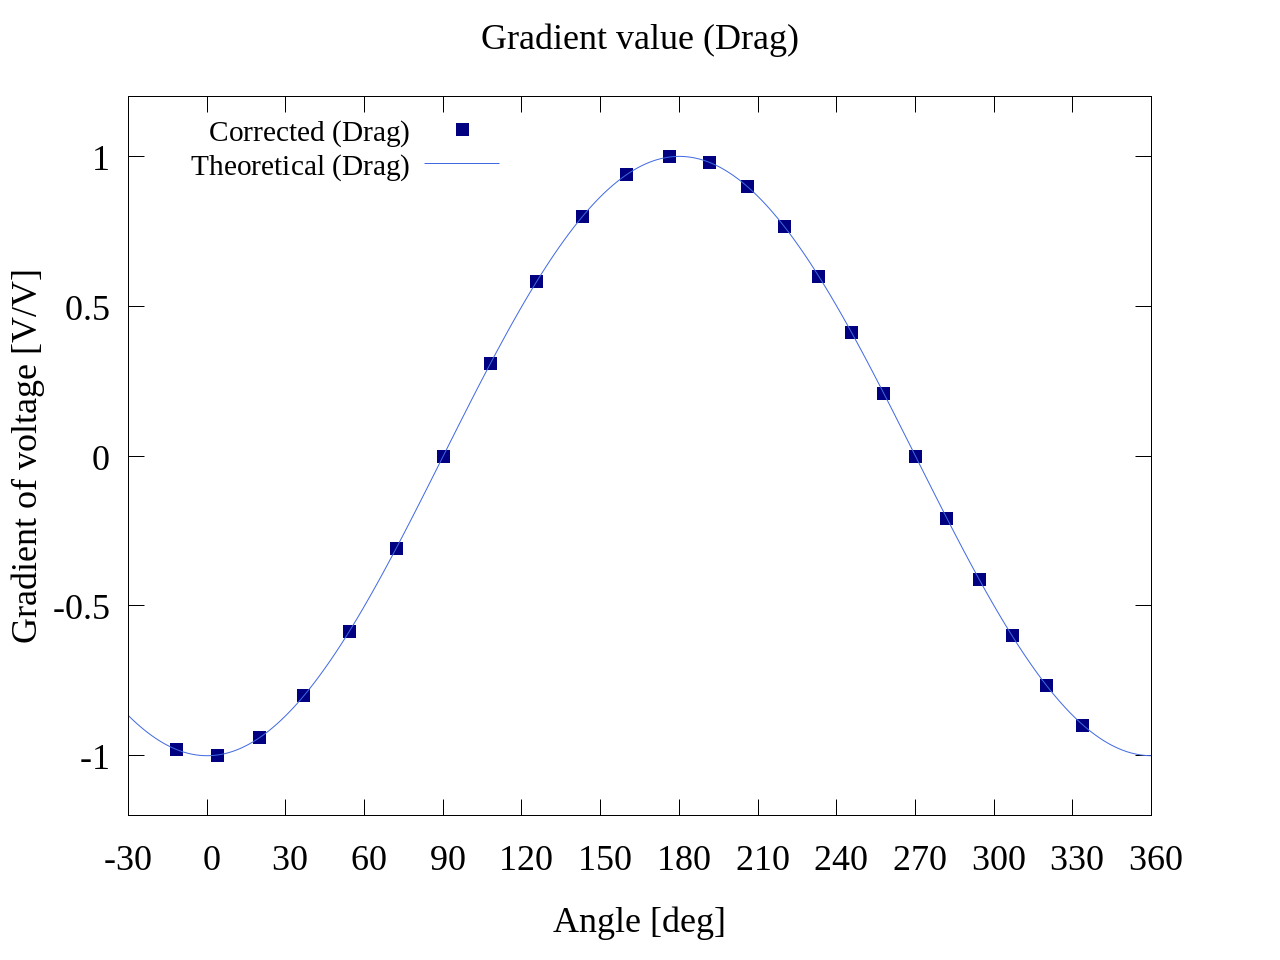
\includegraphics[width=95mm]{../../02_workspace/result/offset_dx=5.0_dy=0.0/plot/21/21-2_corrected_offset_drag.png}
        \caption{Corrected data (Drag) [Case 4]}
        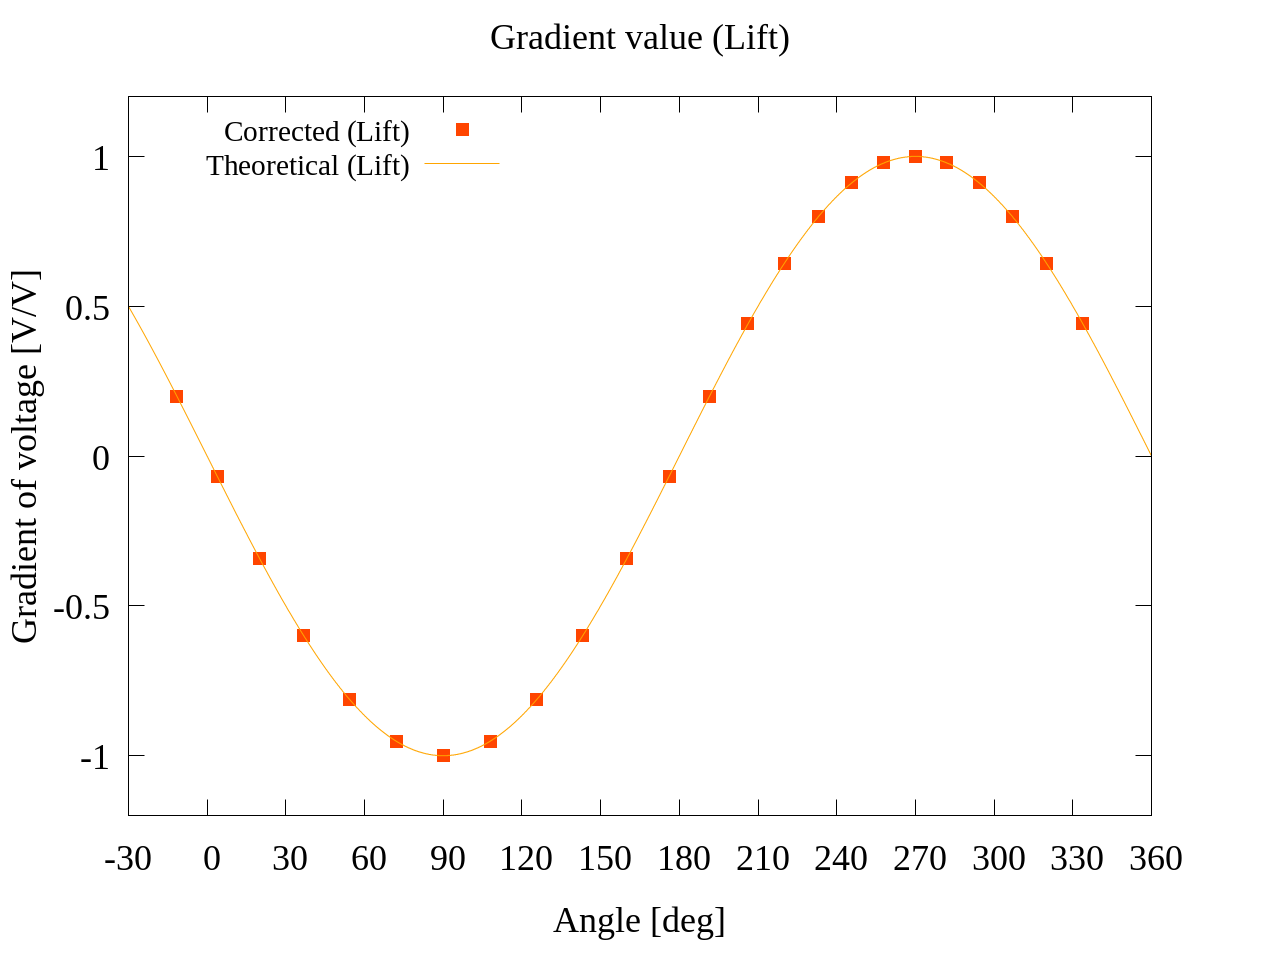
\includegraphics[width=95mm]{../../02_workspace/result/offset_dx=5.0_dy=0.0/plot/21/21-2_corrected_offset_lift.png}
        \caption{Corrected data (Lift) [Case 4]}
    \end{center}
\end{figure}


Fig.,Fig.をみると算出された補正値は理論曲線上に位置していることがわかる.
しかし,プロットされているデータの角度は$\varphi$となるため,不等間隔となってしまう.

\newpage
また,以下のFig.~Fig.に,Case 5 および Case 6 におけるテストデータとその補正結果について示す.

\begin{multicols}{2}
    \begin{figure_here}
        \subsubsection{テストデータ : Case 5}
        \vskip \baselineskip
        $\Delta x_\mathrm{test} = 5.0$ [mm],$\Delta x_\mathrm{test} = -5.0$ [mm]
        \footnotesize
        \begin{center}
            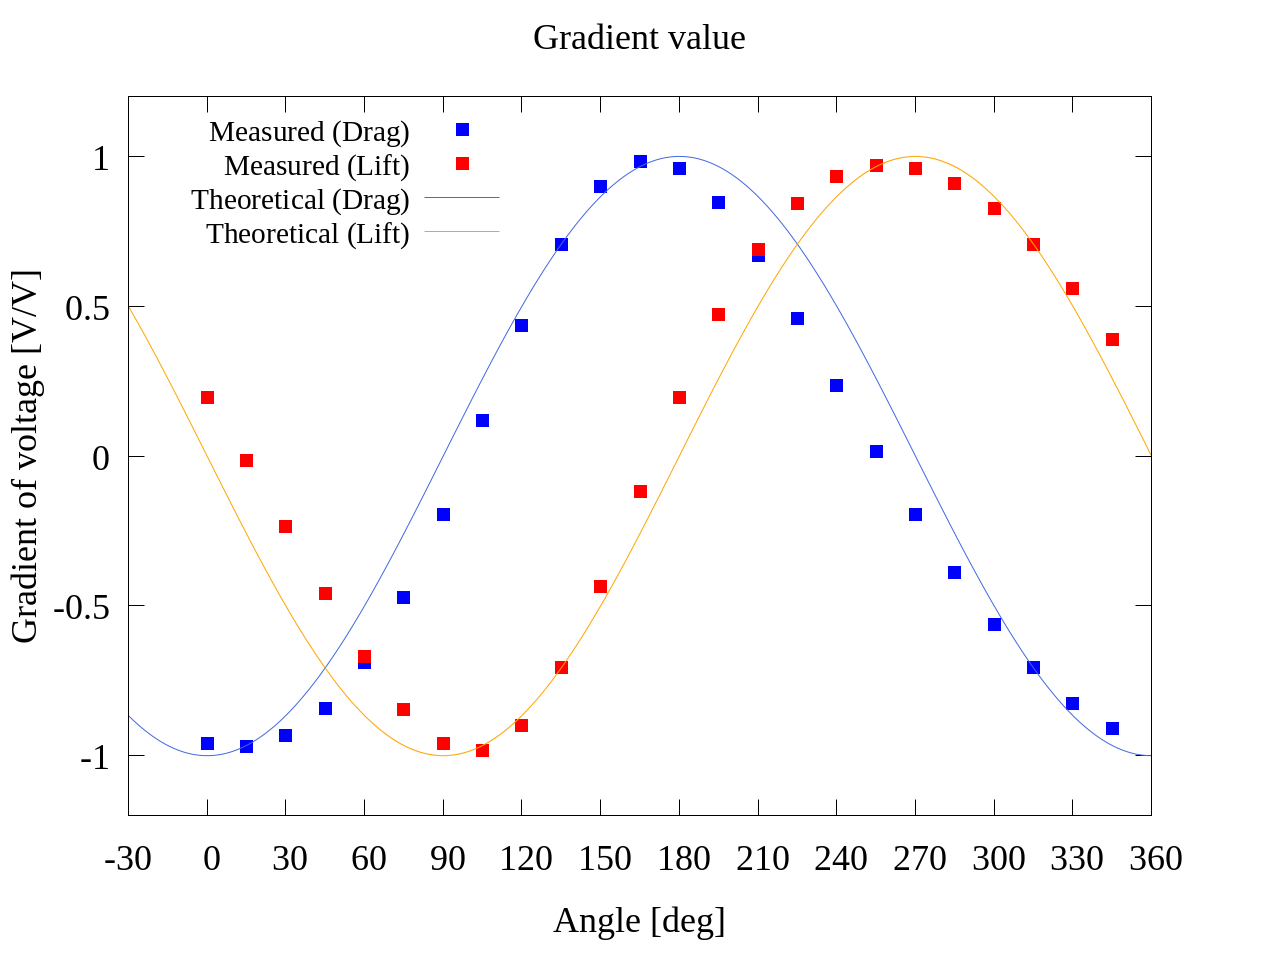
\includegraphics[width=65mm]{../../02_workspace/result/offset_dx=5.0_dy=-5.0/plot/20/20_adjust-value.png}
            \caption{Simulated data [Case 5]}
            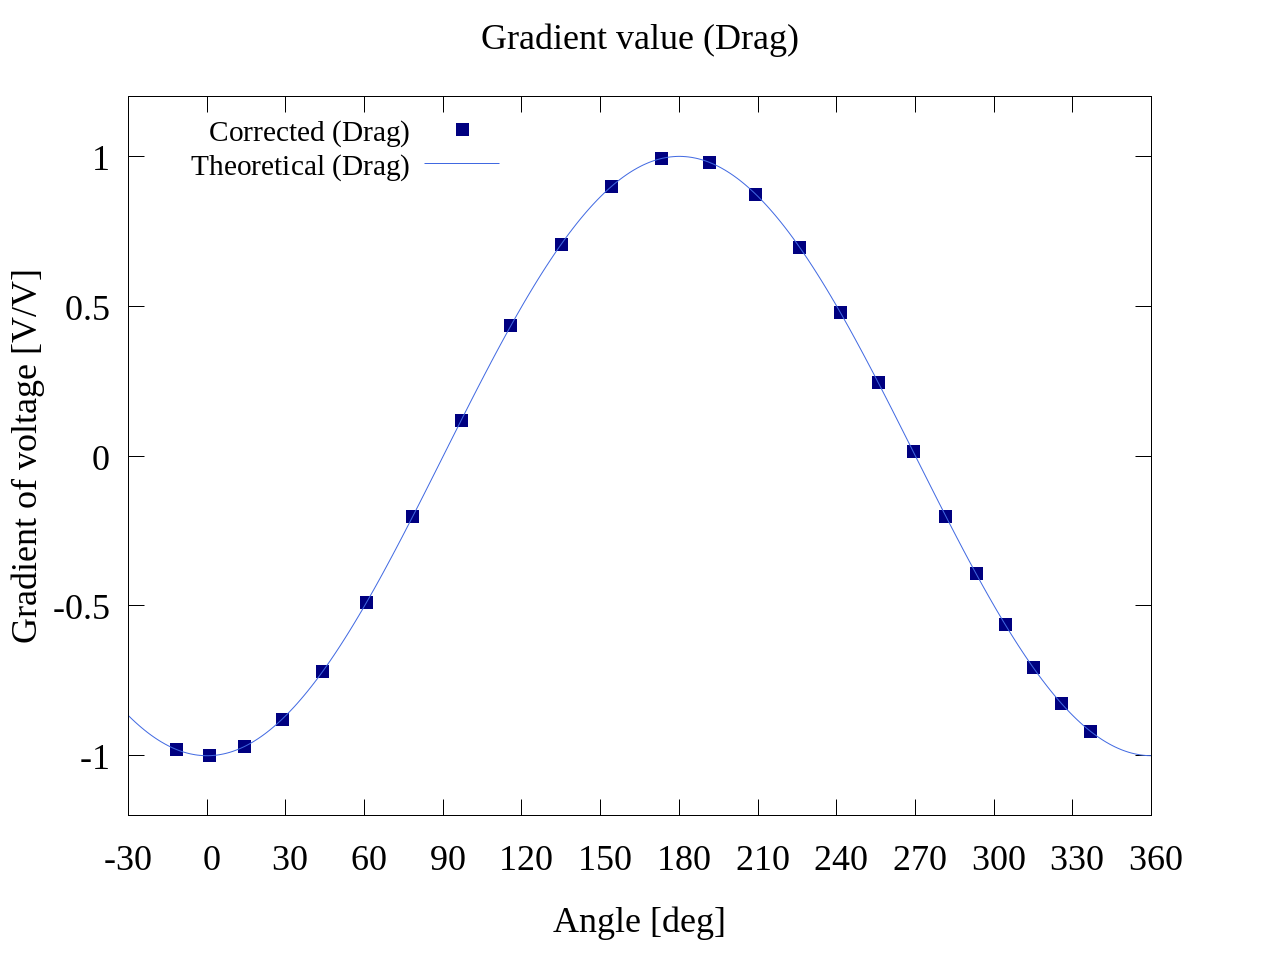
\includegraphics[width=65mm]{../../02_workspace/result/offset_dx=5.0_dy=-5.0/plot/21/21-2_corrected_offset_drag.png}
            \caption{Corrected data (Drag) [Case 5]}
            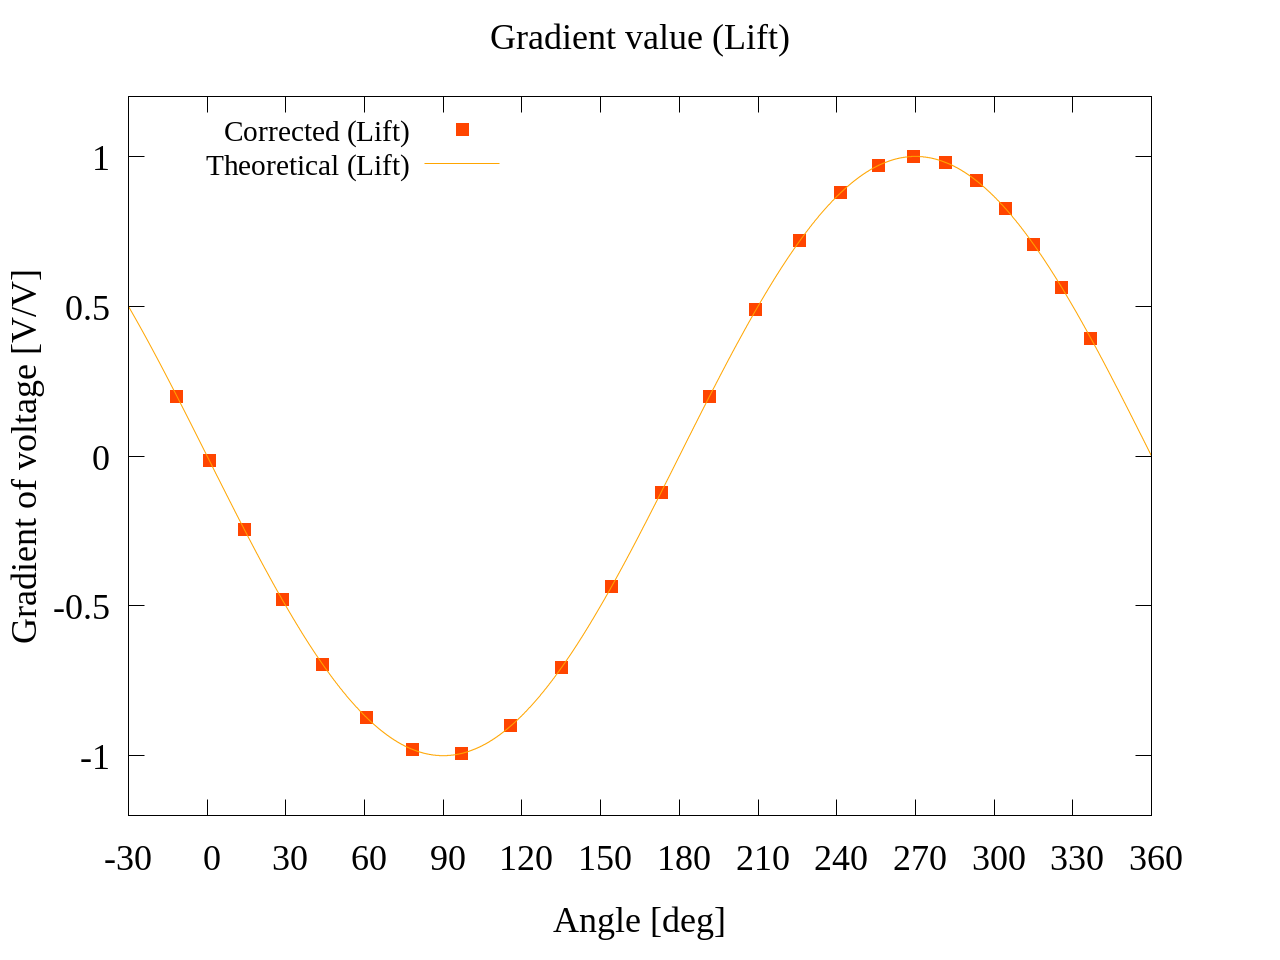
\includegraphics[width=65mm]{../../02_workspace/result/offset_dx=5.0_dy=-5.0/plot/21/21-2_corrected_offset_lift.png}
            \caption{Corrected data (Lift) [Case 5]}
        \end{center}
    \end{figure_here}

    \begin{figure_here}
        \subsubsection{テストデータ : Case 6}
        \vskip \baselineskip
        $\Delta x_\mathrm{test} = 10.0$ [mm],$\Delta x_\mathrm{test} = -5.0$ [mm]
        \footnotesize
        \begin{center}
            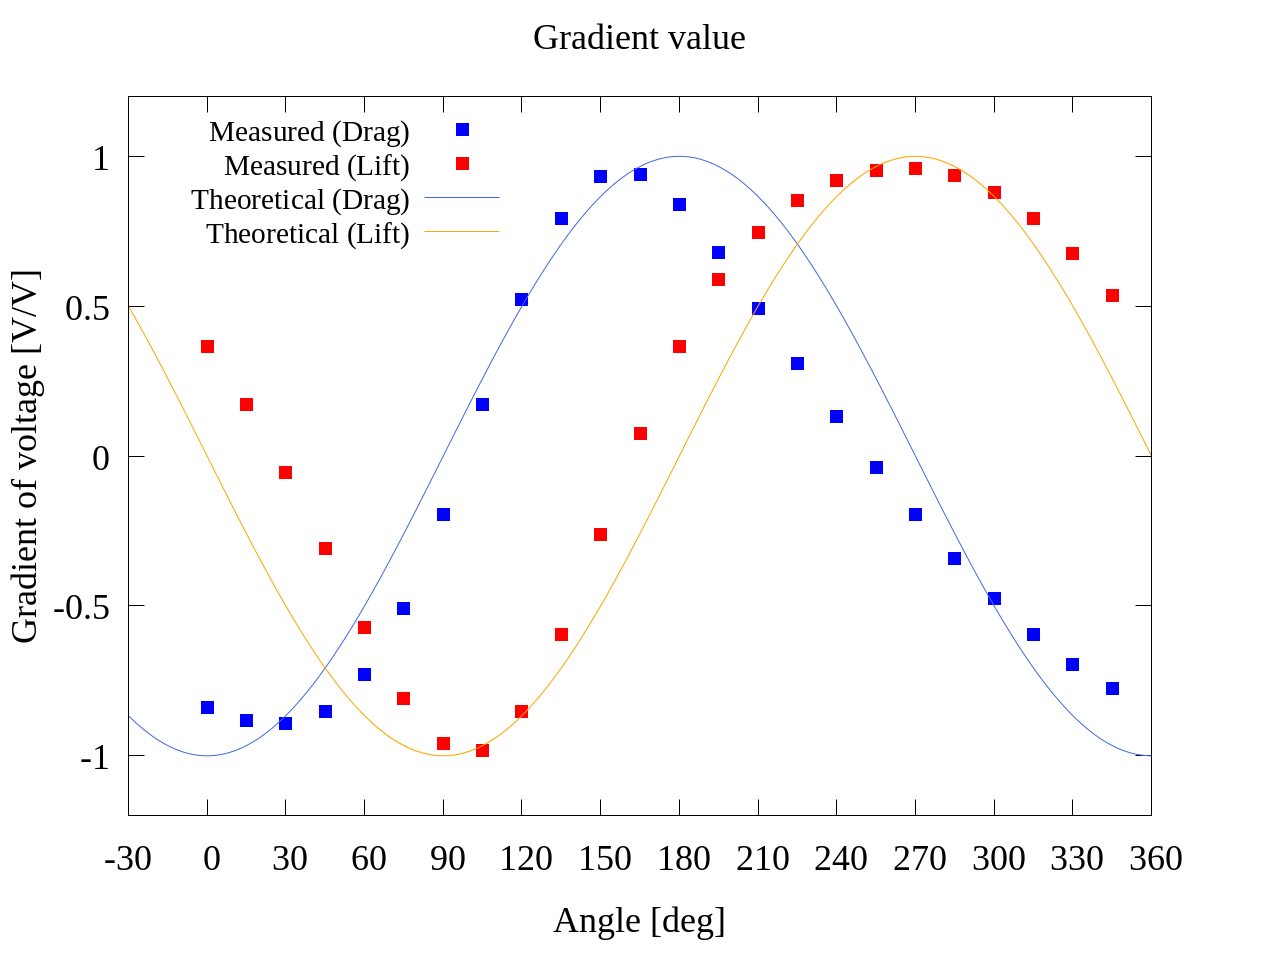
\includegraphics[width=65mm]{../../02_workspace/result/offset_dx=10.0_dy=-5.0/plot/20/20_adjust-value.png}
            \caption{Simulated data [Case 6]}
            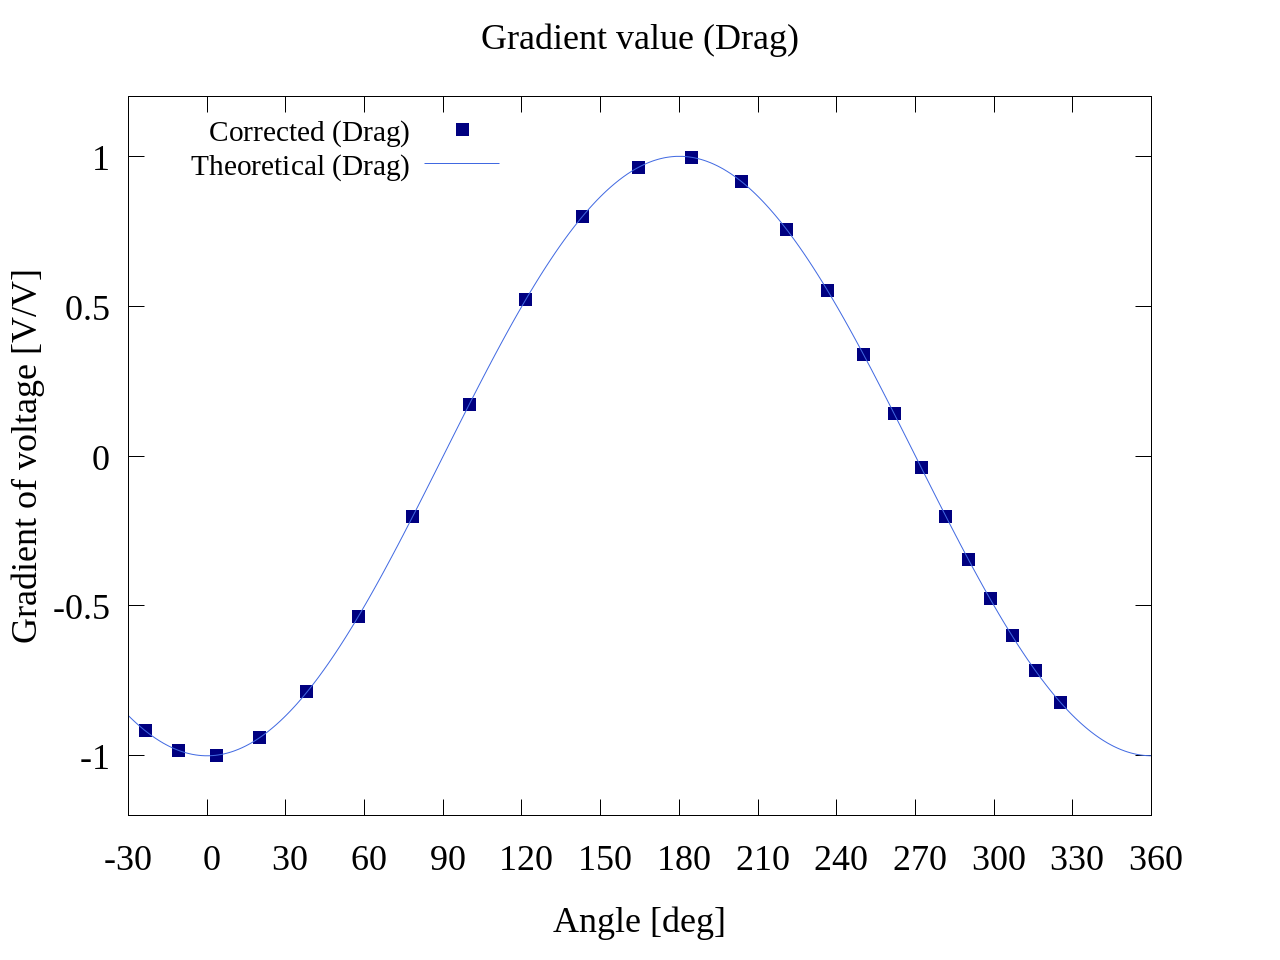
\includegraphics[width=65mm]{../../02_workspace/result/offset_dx=10.0_dy=-5.0/plot/21/21-2_corrected_offset_drag.png}
            \caption{Corrected data (Drag) [Case 6]}
            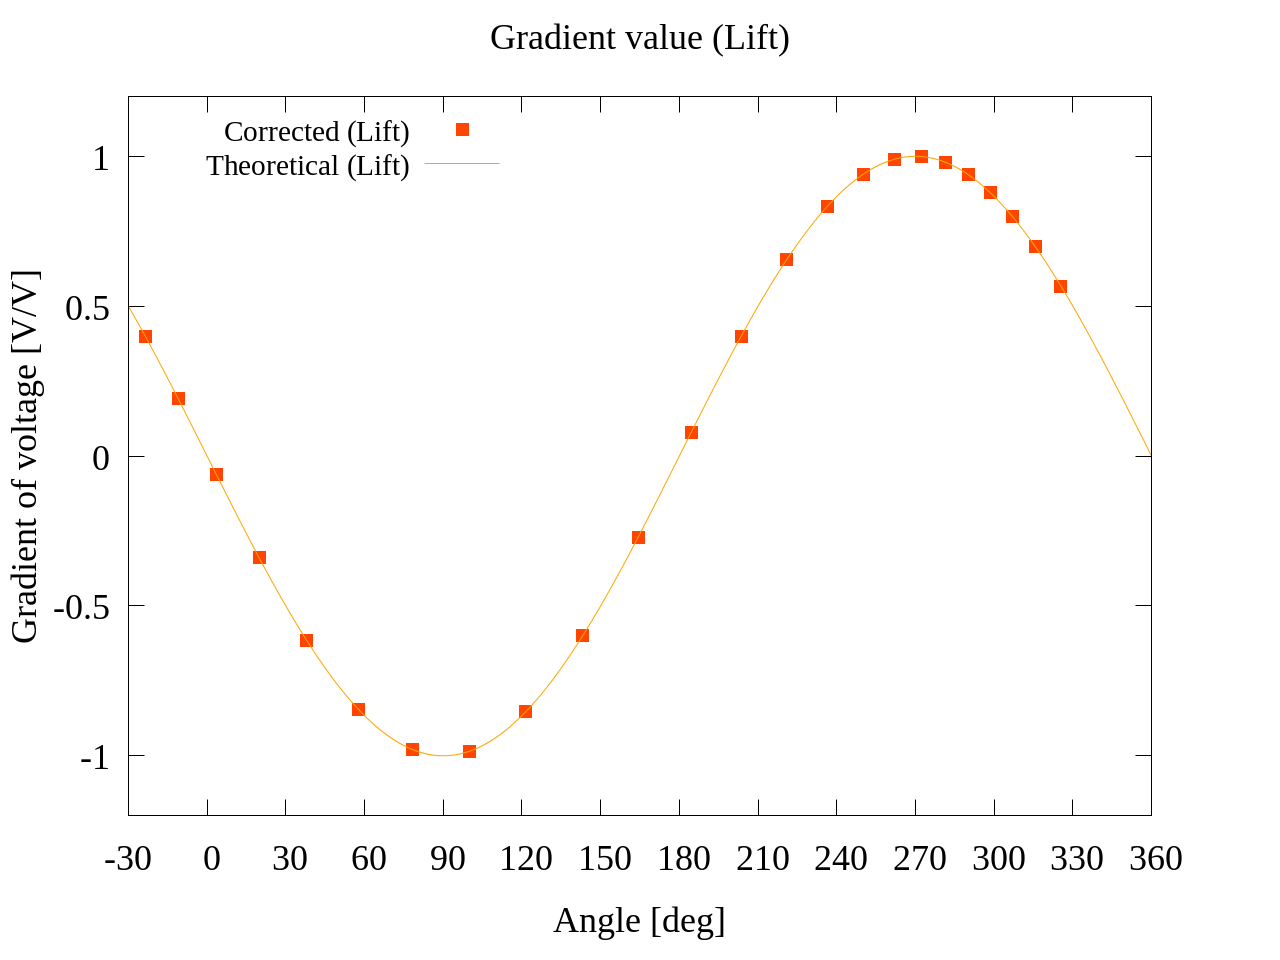
\includegraphics[width=65mm]{../../02_workspace/result/offset_dx=10.0_dy=-5.0/plot/21/21-2_corrected_offset_lift.png}
            \caption{Corrected data (Lift) [Case 6]}
        \end{center}
    \end{figure_here}
\end{multicols}

\subsection{複合状態における補正理論}

実際に校正実験を行う際には,座標系の回転,オフセットは同時に発生する.
したがって,上記の2つの補正理論を組み合わせて補正処理を行う必要がある.

\subsubsection{補正理論の適用順序}

作成した補正理論について,座標系の回転角$\theta_x$,$\theta_2$の特定の際に
離散フーリエ変換を適用することから,座標系のオフセットにおける補正理論を先に適用する必要がある.
また,上述のようにオフセットを考慮した場合,データ間隔が不等間隔となるため
回転角を特定するための離散フーリエ変換が適用できない.
したがって,ラグランジュ補間を用いて二次近似を行い,等間隔のデータを補完することとした.

\subsubsection{ラグランジュ補間}

一般にラグランジュ補間公式とは,$(x_1,f\left(x_1\right))$,$(x_2,f\left(x_2\right))$,
$(x_3,f \left(x_3\right))$,$\cdots$の点を通る関数$P\left(x\right)$を以下のように表す.

\begin{align}
    P\left(x\right)    & = \sum^{n+1}_{i=1} y_i \frac{f_i\left(x\right)}{f_i \left(x_i\right)} \\
    f_i \left(x\right) & = \prod_{k \neq i} \left(x - x_k\right)
\end{align}
\vskip \baselineskip

ここで,2次補間を行う場合,使用する3点を適切に選択する必要があるが
アルゴリズムを用いて処理を行いたい.
そこで,以下のような手順でラグランジュ補間を行った.

\subsubsection{使用するデータの選択}

校正実験では,15度ずつ測定しているため,計24点のデータを得ることができる.
座標系のオフセットにおける補正理論を用いた補正処理では,正規座標系における作用力とその角度が算出される.
しかし,離散フーリエ変換を適用するとき,等間隔のデータが必要となるため15度ごとの補間値を算出しなければならない.
ここで,必要な補間値の角度を$\theta$とするとき,
実際の作用力の角度$\varphi$との差
$\delta \theta$を絶対値で評価することで,その値$|\delta \theta|$が
最も小さくなる角度$\varphi$とその前後のデータを使用することで,$\theta$に最も近い3点を選択することができる.

\begin{align}
    \delta \theta = |\theta - \varphi|
\end{align}
\vskip \baselineskip

\subsubsection{テストデータへの適用 (3)}
上述の補正理論より座標系の回転・オフセットを考慮したテストデータを作成する.
任意の回転角$\theta_{1\;\mathrm{test}}$,$\theta_{2\; \mathrm{test}}$,
任意のオフセット$\Delta x_\mathrm{test}$,$\Delta y_\mathrm{test}$を与え,
複合状態における出力電圧勾配について,$x''$軸方向を$v_{x''\;\mathrm{test}}$,
$y''$軸方向を$v_{y''\;\mathrm{test}}$とするとき,以下のように表される.

\begin{align}
    \theta                  & = \frac{\pi}{180} \; i \;\left(i = 0, 1, 2, 3, \cdots\right)                                                       \\
    \alpha                  & = \sin^{-1} \left( \frac{\Delta x_\mathrm{test} \sin \theta - \Delta y_\mathrm{test} \cos \theta}{r} \right)       \\
    \varphi                 & = \theta - \sin^{-1}\left(\frac{\Delta x_\mathrm{test} \sin \theta - \Delta y_\mathrm{test} \cos \theta}{r}\right) \\
    \notag                                                                                                                                       \\
    v_{x'' \;\mathrm{test}} & = - \cos \alpha \cos \left(\varphi - \theta_{1\; \mathrm{test}} \right)                                            \\
    v_{y'' \;\mathrm{test}} & = - \cos \alpha \sin \left(\varphi - \theta_{2\; \mathrm{test}}\right)
\end{align}

また,今回を以下のTable のようなパラメータを用いた.

\begin{table}[htbp]
    \begin{center}
        \caption{Test data conditions (3)}
        \begin{tabular}{|p{30mm}|p{20mm}|p{20mm}|p{20mm}|p{20mm}|}
            \hline
            \multicolumn{1}{|c|}{}       & \multicolumn{1}{|c|}{$\theta_{1\;\mathrm{test}}$ [deg]} & \multicolumn{1}{|c|}{$\theta_{2\;\mathrm{test}}$ [deg]} & \multicolumn{1}{|c|}{$\Delta x_\mathrm{test}$ [mm]} & \multicolumn{1}{|c|}{$\Delta y_\mathrm{test}$ [mm]} \\ \hline
            \multicolumn{1}{|c|}{Case 7} & \multicolumn{1}{|c|}{10.0}                              & \multicolumn{1}{|c|}{-5.0}                              & \multicolumn{1}{|c|}{5.00}                          & \multicolumn{1}{|c|}{-2.50}                         \\ \hline
        \end{tabular}
    \end{center}
\end{table}

Case 7 に対する座標系の回転おける補正理論の適用過程について説明する.
はじめに,作成したテストデータを以下に示す.

\begin{figure}[htbp]
    \footnotesize
    \begin{center}
        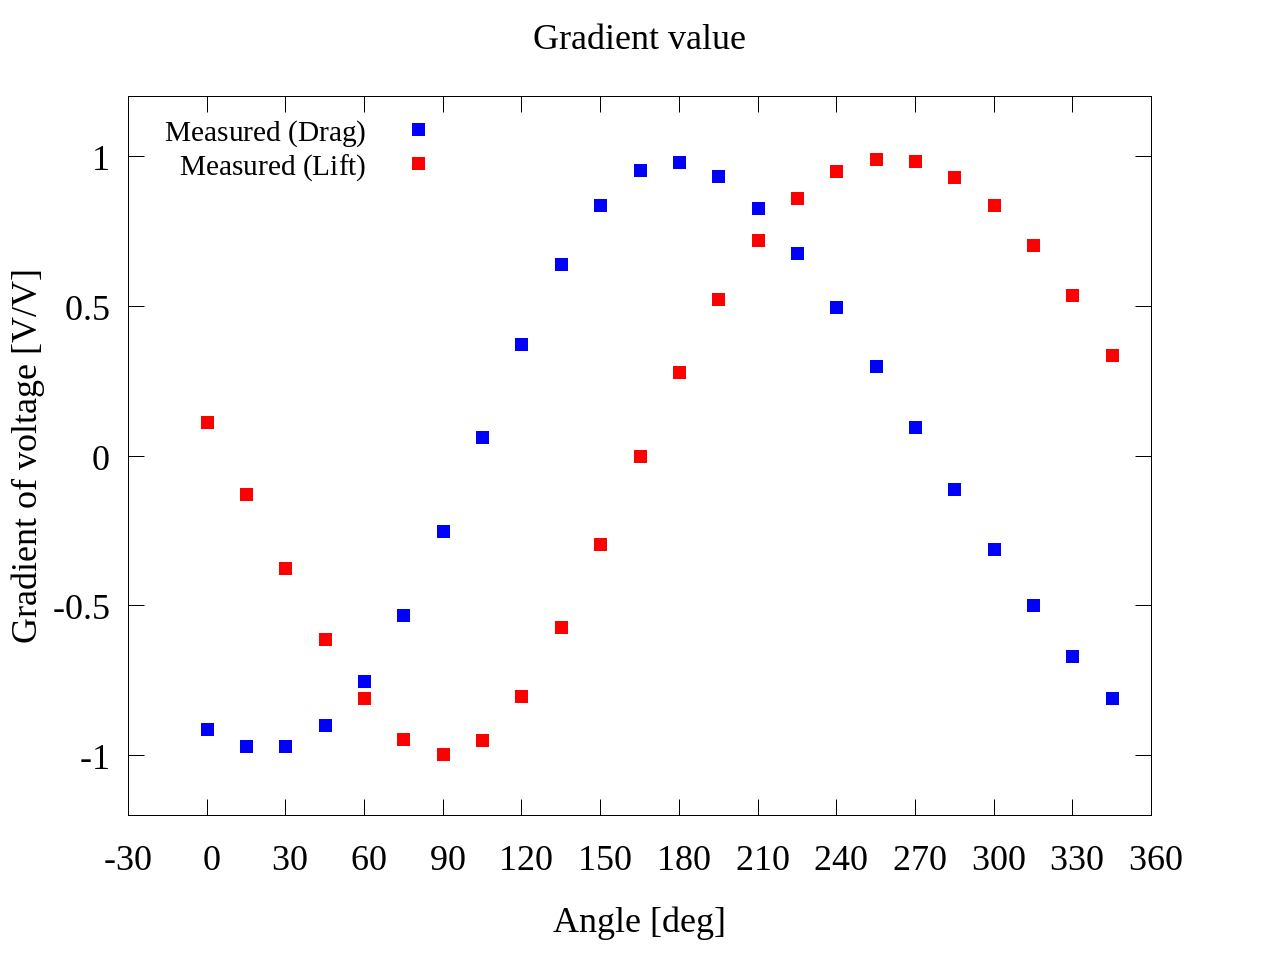
\includegraphics[width=95mm]{../../02_workspace/result/simulation_tx=10.0_ty=-5.0_dx=5.00_dy=-2.50/plot/05/05_summary-wave.png}
        \caption{Simulated data [Case 7]}
    \end{center}
\end{figure}

ここで,座標系のオフセットにおける補正理論を適用した結果を以下のFig.,Fig.に示す.

\begin{multicols}{2}
    \begin{figure_here}
        \begin{center}
            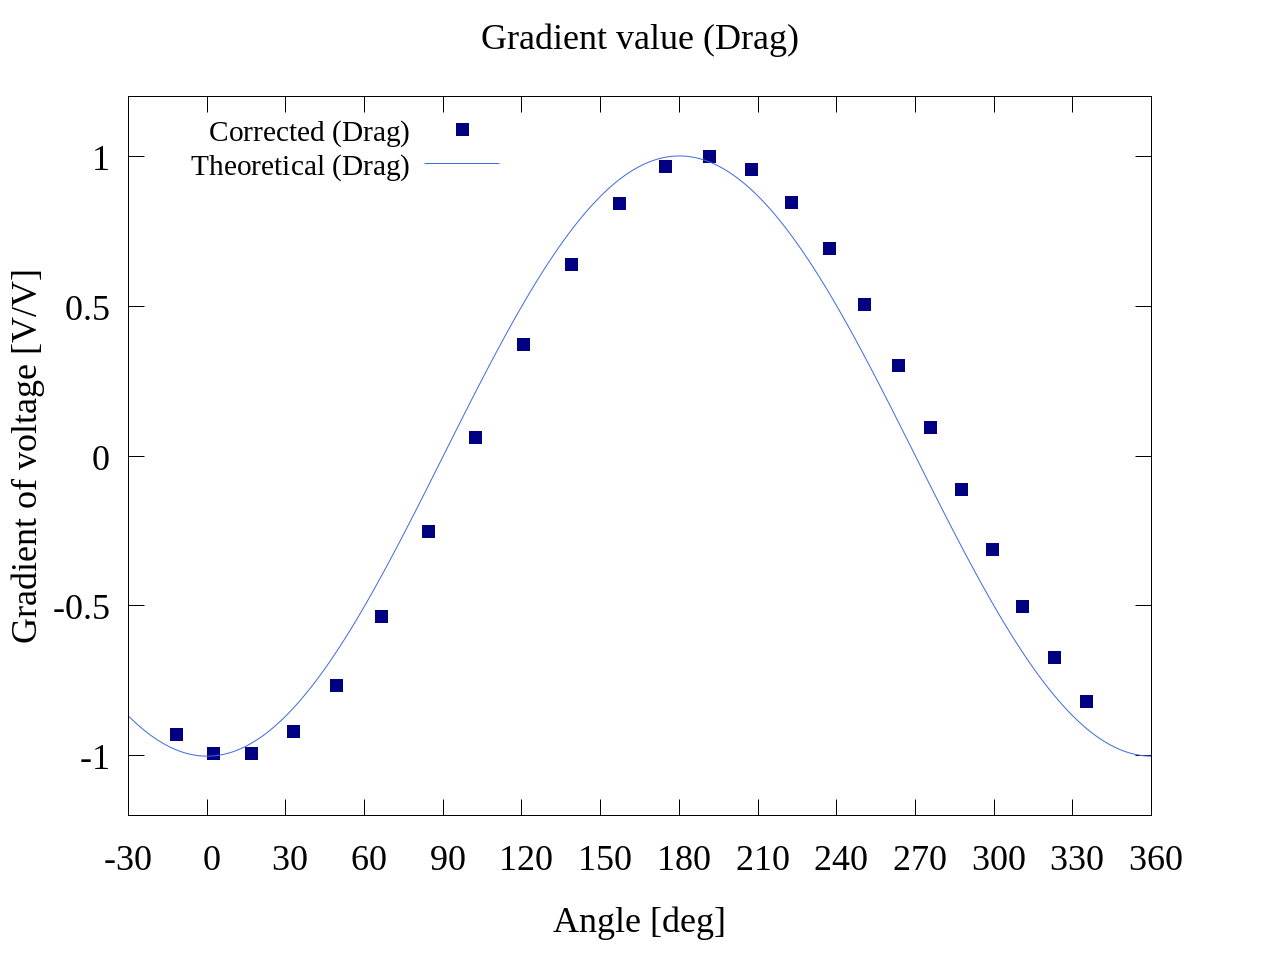
\includegraphics[width=65mm]{../../02_workspace/result/simulation_tx=10.0_ty=-5.0_dx=5.00_dy=-2.50/plot/21/21-2_corrected_offset_drag.png}
            \caption{Offset corrected value (Drag) [Case 7]}
            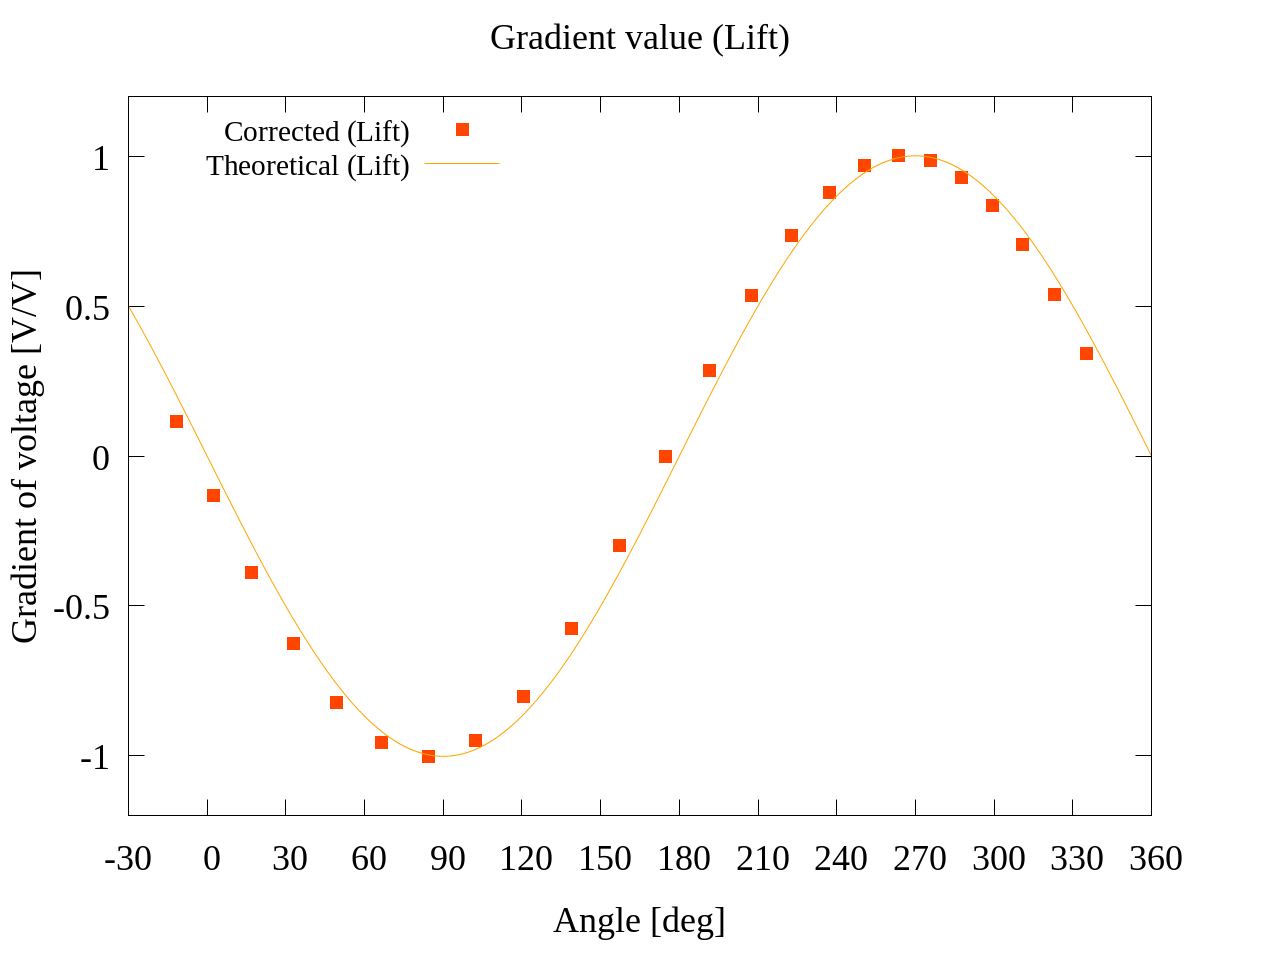
\includegraphics[width=65mm]{../../02_workspace/result/simulation_tx=10.0_ty=-5.0_dx=5.00_dy=-2.50/plot/21/21-2_corrected_offset_lift.png}
            \caption{Offset corrected value (lift) [Case 7]}
        \end{center}
    \end{figure_here}
\end{multicols}

理論曲線と比較して,波形の再現はされているが,位相差があるようにみえる.
また,プロットされたデータ間隔は異なることもわかる.
このとき,ラグランジュ補間を用いて,等間隔のデータを得るための処理を行う.
なお,データの採用点については上述の処理によって行うこととする.
ラグランジュ補間を行った結果を以下のFig.,Fig.に示す.

\begin{multicols}{2}
    \begin{figure_here}
        \begin{center}
            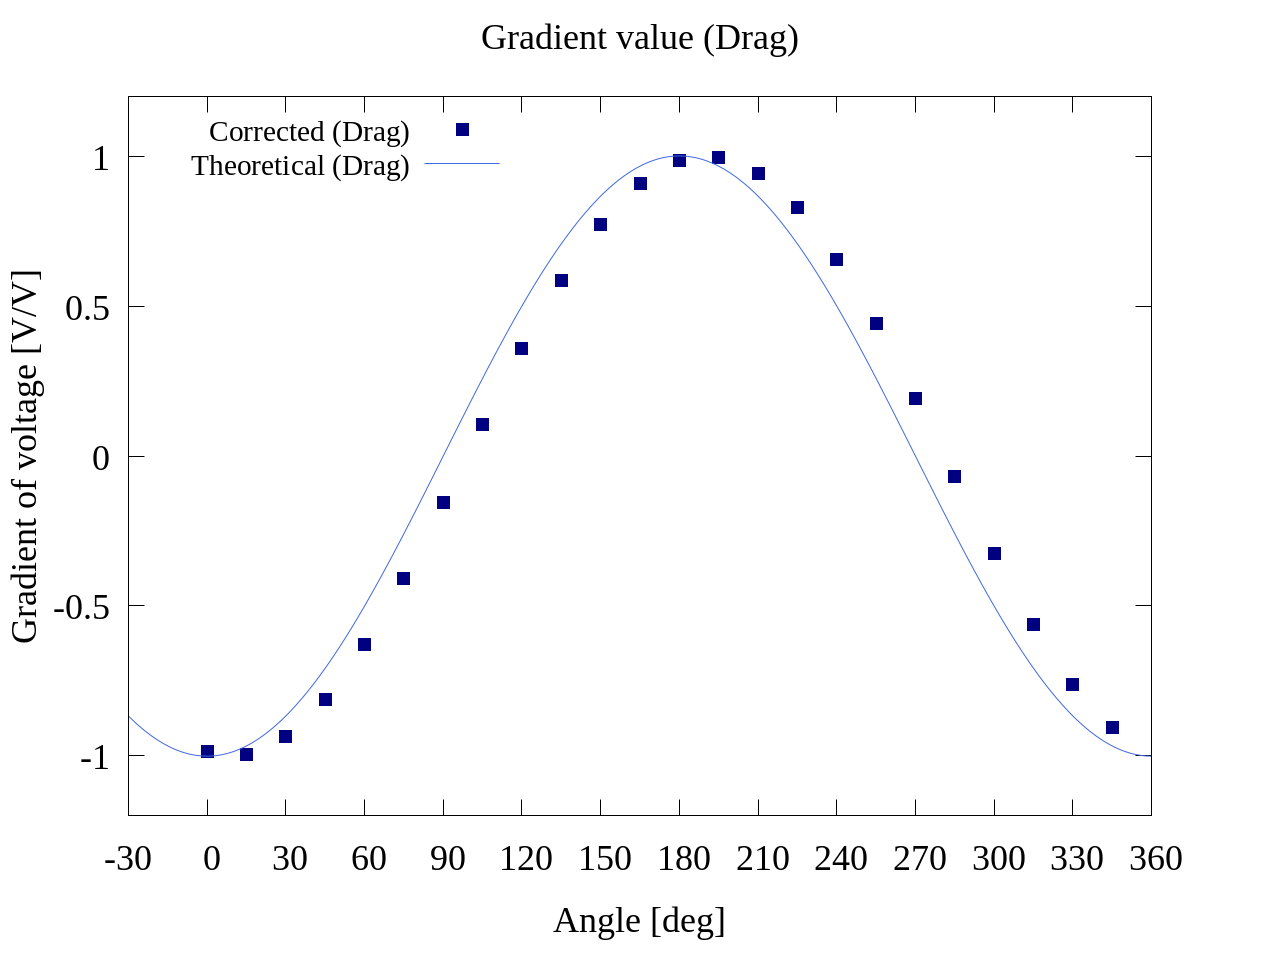
\includegraphics[width=65mm]{../../02_workspace/result/simulation_tx=10.0_ty=-5.0_dx=5.00_dy=-2.50/plot/21/21-3_interpolated_drag.png}
            \caption{Offset corrected value (Drag) [Case 7]}
            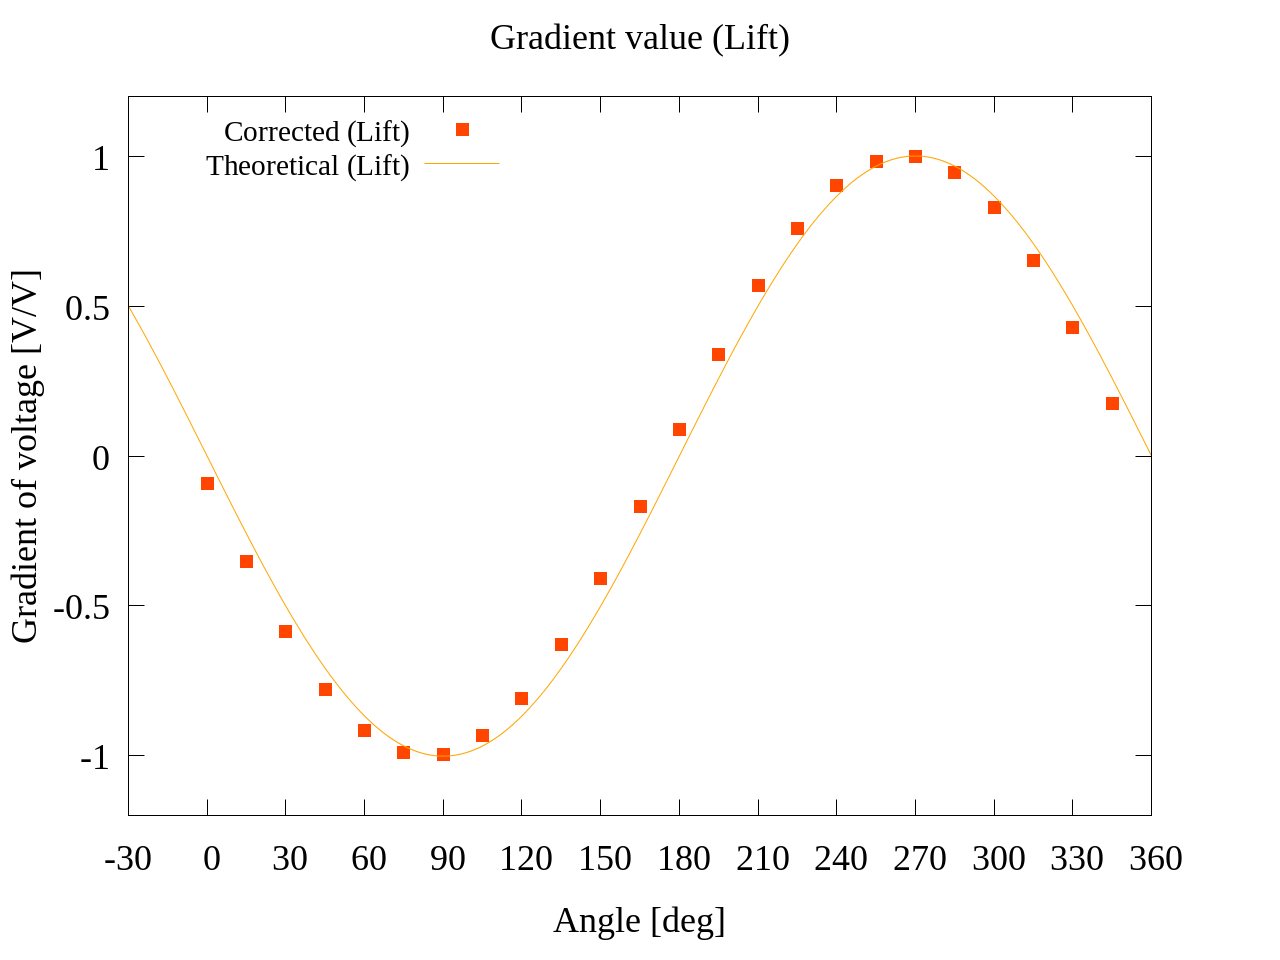
\includegraphics[width=65mm]{../../02_workspace/result/simulation_tx=10.0_ty=-5.0_dx=5.00_dy=-2.50/plot/21/21-3_interpolated_lift.png}
            \caption{Offset corrected value (lift) [Case 7]}
        \end{center}
    \end{figure_here}
\end{multicols}

上記のFig.,Fig.と比較すると等間隔のデータを得られていることがわかる.
次に,フーリエ変換を適用する.
このときの結果を以下のFig.,Fig.に示す.
また,波数1の成分についての算出値を以下のTable に示す.

\begin{table}[htbp]
    \begin{center}
        \caption{DFT result value [Case 7]}
        \begin{tabular}{|p{30mm}|p{20mm}|p{20mm}|}
            \hline
            \multicolumn{1}{|c|}{}     & \multicolumn{1}{|c|}{$Re$}    & \multicolumn{1}{|c|}{$Im$}   \\ \hline
            \multicolumn{1}{|c|}{Drag} & \multicolumn{1}{|c|}{-11.835} & \multicolumn{1}{|c|}{2.083}  \\ \hline
            \multicolumn{1}{|c|}{Lift} & \multicolumn{1}{|c|}{-1.081}  & \multicolumn{1}{|c|}{11.978} \\ \hline
        \end{tabular}
    \end{center}
\end{table}

\newpage

\begin{multicols}{2}
    \begin{figure_here}
        \begin{center}
            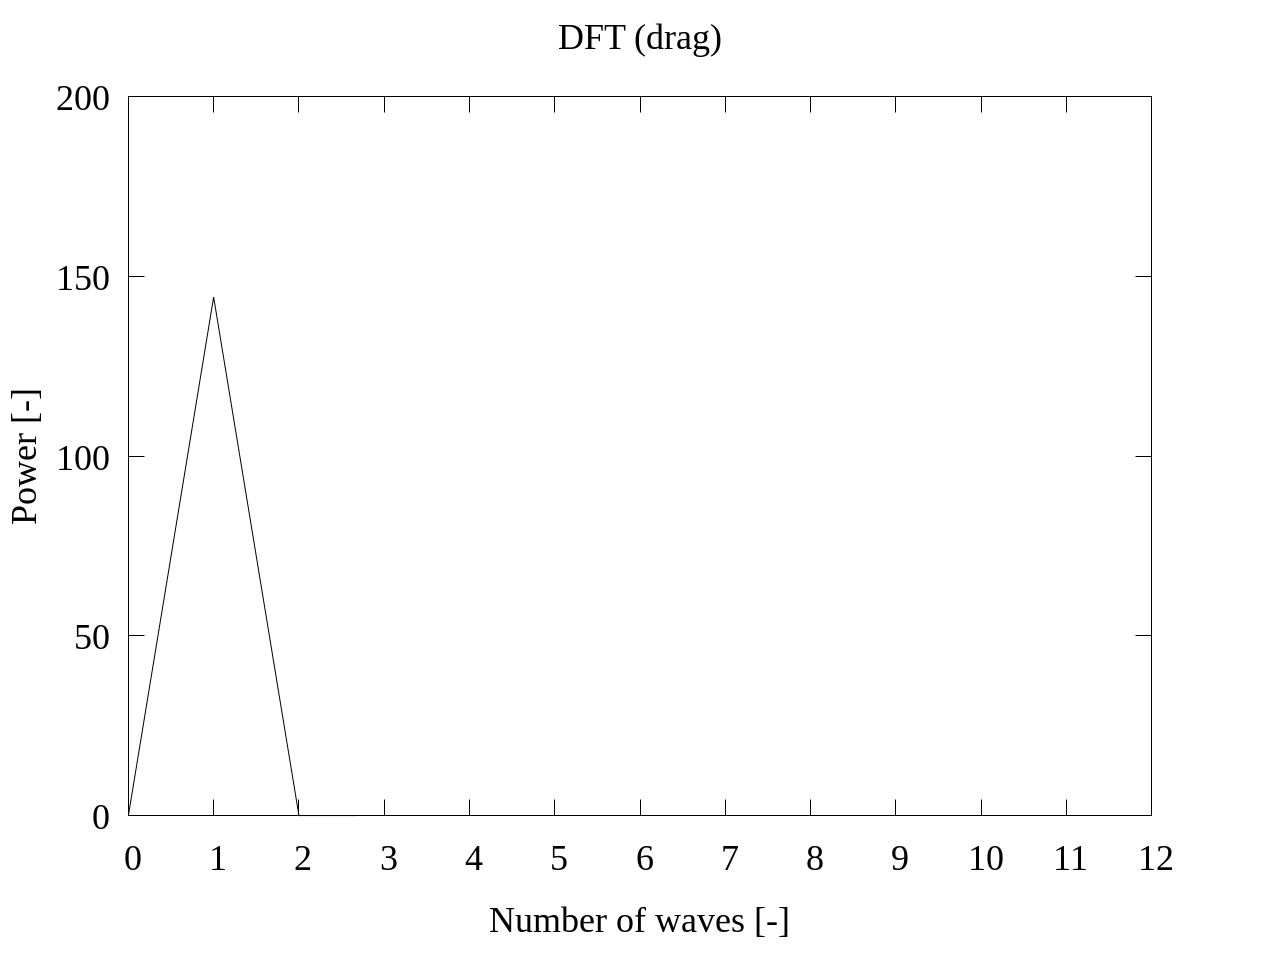
\includegraphics[width=65mm]{../../02_workspace/result/simulation_tx=10.0_ty=-5.0_dx=5.00_dy=-2.50/plot/07/07-3_dft-drag.png}
            \caption{DFT result (Drag) [Case 7]}
            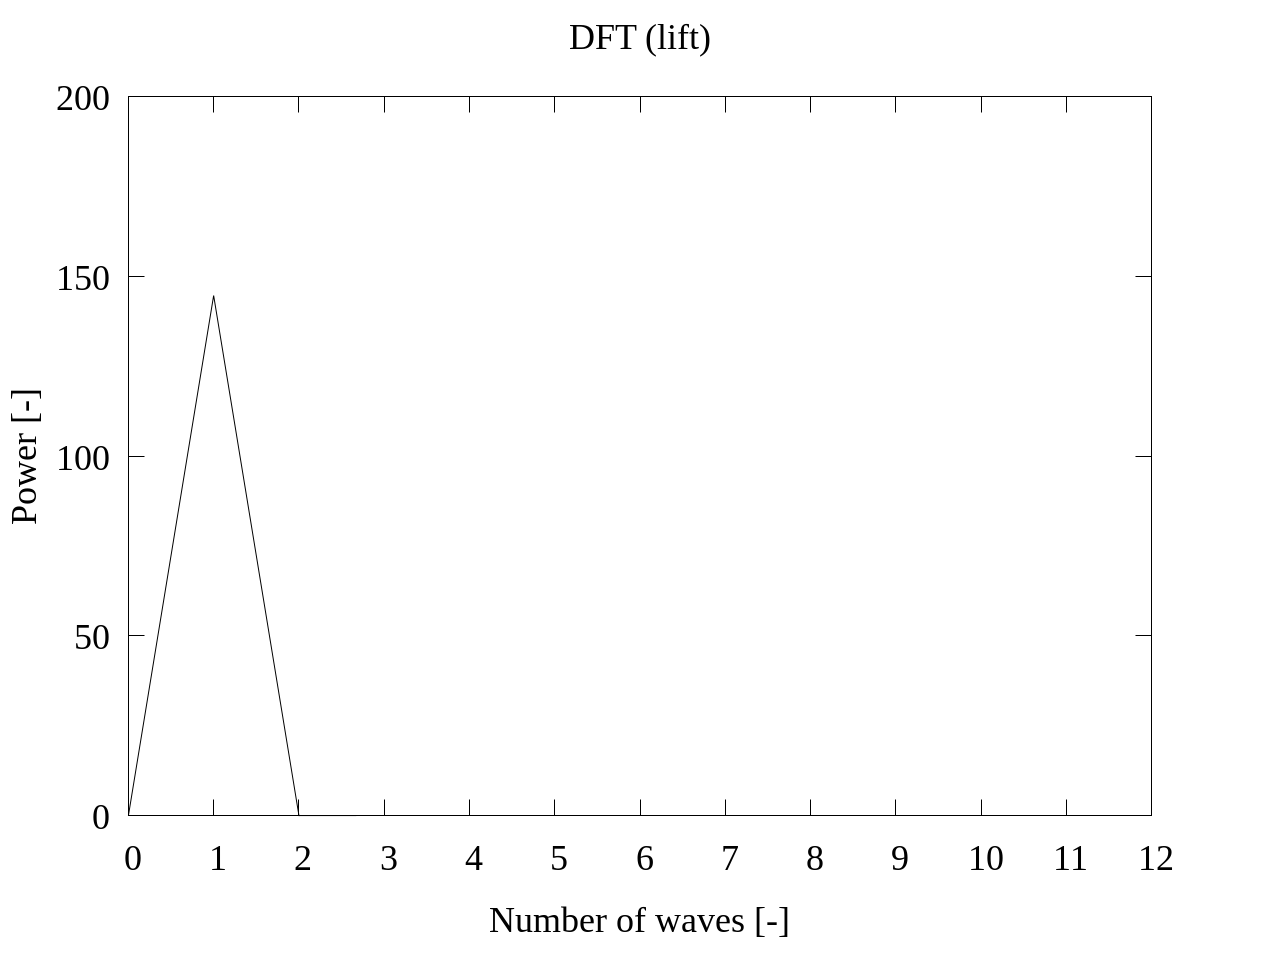
\includegraphics[width=65mm]{../../02_workspace/result/simulation_tx=10.0_ty=-5.0_dx=5.00_dy=-2.50/plot/07/07-4_dft-lift.png}
            \caption{DFT result (lift) [Case 7]}
        \end{center}
    \end{figure_here}
\end{multicols}

Fig. ,Fig. より,波数1についてピークがあることがわかり,
座標軸の回転における補正理論の適用結果と同様にデータの特徴を正しく捉えられているといえる.
ここで,Table について,式(),式(),式()より
回転角$\theta_x$,$\theta_y$をそれぞれ算出する.

\begin{table}[htbp]
    \begin{center}
        \caption{Specified rotation angle [Case 7]}
        \begin{tabular}{|p{30mm}|p{20mm}|p{20mm}|}
            \hline
            \multicolumn{1}{|c|}{}       & \multicolumn{1}{|c|}{$\theta_x$ [deg]} & \multicolumn{1}{|c|}{$\theta_y$ [deg]} \\ \hline
            \multicolumn{1}{|c|}{Case 7} & \multicolumn{1}{|c|}{10.018}           & \multicolumn{1}{|c|}{-5.158}           \\ \hline
        \end{tabular}
    \end{center}
\end{table}


結果より,算出された回転角$\theta_{1\;\mathrm{test}}$,$\theta_{2\;\mathrm{test}}$は
Table の Case 7 で設定したパラメータと比較すると,異なっていることがわかる.
これは,ラグランジュ補間公式を用いた2次近似による誤差が生じているためと考えられる.
ここで,誤差を算出すると,
\\
\vskip \baselineskip
\textgt{(誤差の算出と評価)}
\\
したがって,誤差は非常に小さいため無視できると考えられる.

また,算出した回転角$\theta_{1\;\mathrm{test}}$,$\theta_{2\;\mathrm{test}}$を用いて
座標系の回転における補正理論を適用した結果を以下のFig.,Fig.,に示す.

\begin{figure}
    \footnotesize
    \begin{center}
        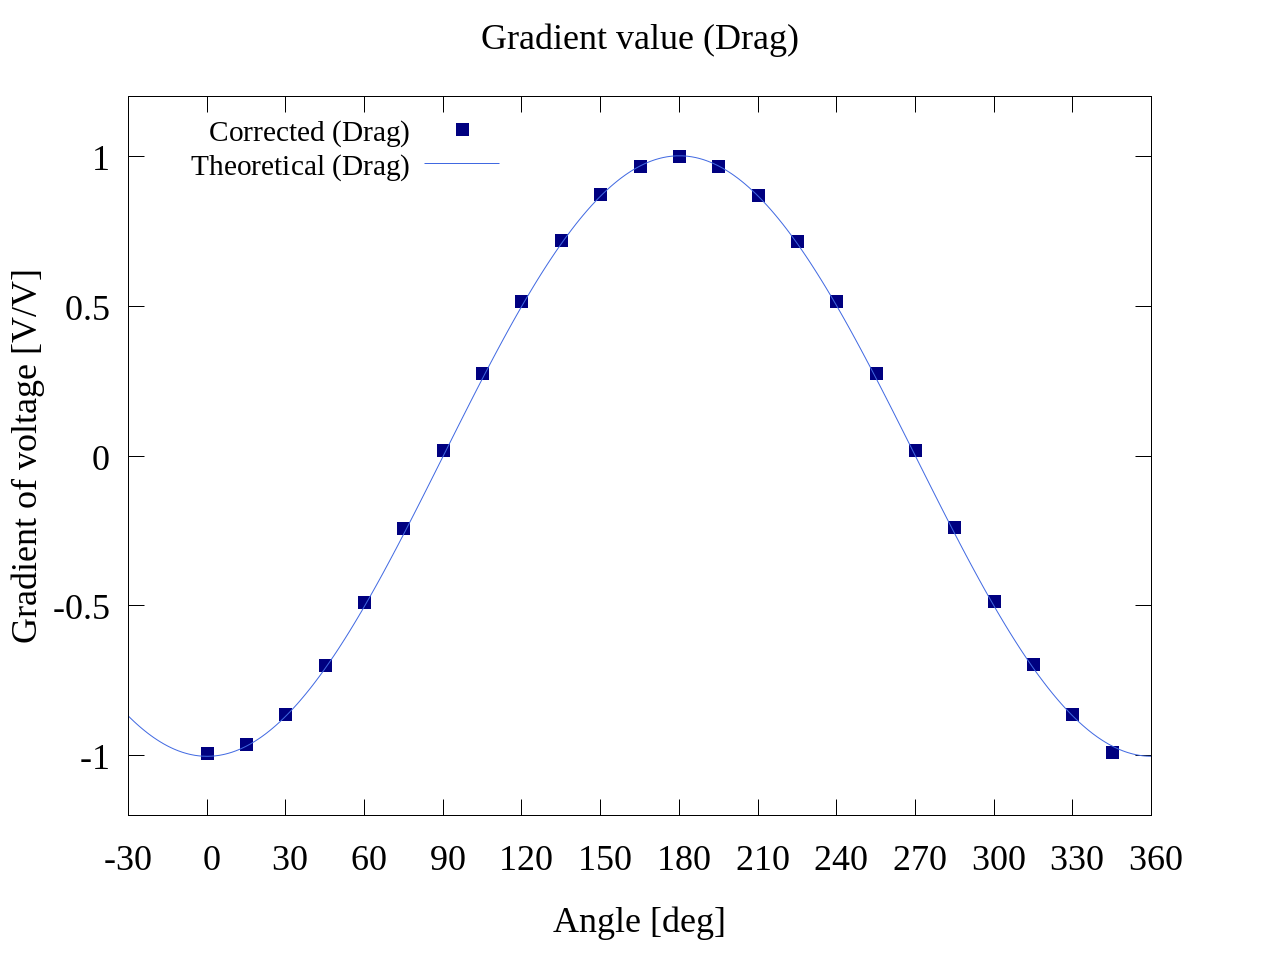
\includegraphics[width=95mm]{../../02_workspace/result/simulation_tx=10.0_ty=-5.0_dx=5.00_dy=-2.50/plot/21/21-4_corrected_angle_drag.png}
        \caption{Corrected data (Drag) [Case 7]}
        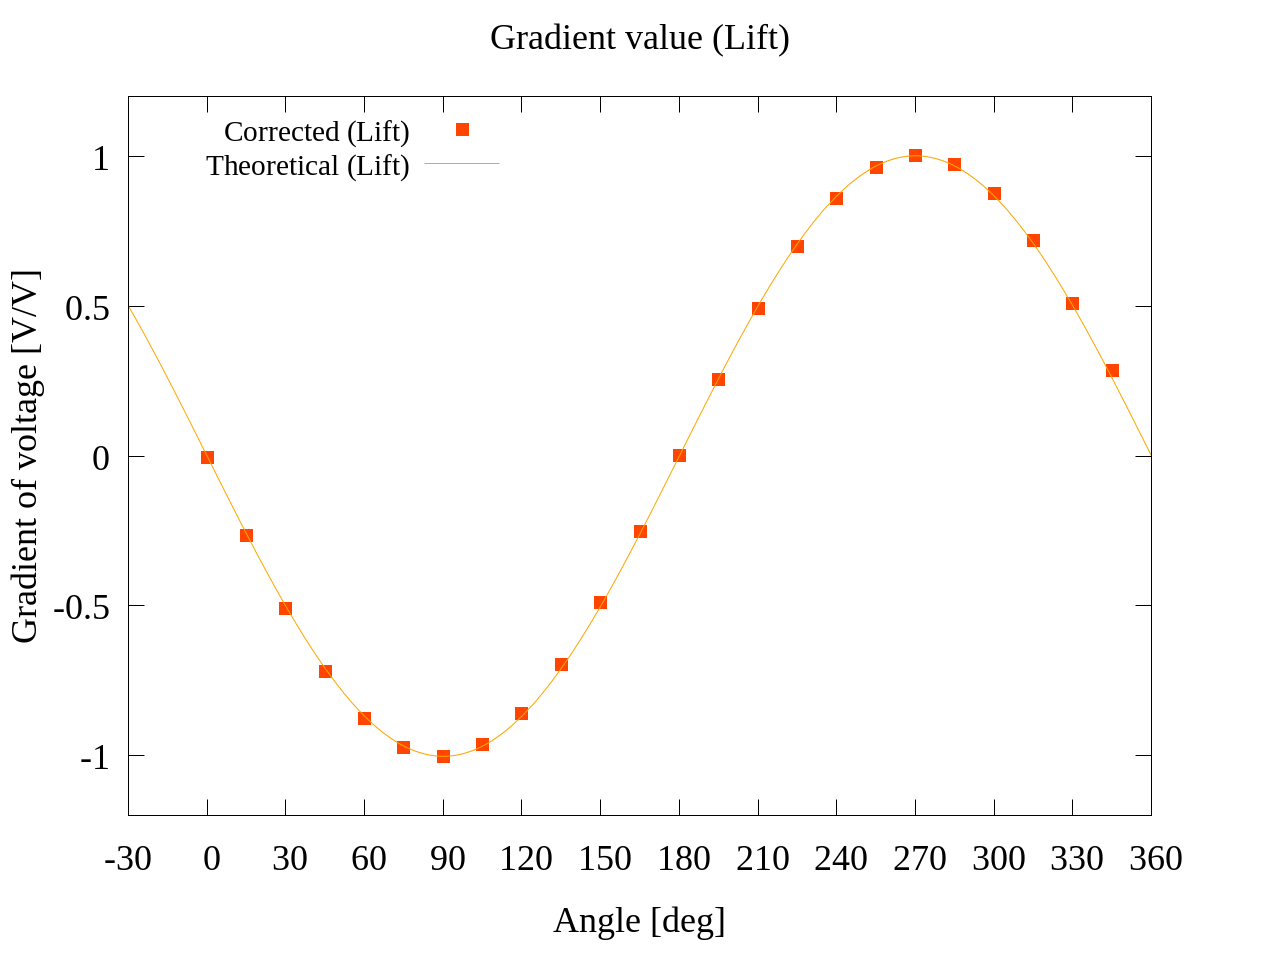
\includegraphics[width=95mm]{../../02_workspace/result/simulation_tx=10.0_ty=-5.0_dx=5.00_dy=-2.50/plot/21/21-4_corrected_angle_lift.png}
        \caption{Corrected data (Lift) [Case 7]}
    \end{center}
\end{figure}

% 同様に Case 8,Case 9 について,作成したテストデータとその補正結果および算出された回転角の値とその誤差について示す.

\newpage

\subsection{推定理論}
\newpage
\section{基礎実験(1)}

電圧と荷重の関係性の取得

\subsection{実験方法}

\subsection{実験結果}

\newpage
\section{基礎実験(2) (特性評価実験)}

\subsection{実験方法}

\subsection{実験結果}

\subsection{補正適用結果}

\subsection{テストデータの作成}

\newpage
\input{Section/6_applied_experiment.tex}

\newpage
\section*{謝辞}
\addcontentsline{toc}{section}{\gt 謝辞}
謝辞を述べる
\bibliography{ref_riron.bib}
\section*{付録}
\addcontentsline{toc}{subsection}{\gt 付録}
\end{document}
